\section{Analyse par regroupements d'actes}

\subsection{Actes sélectionnés} \label{section_2_1}



Dans cette partie nous allons analyser la chirurgie et médecine ambulatoire de manière générale, sur l'ensemble des actes sélectionnés dans la base de données CCAM. Dans les sous-parties suivantes, nous allons l'étudier par regroupements d'actes.\\

Soit $Y$ la variable d'intérêt (Part d'actes effectués en ambulatoire ou durée moyenne de séjour), $annee \in [\![2015,2019]\!]$ l'année et $etab \in [\![1,4]\!]$ la catégorie de l'établissement (On rappelle la correspondance : 1 pour les CHU, 2 pour les établissements publics, 3 pour les établissements privés lucratifs et 4 pour les établissements privés non-lucratifs). Ainsi, pour l'observation $i$, le modèle linéaire de base est:


\begin{multline}\label{eqn:equation_base}                                
  Y_i = \alpha + \sum_{j=2016}^{2019}[\beta_{A,j} . \mathbb{1+1}(annee_i=j)] +
\sum_{k=2}^{4}[\beta_{E,k} . \mathbb{1}(etab_i=k)] + \\
\sum_{j=2016}^{2019} \sum_{k=2}^{4}[\beta_{j,k}\mathbb{1}(annee_i=j).\mathbb{1}(etab_i=k)]
\end{multline} 

\bigskip

Ce modèle permet de retrouver les moyennes conditionnelles des tableaux \ref{part_ambu_tabu} et \ref{dms_tabu} via les coefficients $\alpha$, $\beta_{annee,j}$ et $\beta_{etab,k}$. L'utilisation de ce modèle linéaire permettra d'évaluer l'influence des variables, de constater s'il y existe une évolution temporelle significative et dans la suite, on pourra également ajouter des variables de contrôle. \textbf{Pour ce modèle, la référence (la constante) est la situation des CHU en 2015}.\\

Ici, le calcul des coefficients de la régression \ref{eqn:equation_base}, et des suivantes (\ref{eqn:cat} et \ref{eqn:annee}), est effectué avec une \textbf{pondération par le nombre d'actes ($nb\_actes$)}, les moyennes calculées correspondent donc à des moyennes pondérées par $nb\_actes$.  Les écarts-types des régressions sont calculés selon 3 différentes méthodes :
\begin{itemize}
    \item Calcul standard dans le cas d'homoscédasticité (\textit{default}).
    \item Calcul robuste lorsqu'on prend en compte l'hétéroscédasticité (\textit{robust}).
    \item Calcul robuste et avec des clusters, ici, on prend en compte le fait qu'on utilise des données de panel, pour gagner en robustesse, \textbf{on crée des clusters sur les couples ($FINESS\_ET$ , $acte$)}. En effet, l'observation d'un acte CCAM d'un établissement de l'année $i$ est corrélée à l'observation du même acte du même établissement de l'année $i'$  (\textit{robust and clustered}).
\end{itemize}

\newpage

Pour les moyennes conditionnées sur une seul variable (c'est-à-dire moyenne d'une catégorie sur l'ensemble des années ou d'une année sur l'ensemble des établissements), on effectue les régressions simples suivantes :

\begin{equation}\label{eqn:cat}
    Y_i = \alpha + \sum_{k=2}^{4}[\beta_{E,k} . \mathbb{1}(etab_i=k)]
\end{equation}

\begin{equation}\label{eqn:annee}
    Y_i = \alpha + \sum_{j=2016}^{2019}[\beta_{A,j} . \mathbb{1}(annee_i=j)]
\end{equation}


Ici, la référence correspond aux CHU pour la régression \ref{eqn:cat} et à l'année 2015 pour le modèle \ref{eqn:annee}.

\bigskip

\begin{table}[ht]
\centering
\caption{Pourcentage moyen d'actes effectués en ambulatoire (\%)} 
\label{part_ambu_tabu}
\begin{tabular}{r|cccc|c}
  \hline
 & CHU & Privé lucratif & Privé non lucratif & Public & Total \\ 
  \hline
2015 & 17.58 & 45.91 & 44.17 & 18.93 & 29.02 \\ 
  2016 & 18.43 & 46.88 & 44.34 & 19.80 & 29.62 \\ 
  2017 & 18.62 & 48.07 & 44.71 & 20.04 & 30.28 \\ 
  2018 & 18.96 & 49.78 & 45.38 & 20.64 & 31.22 \\ 
  2019 & 19.61 & 49.94 & 45.75 & 21.06 & 31.67 \\ 
  \hline
  Total & 18.64 & 48.12 & 44.88 & 20.09 & 30.36 \\ 
   \hline
\end{tabular}

\bigskip

\begin{tabular}{ccccc}
  \hline
Min. & 1er Qu. & Médiane & 3e Qu. & Max. \\ 
  \hline
0.00 & 0.00 & 8.60 & 68.12 & 100.00 \\ 
   \hline
\end{tabular}
\end{table}



\begin{table}[ht]
\centering
\caption{Durée moyenne des séjours en hôpitaux} 
\label{dms_tabu}
\begin{tabular}{r|cccc|c}
  \hline
 & CHU & Privé lucratif & Privé non lucratif & Public & Total \\ 
  \hline
2015 & 12.23 & 3.95 & 5.61 & 8.91 & 8.04 \\ 
  2016 & 11.47 & 3.88 & 5.61 & 8.69 & 7.80 \\ 
  2017 & 11.26 & 3.75 & 5.48 & 8.57 & 7.61 \\ 
  2018 & 11.18 & 3.59 & 5.33 & 8.42 & 7.47 \\ 
  2019 & 11.04 & 3.51 & 5.15 & 8.36 & 7.35 \\ 
  \hline
  Total & 11.44 & 3.74 & 5.43 & 8.59 & 7.65 \\ 
   \hline
\end{tabular}

\bigskip

\begin{tabular}{ccccc}
  \hline
Min. & 1er Qu. & Médiane & 3e Qu. & Max. \\ 
  \hline
0.00 & 1.22 & 6.51 & 10.61 & 670.50 \\ 
   \hline
\end{tabular}
\end{table}

\bigskip


Les deux tables ci-dessus présentent des moyennes obtenues grâce au modèle linéaire et sur l'ensemble des actes disponibles dans la table CCAM (même les actes non-sélectionnés). Le tableau \ref{part_ambu_tabu}, nous indique la part d'actes effectués en ambulatoire pour chaque année et chaque catégorie d'établissement. On constate déjà une tendance temporelle à la hausse, aussi bien en général (colonne "Total") que pour chaque catégorie. On s'aperçoit également que, de manière générale, les établissements publics ont bien moins recours à l'ambulatoire que les établissements privés, cela peut cependant être dû à la sélection des cas cliniques par ces derniers. On peut également noter que la tendance temporelle à la hausse est bien plus importante pour les cliniques privées à but lucratif, en effet, \textbf{l'augmentation de la part d'ambulatoire est au moins 2 fois plus importante} que pour les autres établissements.\\

Ces données sont en accord avec le tableau \ref{dms_tabu}, la durée moyenne de séjour a une tendance à la diminution, particulièrement marquée pour les CHU qui est aussi la catégorie d'établissement avec la durée moyenne la plus élevée, ce qui est cohérent compte-tenu du fait que ce sont les CHU qui traitent les cas les plus lourds.\\

Les tableaux \ref{reg_tous_actes} présentent les résultats des régressions \ref{eqn:cat}, \ref{eqn:annee} et \ref{eqn:equation_base}.\\


\begin{table}[!htbp] \centering 
  \caption{Modèles de base appliqué à la part d’actes en ambulatoire} 
  \label{reg_tous_actes} 
\begin{tabular}{@{\extracolsep{5pt}}lD{.}{.}{-3} D{.}{.}{-3} D{.}{.}{-3} } 
\\[-1.8ex]\hline 
\hline \\[-1.8ex] 
 & \multicolumn{3}{c}{\textit{Dependent variable:}} \\ 
\cline{2-4} 
\\[-1.8ex] & \multicolumn{3}{c}{Pourcentage d'ambulatoire} \\ 
 & \multicolumn{1}{c}{default} & \multicolumn{1}{c}{robust} & \multicolumn{1}{c}{robust and clustered} \\ 
\\[-1.8ex] & \multicolumn{1}{c}{(1)} & \multicolumn{1}{c}{(2)} & \multicolumn{1}{c}{(3)}\\ 
\hline \\[-1.8ex] 
 Privé lucratif & 29.481^{***} & 29.481^{***} & 29.481^{***} \\ 
  & (0.071) & (0.072) & (0.141) \\ 
  Privé non lucratif & 26.247^{***} & 26.247^{***} & 26.247^{***} \\ 
  & (0.107) & (0.112) & (0.218) \\ 
  Public & 1.453^{***} & 1.453^{***} & 1.453^{***} \\ 
  & (0.070) & (0.066) & (0.129) \\ 
  Constant & 18.638^{***} & 18.638^{***} & 18.638^{***} \\ 
  & (0.051) & (0.050) & (0.097) \\ 
 \hline \\[-1.8ex] 
Observations & \multicolumn{1}{c}{1,647,098} & \multicolumn{1}{c}{1,647,098} & \multicolumn{1}{c}{1,647,098} \\ 
R$^{2}$ & \multicolumn{1}{c}{0.132} & \multicolumn{1}{c}{0.132} & \multicolumn{1}{c}{0.132} \\ 
Adjusted R$^{2}$ & \multicolumn{1}{c}{0.132} & \multicolumn{1}{c}{0.132} & \multicolumn{1}{c}{0.132} \\ 
Residual Std. Error (df = 1647094) & \multicolumn{1}{c}{526.341} & \multicolumn{1}{c}{526.341} & \multicolumn{1}{c}{526.341} \\ 
F Statistic (df = 3; 1647094) & \multicolumn{1}{c}{83,403.180$^{***}$} & \multicolumn{1}{c}{83,403.180$^{***}$} & \multicolumn{1}{c}{83,403.180$^{***}$} \\ 
\hline 
\hline \\[-1.8ex]
\textit{Note:}  & \multicolumn{3}{r}{$^{*}$p$<$0.1; $^{**}$p$<$0.05; $^{***}$p$<$0.01} \\ 
\end{tabular}
\end{table}


\begin{table}[!htbp] \centering 
\begin{tabular}{@{\extracolsep{5pt}}lD{.}{.}{-3} D{.}{.}{-3} D{.}{.}{-3} } 
\\[-1.8ex]\hline 
\hline \\[-1.8ex] 
 & \multicolumn{3}{c}{\textit{Dependent variable:}} \\ 
\cline{2-4} 
\\[-1.8ex] & \multicolumn{3}{c}{Pourcentage d'ambulatoire} \\ 
 & \multicolumn{1}{c}{default} & \multicolumn{1}{c}{robust} & \multicolumn{1}{c}{robust and clustered} \\ 
\\[-1.8ex] & \multicolumn{1}{c}{(1)} & \multicolumn{1}{c}{(2)} & \multicolumn{1}{c}{(3)}\\ 
\hline \\[-1.8ex] 
 2016 & 0.601^{***} & 0.601^{***} & 0.601^{***} \\ 
  & (0.093) & (0.088) & (0.044) \\ 
  2017 & 1.266^{***} & 1.266^{***} & 1.266^{***} \\ 
  & (0.093) & (0.089) & (0.049) \\ 
  2018 & 2.203^{***} & 2.203^{***} & 2.203^{***} \\ 
  & (0.093) & (0.090) & (0.054) \\ 
  2019 & 2.649^{***} & 2.649^{***} & 2.649^{***} \\ 
  & (0.093) & (0.091) & (0.058) \\ 
  Constant & 29.017^{***} & 29.017^{***} & 29.017^{***} \\ 
  & (0.066) & (0.062) & (0.062) \\ 
 \hline \\[-1.8ex] 
Observations & \multicolumn{1}{c}{1,647,098} & \multicolumn{1}{c}{1,647,098} & \multicolumn{1}{c}{1,647,098} \\ 
R$^{2}$ & \multicolumn{1}{c}{0.001} & \multicolumn{1}{c}{0.001} & \multicolumn{1}{c}{0.001} \\ 
Adjusted R$^{2}$ & \multicolumn{1}{c}{0.001} & \multicolumn{1}{c}{0.001} & \multicolumn{1}{c}{0.001} \\ 
Residual Std. Error (df = 1647093) & \multicolumn{1}{c}{564.716} & \multicolumn{1}{c}{564.716} & \multicolumn{1}{c}{564.716} \\ 
F Statistic (df = 4; 1647093) & \multicolumn{1}{c}{278.160$^{***}$} & \multicolumn{1}{c}{278.160$^{***}$} & \multicolumn{1}{c}{278.160$^{***}$} \\ 
\hline 
\hline \\[-1.8ex] 
\textit{Note:}  & \multicolumn{3}{r}{$^{*}$p$<$0.1; $^{**}$p$<$0.05; $^{***}$p$<$0.01} \\ 
\end{tabular} 
\end{table}

\begin{table}[!htbp] \centering 
\scalebox{0.87}{\begin{tabular}{@{\extracolsep{5pt}}lD{.}{.}{-3} D{.}{.}{-3} D{.}{.}{-3} } 
\\[-1.8ex]\hline 
\hline \\[-1.8ex] 
 & \multicolumn{3}{c}{\textit{Dependent variable:}} \\ 
\cline{2-4} 
\\[-1.8ex] & \multicolumn{3}{c}{Pourcentage d'ambulatoire} \\ 
 & \multicolumn{1}{c}{default} & \multicolumn{1}{c}{robust} & \multicolumn{1}{c}{robust and clustered} \\ 
\\[-1.8ex] & \multicolumn{1}{c}{(1)} & \multicolumn{1}{c}{(2)} & \multicolumn{1}{c}{(3)}\\ 
\hline \\[-1.8ex] 
 Privé lucratif & 28.331^{***} & 28.331^{***} & 28.331^{***} \\ 
  & (0.159) & (0.154) & (0.154) \\ 
  Privé non lucratif & 26.587^{***} & 26.587^{***} & 26.587^{***} \\ 
  & (0.241) & (0.240) & (0.240) \\ 
  Public & 1.346^{***} & 1.346^{***} & 1.346^{***} \\ 
  & (0.157) & (0.140) & (0.140) \\ 
  2016 & 0.843^{***} & 0.843^{***} & 0.843^{***} \\ 
  & (0.162) & (0.150) & (0.072) \\ 
  2017 & 1.038^{***} & 1.038^{***} & 1.038^{***} \\ 
  & (0.162) & (0.152) & (0.084) \\ 
  2018 & 1.376^{***} & 1.376^{***} & 1.376^{***} \\ 
  & (0.162) & (0.155) & (0.092) \\ 
  2019 & 2.027^{***} & 2.027^{***} & 2.027^{***} \\ 
  & (0.163) & (0.158) & (0.101) \\ 
  Privé lucratif*2016 & 0.129 & 0.129 & 0.129 \\ 
  & (0.225) & (0.221) & (0.110) \\ 
  Privé non lucratif*2016 & -0.673^{**} & -0.673^{*} & -0.673^{***} \\ 
  & (0.342) & (0.346) & (0.175) \\ 
  Public*2016 & 0.027 & 0.027 & 0.027 \\ 
  & (0.222) & (0.201) & (0.098) \\ 
  Privé lucratif*2017 & 1.117^{***} & 1.117^{***} & 1.117^{***} \\ 
  & (0.225) & (0.223) & (0.125) \\ 
  Privé non lucratif*2017 & -0.496 & -0.496 & -0.496^{**} \\ 
  & (0.340) & (0.347) & (0.199) \\ 
  Public*2017 & 0.077 & 0.077 & 0.077 \\ 
  & (0.222) & (0.203) & (0.113) \\ 
  Privé lucratif*2018 & 2.496^{***} & 2.496^{***} & 2.496^{***} \\ 
  & (0.224) & (0.226) & (0.136) \\ 
  Privé non lucratif*2018 & -0.164 & -0.164 & -0.164 \\ 
  & (0.338) & (0.350) & (0.215) \\ 
  Public*2018 & 0.336 & 0.336 & 0.336^{***} \\ 
  & (0.222) & (0.207) & (0.124) \\ 
  Privé lucratif*2019 & 2.005^{***} & 2.005^{***} & 2.005^{***} \\ 
  & (0.225) & (0.227) & (0.146) \\ 
  Privé non lucratif*2019 & -0.441 & -0.441 & -0.441^{*} \\ 
  & (0.338) & (0.352) & (0.228) \\ 
  Public*2019 & 0.103 & 0.103 & 0.103 \\ 
  & (0.223) & (0.210) & (0.134) \\ 
  Constant & 17.582^{***} & 17.582^{***} & 17.582^{***} \\ 
  & (0.115) & (0.104) & (0.104) \\ 
 \hline \\[-1.8ex] 
Observations & \multicolumn{1}{c}{1,647,098} & \multicolumn{1}{c}{1,647,098} & \multicolumn{1}{c}{1,647,098} \\ 
R$^{2}$ & \multicolumn{1}{c}{0.133} & \multicolumn{1}{c}{0.133} & \multicolumn{1}{c}{0.133} \\ 
Adjusted R$^{2}$ & \multicolumn{1}{c}{0.133} & \multicolumn{1}{c}{0.133} & \multicolumn{1}{c}{0.133} \\ 
Residual Std. Error (df = 1647078) & \multicolumn{1}{c}{526.110} & \multicolumn{1}{c}{526.110} & \multicolumn{1}{c}{526.110} \\ 
F Statistic (df = 19; 1647078) & \multicolumn{1}{c}{13,257.670$^{***}$} & \multicolumn{1}{c}{13,257.670$^{***}$} & \multicolumn{1}{c}{13,257.670$^{***}$} \\ 
\hline 
\hline \\[-1.8ex]  
\end{tabular} 
}
\end{table} 

\newpage



Les tableaux \ref{part_ambu_select} et \ref{dms_select_moy} présentent les mêmes statistiques mais en se portant uniquement sur les actes sélectionnés. Les estimations des coefficients de la régression linéaire sont présentées dans la table \ref{reg_select}. On s'aperçoit que la sélection des actes pertinents nous permet de mieux capter les différences entre les établissements. C'est en accord avec la figure \ref{nuage_part_nb}. De plus, en se concentrant seulement sur les actes sélectionnés, le R\up{2} ajusté du modèle vaut 0.2001 contre 0.1326 pour l'ensemble des actes. \textbf{Dans la suite de cette partie, nous allons uniquement nous intéresser aux actes sélectionnés}.

\begin{table}[ht]
\centering
\caption{Pourcentage moyen d'actes sélectionnes effectués en ambulatoire (\%)} 
\label{part_ambu_select}
\begin{tabular}{r|cccc|c}
  \hline
 & CHU & Privé lucratif & Privé non lucratif & Public & Total \\ 
  \hline
2015 & 29.81 & 60.57 & 48.01 & 30.12 & 45.96 \\ 
  2016 & 31.31 & 62.30 & 49.25 & 31.97 & 47.29 \\ 
  2017 & 32.78 & 63.94 & 52.49 & 33.46 & 49.17 \\ 
  2018 & 34.33 & 65.43 & 54.42 & 35.17 & 50.91 \\ 
  2019 & 35.39 & 65.86 & 55.47 & 36.14 & 51.68 \\ 
  \hline
  Total & 32.76 & 63.66 & 52.11 & 33.41 & 49.05 \\ 
   \hline
\end{tabular}

\bigskip

\begin{tabular}{ccccc}
  \hline
Min. & 1er Qu. & Médiane & 3e Qu. & Max. \\ 
  \hline
0.00 & 18.48 & 48.88 & 80.66 & 100.00 \\ 
   \hline
\end{tabular}
\end{table}


\begin{table}[ht]
\centering
\caption{Durée moyenne des séjours en hôpitaux (actes sélectionnés)} 
\label{dms_select_moy}
\begin{tabular}{r|cccc|c}
  \hline
 & CHU & Privé lucratif & Privé non lucratif & Public & Total \\ 
  \hline
2015 & 8.23 & 1.86 & 3.64 & 6.36 & 4.43 \\ 
  2016 & 7.78 & 1.76 & 3.58 & 6.14 & 4.29 \\ 
  2017 & 7.61 & 1.67 & 3.32 & 5.91 & 4.11 \\ 
  2018 & 7.39 & 1.60 & 3.13 & 5.74 & 3.94 \\ 
  2019 & 7.26 & 1.58 & 3.04 & 5.68 & 3.88 \\ 
  \hline
  Total & 7.65 & 1.69 & 3.33 & 5.96 & 4.12 \\ 
   \hline
\end{tabular}

\bigskip

\begin{tabular}{ccccc}
  \hline
Min. & 1er Qu. & Médiane & 3e Qu. & Max. \\ 
  \hline
0.00 & 0.58 & 2.24 & 6.16 & 294.00 \\ 
   \hline
\end{tabular}
\end{table}


\bigskip

Grâce aux tableaux \ref{reg_select}, on observe que pour les régressions \ref{eqn:cat}, \ref{eqn:annee} et \ref{eqn:equation_base}, la variable \textit{Public} a une p-valeur assez élevée (supérieure à 0.1). Cela indique qu'a priori, le fait que l'établissement soit un CHU ou un établissement Public autre, n'a pas d'impact significatif sur la part d'actes effectués en ambulatoire.

Grâce au tableau \ref{dms_select_moy}, on constate également une forte différence entre le public et le privé, cependant, au vu des durées moyennes de séjours, cela peut être dû à une sélection des cas moins sévères par les établissements privés. Dans ce cas, les hôpitaux publics traitent les cas les plus complexes nécessitant plusieurs jours d'hospitalisation.\\


\begin{table}[!htbp] \centering 
  \caption{Modèles de base appliqué à la part d’actes sélectionnés en ambulatoire} 
  \label{reg_select} 
\begin{tabular}{@{\extracolsep{5pt}}lD{.}{.}{-3} D{.}{.}{-3} D{.}{.}{-3} } 
\\[-1.8ex]\hline 
\hline \\[-1.8ex] 
 & \multicolumn{3}{c}{\textit{Dependent variable:}} \\ 
\cline{2-4} 
\\[-1.8ex] & \multicolumn{3}{c}{Pourcentage d'ambulatoire} \\ 
 & \multicolumn{1}{c}{default} & \multicolumn{1}{c}{robust} & \multicolumn{1}{c}{robust and clustered} \\ 
\\[-1.8ex] & \multicolumn{1}{c}{(1)} & \multicolumn{1}{c}{(2)} & \multicolumn{1}{c}{(3)}\\ 
\hline \\[-1.8ex] 
 Privé lucratif & 30.901^{***} & 30.901^{***} & 30.901^{***} \\ 
  & (0.092) & (0.115) & (0.216) \\ 
  Privé non lucratif & 19.343^{***} & 19.343^{***} & 19.343^{***} \\ 
  & (0.142) & (0.180) & (0.336) \\ 
  Public & 0.645^{***} & 0.645^{***} & 0.645^{***} \\ 
  & (0.109) & (0.118) & (0.220) \\ 
  Constant & 32.763^{***} & 32.763^{***} & 32.763^{***} \\ 
  & (0.075) & (0.089) & (0.169) \\ 
 \hline \\[-1.8ex] 
Observations & \multicolumn{1}{c}{669,249} & \multicolumn{1}{c}{669,249} & \multicolumn{1}{c}{669,249} \\ 
R$^{2}$ & \multicolumn{1}{c}{0.196} & \multicolumn{1}{c}{0.196} & \multicolumn{1}{c}{0.196} \\ 
Adjusted R$^{2}$ & \multicolumn{1}{c}{0.196} & \multicolumn{1}{c}{0.196} & \multicolumn{1}{c}{0.196} \\ 
Residual Std. Error (df = 669245) & \multicolumn{1}{c}{355.704} & \multicolumn{1}{c}{355.704} & \multicolumn{1}{c}{355.704} \\ 
F Statistic (df = 3; 669245) & \multicolumn{1}{c}{54,393.270$^{***}$} & \multicolumn{1}{c}{54,393.270$^{***}$} & \multicolumn{1}{c}{54,393.270$^{***}$} \\ 
\hline 
\hline \\[-1.8ex] 
\end{tabular} 

\bigskip

\begin{tabular}{@{\extracolsep{5pt}}lD{.}{.}{-3} D{.}{.}{-3} D{.}{.}{-3} } 
\\[-1.8ex]\hline 
\hline \\[-1.8ex] 
 & \multicolumn{3}{c}{\textit{Dependent variable:}} \\ 
\cline{2-4} 
\\[-1.8ex] & \multicolumn{3}{c}{Pourcentage d'ambulatoire} \\ 
 & \multicolumn{1}{c}{default} & \multicolumn{1}{c}{robust} & \multicolumn{1}{c}{robust and clustered} \\ 
\\[-1.8ex] & \multicolumn{1}{c}{(1)} & \multicolumn{1}{c}{(2)} & \multicolumn{1}{c}{(3)}\\ 
\hline \\[-1.8ex] 
 2016 & 1.330^{***} & 1.330^{***} & 1.330^{***} \\ 
  & (0.129) & (0.143) & (0.079) \\ 
  2017 & 3.207^{***} & 3.207^{***} & 3.207^{***} \\ 
  & (0.128) & (0.143) & (0.088) \\ 
  2018 & 4.948^{***} & 4.948^{***} & 4.948^{***} \\ 
  & (0.127) & (0.144) & (0.095) \\ 
  2019 & 5.714^{***} & 5.714^{***} & 5.714^{***} \\ 
  & (0.127) & (0.144) & (0.100) \\ 
  Constant & 45.962^{***} & 45.962^{***} & 45.962^{***} \\ 
  & (0.091) & (0.099) & (0.099) \\ 
 \hline \\[-1.8ex] 
Observations & \multicolumn{1}{c}{669,249} & \multicolumn{1}{c}{669,249} & \multicolumn{1}{c}{669,249} \\ 
R$^{2}$ & \multicolumn{1}{c}{0.004} & \multicolumn{1}{c}{0.004} & \multicolumn{1}{c}{0.004} \\ 
Adjusted R$^{2}$ & \multicolumn{1}{c}{0.004} & \multicolumn{1}{c}{0.004} & \multicolumn{1}{c}{0.004} \\ 
Residual Std. Error (df = 669244) & \multicolumn{1}{c}{395.870} & \multicolumn{1}{c}{395.870} & \multicolumn{1}{c}{395.870} \\ 
F Statistic (df = 4; 669244) & \multicolumn{1}{c}{707.637$^{***}$} & \multicolumn{1}{c}{707.637$^{***}$} & \multicolumn{1}{c}{707.637$^{***}$} \\ 
\hline 
\hline \\[-1.8ex] 
\textit{Note:}  & \multicolumn{3}{r}{$^{*}$p$<$0.1; $^{**}$p$<$0.05; $^{***}$p$<$0.01} \\ 
\end{tabular} 
\end{table} 


\begin{table}[!htbp] \centering  
\scalebox{0.87}{\begin{tabular}{@{\extracolsep{5pt}}lD{.}{.}{-3} D{.}{.}{-3} D{.}{.}{-3} } 
\\[-1.8ex]\hline 
\hline \\[-1.8ex] 
 & \multicolumn{3}{c}{\textit{Dependent variable:}} \\ 
\cline{2-4} 
\\[-1.8ex] & \multicolumn{3}{c}{Pourcentage d'ambulatoire} \\ 
 & \multicolumn{1}{c}{default} & \multicolumn{1}{c}{robust} & \multicolumn{1}{c}{robust and clustered} \\ 
\\[-1.8ex] & \multicolumn{1}{c}{(1)} & \multicolumn{1}{c}{(2)} & \multicolumn{1}{c}{(3)}\\ 
\hline \\[-1.8ex] 
 Privé lucratif & 30.760^{***} & 30.760^{***} & 30.760^{***} \\ 
  & (0.209) & (0.247) & (0.247) \\ 
  Privé non lucratif & 18.206^{***} & 18.206^{***} & 18.206^{***} \\ 
  & (0.327) & (0.392) & (0.392) \\ 
  Public & 0.313 & 0.313 & 0.313 \\ 
  & (0.246) & (0.248) & (0.248) \\ 
  2016 & 1.503^{***} & 1.503^{***} & 1.503^{***} \\ 
  & (0.240) & (0.270) & (0.142) \\ 
  2017 & 2.979^{***} & 2.979^{***} & 2.979^{***} \\ 
  & (0.239) & (0.274) & (0.164) \\ 
  2018 & 4.522^{***} & 4.522^{***} & 4.522^{***} \\ 
  & (0.239) & (0.279) & (0.180) \\ 
  2019 & 5.584^{***} & 5.584^{***} & 5.584^{***} \\ 
  & (0.239) & (0.282) & (0.193) \\ 
  Privé lucratif*2016 & 0.235 & 0.235 & 0.235 \\ 
  & (0.294) & (0.354) & (0.193) \\ 
  Privé non lucratif*2016 & -0.269 & -0.269 & -0.269 \\ 
  & (0.462) & (0.563) & (0.317) \\ 
  Public*2016 & 0.346 & 0.346 & 0.346^{*} \\ 
  & (0.347) & (0.356) & (0.196) \\ 
  Privé lucratif*2017 & 0.393 & 0.393 & 0.393^{*} \\ 
  & (0.292) & (0.357) & (0.218) \\ 
  Privé non lucratif*2017 & 1.495^{***} & 1.495^{***} & 1.495^{***} \\ 
  & (0.454) & (0.561) & (0.358) \\ 
  Public*2017 & 0.363 & 0.363 & 0.363 \\ 
  & (0.345) & (0.361) & (0.223) \\ 
  Privé lucratif*2018 & 0.347 & 0.347 & 0.347 \\ 
  & (0.291) & (0.359) & (0.236) \\ 
  Privé non lucratif*2018 & 1.887^{***} & 1.887^{***} & 1.887^{***} \\ 
  & (0.451) & (0.564) & (0.381) \\ 
  Public*2018 & 0.531 & 0.531 & 0.531^{**} \\ 
  & (0.344) & (0.367) & (0.244) \\ 
  Privé lucratif*2019 & -0.295 & -0.295 & -0.295 \\ 
  & (0.291) & (0.360) & (0.250) \\ 
  Privé non lucratif*2019 & 1.878^{***} & 1.878^{***} & 1.878^{***} \\ 
  & (0.449) & (0.563) & (0.401) \\ 
  Public*2019 & 0.439 & 0.439 & 0.439^{*} \\ 
  & (0.344) & (0.370) & (0.259) \\ 
  Constant & 29.806^{***} & 29.806^{***} & 29.806^{***} \\ 
  & (0.171) & (0.188) & (0.188) \\ 
 \hline \\[-1.8ex] 
Observations & \multicolumn{1}{c}{669,249} & \multicolumn{1}{c}{669,249} & \multicolumn{1}{c}{669,249} \\ 
R$^{2}$ & \multicolumn{1}{c}{0.200} & \multicolumn{1}{c}{0.200} & \multicolumn{1}{c}{0.200} \\ 
Adjusted R$^{2}$ & \multicolumn{1}{c}{0.200} & \multicolumn{1}{c}{0.200} & \multicolumn{1}{c}{0.200} \\ 
Residual Std. Error (df = 669229) & \multicolumn{1}{c}{354.798} & \multicolumn{1}{c}{354.798} & \multicolumn{1}{c}{354.798} \\ 
F Statistic (df = 19; 669229) & \multicolumn{1}{c}{8,813.407$^{***}$} & \multicolumn{1}{c}{8,813.407$^{***}$} & \multicolumn{1}{c}{8,813.407$^{***}$} \\ 
\hline 
\hline \\[-1.8ex] 
\end{tabular}
}
\end{table}

On va donc poursuivre en ajoutant des variables de contrôle pour prendre en compte les autres facteurs qui peuvent influencer le pourcentage d'actes en ambulatoire, tels que la sévérité moyenne des actes traités. La pertinence des variables de contrôle peut être estimée en partie avec le R\up{2} ajusté dont la pénalisation permet de compenser l'augmentation mécanique du R\up{2} lorsqu'on ajoute une variable à la régression. Pour $n$ la taille de l'échantillon et $k$ le nombre de régresseurs, on a : 
     \begin{center}
         $R^2_{ajuste} = 1 - (1 - R^2)\frac{n - k}{n -1}$
     \end{center}

 On ajoute la variable de contrôle, \textit{A9}, dans les modèles de régression, elle traduit la sévérité moyenne des cas traités dans un établissement, voir tableaux \ref{reg_select_A9}. On constate dans un premier temps une augmentation du R\up{2} ajusté. Dans le cas hypothétique où $A9 = 0$, c'est-à-dire que les hôpitaux ne traitent pas de cas sévères, on constate une évolution temporelle plus marquée et un pourcentage d'ambulatoire plus important, en particulier pour les hôpitaux publics (augmentation de 15\% pour les CHU et de 19\% pour les autres établissements publics). L'effet des variables \textit{Privé lucratif} et \textit{Privé non lucratif} est également plus faible. Avec ce contrôle, la différence entre hôpitaux publics et privés est moins marquée mais toujours présente. Comme attendu la variable \textit{A9} a bien un coefficient négatif, si un établissement a tendance à traiter des cas plus sévère, alors il y aura moins d'actes effectués en ambulatoire.

\begin{table}[!htbp] \centering 
  \caption{Modèles de base avec contrôle par A9} 
  \label{reg_select_A9} 
\scalebox{0.95}{\begin{tabular}{@{\extracolsep{5pt}}lD{.}{.}{-3} D{.}{.}{-3} D{.}{.}{-3} } 
\\[-1.8ex]\hline 
\hline \\[-1.8ex] 
 & \multicolumn{3}{c}{\textit{Dependent variable:}} \\ 
\cline{2-4} 
\\[-1.8ex] & \multicolumn{3}{c}{Pourcentage d'ambulatoire} \\ 
 & \multicolumn{1}{c}{default} & \multicolumn{1}{c}{robust} & \multicolumn{1}{c}{robust and clustered} \\ 
\\[-1.8ex] & \multicolumn{1}{c}{(1)} & \multicolumn{1}{c}{(2)} & \multicolumn{1}{c}{(3)}\\ 
\hline \\[-1.8ex] 
 Privé lucratif & 19.697^{***} & 19.697^{***} & 19.697^{***} \\ 
  & (0.126) & (0.149) & (0.273) \\ 
  Privé non lucratif & 15.948^{***} & 15.948^{***} & 15.948^{***} \\ 
  & (0.143) & (0.179) & (0.333) \\ 
  Public & 3.771^{***} & 3.771^{***} & 3.771^{***} \\ 
  & (0.110) & (0.121) & (0.226) \\ 
  A9 & -1.422^{***} & -1.422^{***} & -1.422^{***} \\ 
  & (0.011) & (0.012) & (0.021) \\ 
  Constant & 48.757^{***} & 48.757^{***} & 48.757^{***} \\ 
  & (0.146) & (0.162) & (0.293) \\ 
 \hline \\[-1.8ex] 
Observations & \multicolumn{1}{c}{669,249} & \multicolumn{1}{c}{669,249} & \multicolumn{1}{c}{669,249} \\ 
R$^{2}$ & \multicolumn{1}{c}{0.215} & \multicolumn{1}{c}{0.215} & \multicolumn{1}{c}{0.215} \\ 
Adjusted R$^{2}$ & \multicolumn{1}{c}{0.215} & \multicolumn{1}{c}{0.215} & \multicolumn{1}{c}{0.215} \\ 
Residual Std. Error (df = 669244) & \multicolumn{1}{c}{351.446} & \multicolumn{1}{c}{351.446} & \multicolumn{1}{c}{351.446} \\ 
F Statistic (df = 4; 669244) & \multicolumn{1}{c}{45,868.810$^{***}$} & \multicolumn{1}{c}{45,868.810$^{***}$} & \multicolumn{1}{c}{45,868.810$^{***}$} \\ 
\hline 
\hline \\[-1.8ex]
\end{tabular} 
}
\end{table} 


\begin{table}[!htbp] \centering 
\begin{tabular}{@{\extracolsep{5pt}}lD{.}{.}{-3} D{.}{.}{-3} D{.}{.}{-3} } 
\\[-1.8ex]\hline 
\hline \\[-1.8ex] 
 & \multicolumn{3}{c}{\textit{Dependent variable:}} \\ 
\cline{2-4} 
\\[-1.8ex] & \multicolumn{3}{c}{Pourcentage d'ambulatoire} \\ 
 & \multicolumn{1}{c}{default} & \multicolumn{1}{c}{robust} & \multicolumn{1}{c}{robust and clustered} \\ 
\\[-1.8ex] & \multicolumn{1}{c}{(1)} & \multicolumn{1}{c}{(2)} & \multicolumn{1}{c}{(3)}\\ 
\hline \\[-1.8ex] 
 2016 & 1.972^{***} & 1.972^{***} & 1.972^{***} \\ 
  & (0.117) & (0.138) & (0.078) \\ 
  2017 & 4.143^{***} & 4.143^{***} & 4.143^{***} \\ 
  & (0.116) & (0.138) & (0.087) \\ 
  2018 & 6.234^{***} & 6.234^{***} & 6.234^{***} \\ 
  & (0.115) & (0.138) & (0.094) \\ 
  2019 & 7.187^{***} & 7.187^{***} & 7.187^{***} \\ 
  & (0.115) & (0.138) & (0.098) \\ 
  A9 & -2.640^{***} & -2.640^{***} & -2.640^{***} \\ 
  & (0.007) & (0.009) & (0.017) \\ 
  Constant & 65.744^{***} & 65.744^{***} & 65.744^{***} \\ 
  & (0.097) & (0.123) & (0.170) \\ 
 \hline \\[-1.8ex] 
Observations & \multicolumn{1}{c}{669,249} & \multicolumn{1}{c}{669,249} & \multicolumn{1}{c}{669,249} \\ 
R$^{2}$ & \multicolumn{1}{c}{0.190} & \multicolumn{1}{c}{0.190} & \multicolumn{1}{c}{0.190} \\ 
Adjusted R$^{2}$ & \multicolumn{1}{c}{0.190} & \multicolumn{1}{c}{0.190} & \multicolumn{1}{c}{0.190} \\ 
Residual Std. Error (df = 669243) & \multicolumn{1}{c}{357.023} & \multicolumn{1}{c}{357.023} & \multicolumn{1}{c}{357.023} \\ 
F Statistic (df = 5; 669243) & \multicolumn{1}{c}{31,408.520$^{***}$} & \multicolumn{1}{c}{31,408.520$^{***}$} & \multicolumn{1}{c}{31,408.520$^{***}$} \\ 
\hline 
\hline \\[-1.8ex] 
\textit{Note:}  & \multicolumn{3}{r}{$^{*}$p$<$0.1; $^{**}$p$<$0.05; $^{***}$p$<$0.01} \\ 
\end{tabular} 
\end{table} 

\begin{table}[!htbp] \centering 
\scalebox{0.85}{\begin{tabular}{@{\extracolsep{5pt}}lD{.}{.}{-3} D{.}{.}{-3} D{.}{.}{-3} } 
\\[-1.8ex]\hline 
\hline \\[-1.8ex] 
 & \multicolumn{3}{c}{\textit{Dependent variable:}} \\ 
\cline{2-4} 
\\[-1.8ex] & \multicolumn{3}{c}{Pourcentage d'ambulatoire} \\ 
 & \multicolumn{1}{c}{default} & \multicolumn{1}{c}{robust} & \multicolumn{1}{c}{robust and clustered} \\ 
\\[-1.8ex] & \multicolumn{1}{c}{(1)} & \multicolumn{1}{c}{(2)} & \multicolumn{1}{c}{(3)}\\ 
\hline \\[-1.8ex] 
 Privé lucratif & 19.469^{***} & 19.469^{***} & 19.469^{***} \\ 
  & (0.223) & (0.263) & (0.297) \\ 
  Privé non lucratif & 14.785^{***} & 14.785^{***} & 14.785^{***} \\ 
  & (0.324) & (0.388) & (0.389) \\ 
  Public & 2.911^{***} & 2.911^{***} & 2.911^{***} \\ 
  & (0.244) & (0.249) & (0.252) \\ 
  2016 & 1.652^{***} & 1.652^{***} & 1.652^{***} \\ 
  & (0.237) & (0.270) & (0.142) \\ 
  2017 & 3.373^{***} & 3.373^{***} & 3.373^{***} \\ 
  & (0.236) & (0.274) & (0.164) \\ 
  2018 & 5.424^{***} & 5.424^{***} & 5.424^{***} \\ 
  & (0.236) & (0.279) & (0.181) \\ 
  2019 & 6.428^{***} & 6.428^{***} & 6.428^{***} \\ 
  & (0.236) & (0.282) & (0.193) \\ 
  A9 & -1.473^{***} & -1.473^{***} & -1.473^{***} \\ 
  & (0.011) & (0.012) & (0.022) \\ 
  Privé lucratif*2016 & 0.197 & 0.197 & 0.197 \\ 
  & (0.290) & (0.353) & (0.193) \\ 
  Privé non lucratif*2016 & 0.0002 & 0.0002 & 0.0002 \\ 
  & (0.456) & (0.556) & (0.315) \\ 
  Public*2016 & 0.715^{**} & 0.715^{**} & 0.715^{***} \\ 
  & (0.342) & (0.357) & (0.197) \\ 
  Privé lucratif*2017 & 0.117 & 0.117 & 0.117 \\ 
  & (0.289) & (0.355) & (0.217) \\ 
  Privé non lucratif*2017 & 1.580^{***} & 1.580^{***} & 1.580^{***} \\ 
  & (0.448) & (0.554) & (0.355) \\ 
  Public*2017 & 1.182^{***} & 1.182^{***} & 1.182^{***} \\ 
  & (0.341) & (0.361) & (0.223) \\ 
  Privé lucratif*2018 & -0.377 & -0.377 & -0.377 \\ 
  & (0.287) & (0.358) & (0.236) \\ 
  Privé non lucratif*2018 & 1.473^{***} & 1.473^{***} & 1.473^{***} \\ 
  & (0.445) & (0.557) & (0.377) \\ 
  Public*2018 & 1.363^{***} & 1.363^{***} & 1.363^{***} \\ 
  & (0.340) & (0.367) & (0.244) \\ 
  Privé lucratif*2019 & -0.815^{***} & -0.815^{**} & -0.815^{***} \\ 
  & (0.287) & (0.359) & (0.250) \\ 
  Privé non lucratif*2019 & 1.456^{***} & 1.456^{***} & 1.456^{***} \\ 
  & (0.443) & (0.556) & (0.397) \\ 
  Public*2019 & 1.586^{***} & 1.586^{***} & 1.586^{***} \\ 
  & (0.340) & (0.371) & (0.260) \\ 
  Constant & 45.910^{***} & 45.910^{***} & 45.910^{***} \\ 
  & (0.208) & (0.231) & (0.304) \\ 
 \hline \\[-1.8ex] 
Observations & \multicolumn{1}{c}{669,249} & \multicolumn{1}{c}{669,249} & \multicolumn{1}{c}{669,249} \\ 
R$^{2}$ & \multicolumn{1}{c}{0.221} & \multicolumn{1}{c}{0.221} & \multicolumn{1}{c}{0.221} \\ 
Adjusted R$^{2}$ & \multicolumn{1}{c}{0.221} & \multicolumn{1}{c}{0.221} & \multicolumn{1}{c}{0.221} \\ 
Residual Std. Error (df = 669228) & \multicolumn{1}{c}{350.246} & \multicolumn{1}{c}{350.246} & \multicolumn{1}{c}{350.246} \\ 
F Statistic (df = 20; 669228) & \multicolumn{1}{c}{9,467.248$^{***}$} & \multicolumn{1}{c}{9,467.248$^{***}$} & \multicolumn{1}{c}{9,467.248$^{***}$} \\ 
\hline 
\hline \\[-1.8ex] 
\end{tabular}
}
\end{table} 


\newpage


On constate qu'un modèle à interaction avec les variables de contrôle (modèle \ref{eqn:int}) peut être plus pertinent que le modèle standard avec contrôle par \textit{A9}. Cependant, on obtient des résultats fallacieux pour les CHU (La part d'ambulatoire augmente avec \textit{A9}), cela est dû au fait que cette catégorie contient moins d'établissements et que la variable \textit{A9} est agrégé au niveau de l'établissement. Ce modèle considère que l'effet de A9 (part de cas sévères) sur le pourcentage d'ambulatoire n'est pas le même selon la catégorie d'établissement. En reprenant les mêmes notations que précédemment, on a :\\

\begin{equation}\label{eqn:int}
    Y^{inter}_i = \alpha + \sum_{k=1+1}^{4}[(\beta_{E,k}+ \beta_{A9,k}.A9_i).\mathbb{1}(etab_i=k)] + \beta_{A9}.A9_i
\end{equation}


\begin{table}[!bp] \centering 
  \caption{Modèles de contrôle avec interactions par A9} 
  \label{reg_inter} 
\begin{tabular}{@{\extracolsep{5pt}}lD{.}{.}{-3} D{.}{.}{-3} D{.}{.}{-3} } 
\\[-1.8ex]\hline 
\hline \\[-1.8ex] 
 & \multicolumn{3}{c}{\textit{Dependent variable:}} \\ 
\cline{2-4} 
\\[-1.8ex] & \multicolumn{3}{c}{Pourcentage d'ambulatoire} \\ 
 & \multicolumn{1}{c}{default} & \multicolumn{1}{c}{robust} & \multicolumn{1}{c}{robust and clustered} \\ 
\\[-1.8ex] & \multicolumn{1}{c}{(1)} & \multicolumn{1}{c}{(2)} & \multicolumn{1}{c}{(3)}\\ 
\hline \\[-1.8ex] 
 Privé lucratif & 42.567^{***} & 42.567^{***} & 42.567^{***} \\ 
  & (0.764) & (0.902) & (1.560) \\ 
  Privé non lucratif & 33.035^{***} & 33.035^{***} & 33.035^{***} \\ 
  & (0.788) & (0.923) & (1.607) \\ 
  Public & 9.154^{***} & 9.154^{***} & 9.154^{***} \\ 
  & (0.814) & (0.919) & (1.596) \\ 
  A9 & 0.284^{***} & 0.284^{***} & 0.284^{**} \\ 
  & (0.067) & (0.078) & (0.135) \\ 
  Privé lucratif*A9 & -2.798^{***} & -2.798^{***} & -2.798^{***} \\ 
  & (0.070) & (0.088) & (0.150) \\ 
  Privé non lucratif*A9 & -1.468^{***} & -1.468^{***} & -1.468^{***} \\ 
  & (0.070) & (0.081) & (0.140) \\ 
  Public*A9 & -0.679^{***} & -0.679^{***} & -0.679^{***} \\ 
  & (0.070) & (0.080) & (0.138) \\ 
  Constant & 29.567^{***} & 29.567^{***} & 29.567^{***} \\ 
  & (0.760) & (0.890) & (1.540) \\ 
 \hline \\[-1.8ex] 
Observations & \multicolumn{1}{c}{669,249} & \multicolumn{1}{c}{669,249} & \multicolumn{1}{c}{669,249} \\ 
R$^{2}$ & \multicolumn{1}{c}{0.223} & \multicolumn{1}{c}{0.223} & \multicolumn{1}{c}{0.223} \\ 
Adjusted R$^{2}$ & \multicolumn{1}{c}{0.223} & \multicolumn{1}{c}{0.223} & \multicolumn{1}{c}{0.223} \\ 
Residual Std. Error (df = 669241) & \multicolumn{1}{c}{349.673} & \multicolumn{1}{c}{349.673} & \multicolumn{1}{c}{349.673} \\ 
F Statistic (df = 7; 669241) & \multicolumn{1}{c}{27,449.270$^{***}$} & \multicolumn{1}{c}{27,449.270$^{***}$} & \multicolumn{1}{c}{27,449.270$^{***}$} \\ 
\hline 
\hline \\[-1.8ex] 
\textit{Note:}  & \multicolumn{3}{r}{$^{*}$p$<$0.1; $^{**}$p$<$0.05; $^{***}$p$<$0.01} \\ 
\end{tabular} 
\end{table}



\begin{figure}[!ht]
    \centering
    \caption{Estimation de la part d'ambulatoire en fonction de A9}
    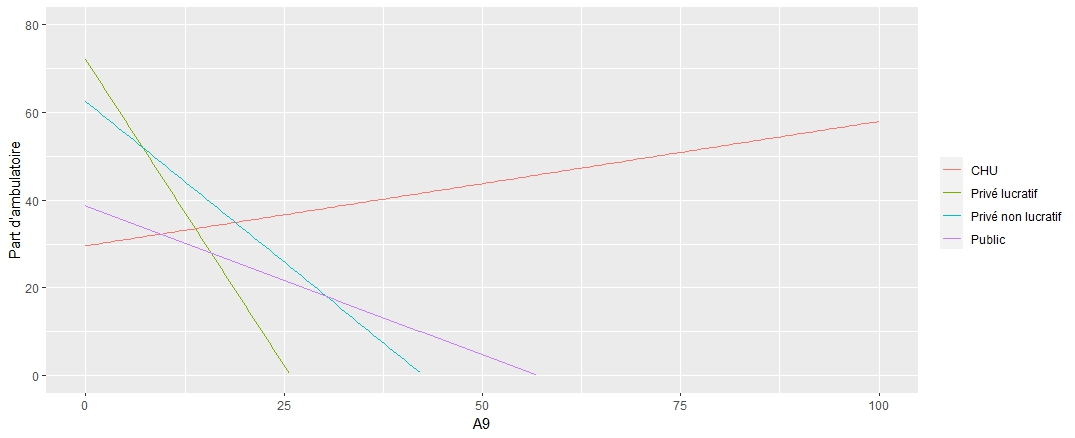
\includegraphics[scale=0.7]{Images/A9_inter.jpeg}
    \label{inter_A9}
\end{figure}

Points d'intersection (A9, Part d'ambulatoire):

\begin{itemize}
    \item CHU - Privé lucratif : $(13.8104,33.48992)$
    \item CHU - Privé non lucratif : $(18.85063,34.92148)$
    \item CHU - Public : $(9.504745,32.26701)$
    \item Privé lucratif - Privé non lucratif : 
    $(7.167806,52.07721)$
    \item Privé lucratif - Public : $(15.76718,28.01446)$
    \item Privé non lucratif - Public : $(30.25274,18.17797)$
\end{itemize}

\bigskip
\clearpage

Comme énoncé en sous-partie \ref{var_controle}, on va tester si la combinaison de la variable \textit{A9} avec la tarification permet d'améliorer le contrôle, en passant outre le problème d'agrégation de \textit{A9} au niveau des établissements, voir tableau \ref{reg_A9*tarif}.

On ne teste qu'avec la régression \ref{eqn:cat}, on observe que les résultats n'ont que très peu évolué par rapport à la régression \ref{eqn:equation_base}, de plus, le R\up{2} ajusté est plus faible par rapport au modèle avec un simple contrôle par \textit{A9}. L'utilisation seule de \textit{A9*tarification} ne permet pas un contrôle optimal.\\


\begin{table}[!htbp] \centering 
  \caption{Modèles de base avec contrôle par A9*tarification} 
  \label{reg_A9*tarif} 
\begin{tabular}{@{\extracolsep{5pt}}lD{.}{.}{-3} D{.}{.}{-3} D{.}{.}{-3} } 
\\[-1.8ex]\hline 
\hline \\[-1.8ex] 
 & \multicolumn{3}{c}{\textit{Dependent variable:}} \\ 
\cline{2-4} 
\\[-1.8ex] & \multicolumn{3}{c}{Pourcentage d'ambulatoire} \\ 
 & \multicolumn{1}{c}{default} & \multicolumn{1}{c}{robust} & \multicolumn{1}{c}{robust and clustered} \\ 
\\[-1.8ex] & \multicolumn{1}{c}{(1)} & \multicolumn{1}{c}{(2)} & \multicolumn{1}{c}{(3)}\\ 
\hline \\[-1.8ex] 
 Privé lucratif & 29.217^{***} & 29.217^{***} & 29.217^{***} \\ 
  & (0.095) & (0.119) & (0.223) \\ 
  Privé non lucratif & 19.049^{***} & 19.049^{***} & 19.049^{***} \\ 
  & (0.142) & (0.180) & (0.336) \\ 
  Public & 1.370^{***} & 1.370^{***} & 1.370^{***} \\ 
  & (0.109) & (0.118) & (0.221) \\ 
  A9*tarification & -0.004^{***} & -0.004^{***} & -0.004^{***} \\ 
  & (0.00005) & (0.00005) & (0.0001) \\ 
  Constant & 35.504^{***} & 35.504^{***} & 35.504^{***} \\ 
  & (0.084) & (0.102) & (0.193) \\ 
 \hline \\[-1.8ex] 
Observations & \multicolumn{1}{c}{669,249} & \multicolumn{1}{c}{669,249} & \multicolumn{1}{c}{669,249} \\ 
R$^{2}$ & \multicolumn{1}{c}{0.202} & \multicolumn{1}{c}{0.202} & \multicolumn{1}{c}{0.202} \\ 
Adjusted R$^{2}$ & \multicolumn{1}{c}{0.202} & \multicolumn{1}{c}{0.202} & \multicolumn{1}{c}{0.202} \\ 
Residual Std. Error (df = 669244) & \multicolumn{1}{c}{354.370} & \multicolumn{1}{c}{354.370} & \multicolumn{1}{c}{354.370} \\ 
F Statistic (df = 4; 669244) & \multicolumn{1}{c}{42,364.750$^{***}$} & \multicolumn{1}{c}{42,364.750$^{***}$} & \multicolumn{1}{c}{42,364.750$^{***}$} \\ 
\hline 
\hline \\[-1.8ex] 
\end{tabular}
\end{table}

Plutôt que de combiner la variable \textit{A9} avec la tarification des actes, on peut juste ajouter cette dernière en tant que variable de contrôle à part entière, voit tableau \ref{reg_A9_tarif}. On constate que les  le coefficient correspondant à la tarification de l'acte est négatif, ainsi, plus un acte aura un tarif élevé, moins il aura tendance à être pris en charge en ambulatoire. Cela peut être interprété comme le fait que la tarification d'un acte reflète son ampleur (pour les actes à tarification non nulle).

\clearpage




\begin{table}[!htbp] \centering 
  \caption{Modèles de base avec contrôle par A9 et tarification} 
  \label{reg_A9_tarif} 
\begin{tabular}{@{\extracolsep{5pt}}lD{.}{.}{-3} D{.}{.}{-3} D{.}{.}{-3} } 
\\[-1.8ex]\hline 
\hline \\[-1.8ex] 
 & \multicolumn{3}{c}{\textit{Dependent variable:}} \\ 
\cline{2-4} 
\\[-1.8ex] & \multicolumn{3}{c}{Pourcentage d'ambulatoire} \\ 
 & \multicolumn{1}{c}{default} & \multicolumn{1}{c}{robust} & \multicolumn{1}{c}{robust and clustered} \\ 
\\[-1.8ex] & \multicolumn{1}{c}{(1)} & \multicolumn{1}{c}{(2)} & \multicolumn{1}{c}{(3)}\\ 
\hline \\[-1.8ex] 
 Privé lucratif & 20.260^{***} & 20.260^{***} & 20.260^{***} \\ 
  & (0.126) & (0.149) & (0.274) \\ 
  Privé non lucratif & 16.384^{***} & 16.384^{***} & 16.384^{***} \\ 
  & (0.142) & (0.179) & (0.333) \\ 
  Public & 3.993^{***} & 3.993^{***} & 3.993^{***} \\ 
  & (0.110) & (0.121) & (0.226) \\ 
  A9 & -1.440^{***} & -1.440^{***} & -1.440^{***} \\ 
  & (0.011) & (0.012) & (0.021) \\ 
  tarification & -0.036^{***} & -0.036^{***} & -0.036^{***} \\ 
  & (0.0004) & (0.0005) & (0.001) \\ 
  Constant & 51.467^{***} & 51.467^{***} & 51.467^{***} \\ 
  & (0.148) & (0.171) & (0.309) \\ 
 \hline \\[-1.8ex] 
Observations & \multicolumn{1}{c}{669,249} & \multicolumn{1}{c}{669,249} & \multicolumn{1}{c}{669,249} \\ 
R$^{2}$ & \multicolumn{1}{c}{0.223} & \multicolumn{1}{c}{0.223} & \multicolumn{1}{c}{0.223} \\ 
Adjusted R$^{2}$ & \multicolumn{1}{c}{0.223} & \multicolumn{1}{c}{0.223} & \multicolumn{1}{c}{0.223} \\ 
Residual Std. Error (df = 669243) & \multicolumn{1}{c}{349.644} & \multicolumn{1}{c}{349.644} & \multicolumn{1}{c}{349.644} \\ 
F Statistic (df = 5; 669243) & \multicolumn{1}{c}{38,457.400$^{***}$} & \multicolumn{1}{c}{38,457.400$^{***}$} & \multicolumn{1}{c}{38,457.400$^{***}$} \\ 
\hline 
\hline \\[-1.8ex] 
\textit{Note:}  & \multicolumn{3}{r}{$^{*}$p$<$0.1; $^{**}$p$<$0.05; $^{***}$p$<$0.01} \\ 
\end{tabular} 
\end{table} 



L'utilisation de \textit{A9}, de la tarification des actes et de leur interaction permet cependant d'obtenir des résultats encore plus pertinents que précédemment, notamment du point de vue des critères de sélection (augmentation du R\up{2} ajusté et diminution du AIC et du BIC), les estimations sont données dans la table \ref{reg_A9_tar_int}. Le terme d'interaction des variables de contrôle permet de corriger les effets des deux variables : \textit{A9} est agrégée au niveau d'un établissement, il ne s'agit que d'une moyenne, et la tarification ne traduit pas forcément la sévérité des actes effectués (les actes à tarification nulle par exemple). 

\begin{equation} \label{eqn:controle}
    \left\{
    \begin{array}{ll}
        Y^c_i = Y_i + \beta_{A9}.A9_i + \beta_{tar}.tarification_i + \beta_{A9*tar}.A9_i.tarification_i\\
        Y_i \text{  donné par l'équation \ref{eqn:equation_base}, \ref{eqn:cat} ou \ref{eqn:annee}}
    \end{array}
\right.
\end{equation}

\bigskip

L'ajout du terme d'interaction permet essentiellement de corriger la constante qui, dans le modèle de base, correspond à la moyenne de la part d'ambulatoire dans les CHU. L'effet de cette variable de contrôle est moindre pour les autres établissements, ce qui indique que ce sont bien les CHU qui ont tendance à prendre en charge les cas les plus sévères, nécessitant une prise en charge plus longue.

Finalement, grâce à la table \ref{reg_A9_tar_int}, à sévérité d'acte égale par ailleurs, les hôpitaux privés traitent plus de cas en ambulatoire (lucratif : 74.35\%, non-lucratif : 70.23\%) que les hôpitaux publics (CHU : 53.79\%, non-CHU : 57.70\%). On constate cependant des différences assez faibles au sein des hôpitaux publics et au sein des hôpitaux privés.\\



\begin{table}[!htbp] \centering 
  \caption{Modèles de base avec contrôle par A9 et tarification (+interaction)} 
  \label{reg_A9_tar_int} 
\begin{tabular}{@{\extracolsep{5pt}}lD{.}{.}{-3} D{.}{.}{-3} D{.}{.}{-3} } 
\\[-1.8ex]\hline 
\hline \\[-1.8ex] 
 & \multicolumn{3}{c}{\textit{Dependent variable:}} \\ 
\cline{2-4} 
\\[-1.8ex] & \multicolumn{3}{c}{Pourcentage d'ambulatoire} \\ 
 & \multicolumn{1}{c}{default} & \multicolumn{1}{c}{robust} & \multicolumn{1}{c}{robust and clustered} \\ 
\\[-1.8ex] & \multicolumn{1}{c}{(1)} & \multicolumn{1}{c}{(2)} & \multicolumn{1}{c}{(3)}\\ 
\hline \\[-1.8ex] 
 Privé lucratif & 20.523^{***} & 20.523^{***} & 20.523^{***} \\ 
  & (0.126) & (0.155) & (0.284) \\ 
  Privé non lucratif & 16.413^{***} & 16.413^{***} & 16.413^{***} \\ 
  & (0.142) & (0.180) & (0.335) \\ 
  Public & 3.918^{***} & 3.918^{***} & 3.918^{***} \\ 
  & (0.109) & (0.121) & (0.226) \\ 
  A9 & -1.779^{***} & -1.779^{***} & -1.779^{***} \\ 
  & (0.013) & (0.014) & (0.025) \\ 
  tarification & -0.069^{***} & -0.069^{***} & -0.069^{***} \\ 
  & (0.001) & (0.001) & (0.001) \\ 
  A9*tarification & 0.005^{***} & 0.005^{***} & 0.005^{***} \\ 
  & (0.0001) & (0.0001) & (0.0002) \\ 
  Constant & 53.839^{***} & 53.839^{***} & 53.839^{***} \\ 
  & (0.154) & (0.182) & (0.330) \\ 
 \hline \\[-1.8ex] 
Observations & \multicolumn{1}{c}{669,249} & \multicolumn{1}{c}{669,249} & \multicolumn{1}{c}{669,249} \\ 
R$^{2}$ & \multicolumn{1}{c}{0.227} & \multicolumn{1}{c}{0.227} & \multicolumn{1}{c}{0.227} \\ 
Adjusted R$^{2}$ & \multicolumn{1}{c}{0.227} & \multicolumn{1}{c}{0.227} & \multicolumn{1}{c}{0.227} \\ 
Residual Std. Error (df = 669242) & \multicolumn{1}{c}{348.861} & \multicolumn{1}{c}{348.861} & \multicolumn{1}{c}{348.861} \\ 
F Statistic (df = 6; 669242) & \multicolumn{1}{c}{32,693.080$^{***}$} & \multicolumn{1}{c}{32,693.080$^{***}$} & \multicolumn{1}{c}{32,693.080$^{***}$} \\ 
\hline 
\hline \\[-1.8ex] 
\textit{Note:}  & \multicolumn{3}{r}{$^{*}$p$<$0.1; $^{**}$p$<$0.05; $^{***}$p$<$0.01} \\ 
\end{tabular} 
\end{table} 

\begin{table}[!htbp] \centering 
\begin{tabular}{@{\extracolsep{5pt}}lD{.}{.}{-3} D{.}{.}{-3} D{.}{.}{-3} } 
\\[-1.8ex]\hline 
\hline \\[-1.8ex] 
 & \multicolumn{3}{c}{\textit{Dependent variable:}} \\ 
\cline{2-4} 
\\[-1.8ex] & \multicolumn{3}{c}{Pourcentage d'ambulatoire} \\ 
 & \multicolumn{1}{c}{default} & \multicolumn{1}{c}{robust} & \multicolumn{1}{c}{robust and clustered} \\ 
\\[-1.8ex] & \multicolumn{1}{c}{(1)} & \multicolumn{1}{c}{(2)} & \multicolumn{1}{c}{(3)}\\ 
\hline \\[-1.8ex] 
 2016 & 1.981^{***} & 1.981^{***} & 1.981^{***} \\ 
  & (0.116) & (0.138) & (0.078) \\ 
  2017 & 4.180^{***} & 4.180^{***} & 4.180^{***} \\ 
  & (0.115) & (0.138) & (0.087) \\ 
  2018 & 6.309^{***} & 6.309^{***} & 6.309^{***} \\ 
  & (0.114) & (0.138) & (0.094) \\ 
  2019 & 7.311^{***} & 7.311^{***} & 7.311^{***} \\ 
  & (0.114) & (0.138) & (0.098) \\ 
  A9 & -3.007^{***} & -3.007^{***} & -3.007^{***} \\ 
  & (0.009) & (0.014) & (0.027) \\ 
  tarification & -0.062^{***} & -0.062^{***} & -0.062^{***} \\ 
  & (0.001) & (0.001) & (0.002) \\ 
  A9*tarification & 0.004^{***} & 0.004^{***} & 0.004^{***} \\ 
  & (0.0001) & (0.0001) & (0.0002) \\ 
  Constant & 71.039^{***} & 71.039^{***} & 71.039^{***} \\ 
  & (0.115) & (0.167) & (0.270) \\ 
 \hline \\[-1.8ex] 
Observations & \multicolumn{1}{c}{669,249} & \multicolumn{1}{c}{669,249} & \multicolumn{1}{c}{669,249} \\ 
R$^{2}$ & \multicolumn{1}{c}{0.199} & \multicolumn{1}{c}{0.199} & \multicolumn{1}{c}{0.199} \\ 
Adjusted R$^{2}$ & \multicolumn{1}{c}{0.199} & \multicolumn{1}{c}{0.199} & \multicolumn{1}{c}{0.199} \\ 
Residual Std. Error (df = 669241) & \multicolumn{1}{c}{354.958} & \multicolumn{1}{c}{354.958} & \multicolumn{1}{c}{354.958} \\ 
F Statistic (df = 7; 669241) & \multicolumn{1}{c}{23,812.700$^{***}$} & \multicolumn{1}{c}{23,812.700$^{***}$} & \multicolumn{1}{c}{23,812.700$^{***}$} \\ 
\hline 
\hline \\[-1.8ex] 
\textit{Note:}  & \multicolumn{3}{r}{$^{*}$p$<$0.1; $^{**}$p$<$0.05; $^{***}$p$<$0.01} \\
\end{tabular} 
\end{table}

\begin{table}[!htbp] \centering  
\scalebox{0.8}{
\begin{tabular}{@{\extracolsep{5pt}}lD{.}{.}{-3} D{.}{.}{-3} D{.}{.}{-3} } 
\\[-1.8ex]\hline 
\hline \\[-1.8ex] 
 & \multicolumn{3}{c}{\textit{Dependent variable:}} \\ 
\cline{2-4} 
\\[-1.8ex] & \multicolumn{3}{c}{Pourcentage d'ambulatoire} \\ 
 & \multicolumn{1}{c}{default} & \multicolumn{1}{c}{robust} & \multicolumn{1}{c}{robust and clustered} \\ 
\\[-1.8ex] & \multicolumn{1}{c}{(1)} & \multicolumn{1}{c}{(2)} & \multicolumn{1}{c}{(3)}\\ 
\hline \\[-1.8ex] 
 Privé lucratif & 20.234^{***} & 20.234^{***} & 20.234^{***} \\ 
  & (0.221) & (0.266) & (0.307) \\ 
  Privé non lucratif & 15.251^{***} & 15.251^{***} & 15.251^{***} \\ 
  & (0.321) & (0.389) & (0.392) \\ 
  Public & 3.053^{***} & 3.053^{***} & 3.053^{***} \\ 
  & (0.242) & (0.250) & (0.252) \\ 
  2016 & 1.653^{***} & 1.653^{***} & 1.653^{***} \\ 
  & (0.235) & (0.271) & (0.142) \\ 
  2017 & 3.385^{***} & 3.385^{***} & 3.385^{***} \\ 
  & (0.235) & (0.275) & (0.164) \\ 
  2018 & 5.441^{***} & 5.441^{***} & 5.441^{***} \\ 
  & (0.234) & (0.279) & (0.181) \\ 
  2019 & 6.447^{***} & 6.447^{***} & 6.447^{***} \\ 
  & (0.234) & (0.282) & (0.193) \\ 
  A9 & -1.830^{***} & -1.830^{***} & -1.830^{***} \\ 
  & (0.013) & (0.015) & (0.026) \\ 
  tarification & -0.069^{***} & -0.069^{***} & -0.069^{***} \\ 
  & (0.001) & (0.001) & (0.001) \\ 
  Privé lucratif*2016 & 0.207 & 0.207 & 0.207 \\ 
  & (0.288) & (0.353) & (0.193) \\ 
  Privé non lucratif*2016 & -0.033 & -0.033 & -0.033 \\ 
  & (0.453) & (0.557) & (0.316) \\ 
  Public*2016 & 0.728^{**} & 0.728^{**} & 0.728^{***} \\ 
  & (0.340) & (0.357) & (0.197) \\ 
  Privé lucratif*2017 & 0.151 & 0.151 & 0.151 \\ 
  & (0.286) & (0.355) & (0.217) \\ 
  Privé non lucratif*2017 & 1.549^{***} & 1.549^{***} & 1.549^{***} \\ 
  & (0.445) & (0.555) & (0.356) \\ 
  Public*2017 & 1.192^{***} & 1.192^{***} & 1.192^{***} \\ 
  & (0.338) & (0.361) & (0.224) \\ 
  Privé lucratif*2018 & -0.295 & -0.295 & -0.295 \\ 
  & (0.285) & (0.358) & (0.236) \\ 
  Privé non lucratif*2018 & 1.494^{***} & 1.494^{***} & 1.494^{***} \\ 
  & (0.442) & (0.557) & (0.378) \\ 
  Public*2018 & 1.374^{***} & 1.374^{***} & 1.374^{***} \\ 
  & (0.338) & (0.367) & (0.244) \\ 
  Privé lucratif*2019 & -0.633^{**} & -0.633^{*} & -0.633^{**} \\ 
  & (0.285) & (0.359) & (0.249) \\ 
  Privé non lucratif*2019 & 1.501^{***} & 1.501^{***} & 1.501^{***} \\ 
  & (0.440) & (0.556) & (0.398) \\ 
  Public*2019 & 1.595^{***} & 1.595^{***} & 1.595^{***} \\ 
  & (0.337) & (0.370) & (0.260) \\ 
  A9*tarification & 0.005^{***} & 0.005^{***} & 0.005^{***} \\ 
  & (0.0001) & (0.0001) & (0.0002) \\ 
  Constant & 51.009^{***} & 51.009^{***} & 51.009^{***} \\ 
  & (0.214) & (0.246) & (0.341) \\ 
 \hline \\[-1.8ex] 
Observations & \multicolumn{1}{c}{669,249} & \multicolumn{1}{c}{669,249} & \multicolumn{1}{c}{669,249} \\ 
R$^{2}$ & \multicolumn{1}{c}{0.232} & \multicolumn{1}{c}{0.232} & \multicolumn{1}{c}{0.232} \\ 
Adjusted R$^{2}$ & \multicolumn{1}{c}{0.232} & \multicolumn{1}{c}{0.232} & \multicolumn{1}{c}{0.232} \\ 
Residual Std. Error (df = 669226) & \multicolumn{1}{c}{347.619} & \multicolumn{1}{c}{347.619} & \multicolumn{1}{c}{347.619} \\ 
F Statistic (df = 22; 669226) & \multicolumn{1}{c}{9,198.750$^{***}$} & \multicolumn{1}{c}{9,198.750$^{***}$} & \multicolumn{1}{c}{9,198.750$^{***}$} \\ 
\hline 
\hline \\[-1.8ex] 
\end{tabular} 
}
\end{table} 

\clearpage

De la même manière, on peut rajouter les variables \textit{A10} et \textit{A11} dans la régression \ref{eqn:controle}, elles traduisent de l'importance des activités d'enseignement et de recherche qui sont particulièrement présentes dans les CHU (voir table \ref{reg_controle_A1}). On observe un impact assez important sur les variables donnant la catégorie de l'établissement, il s'agit donc d'un contrôle pertinent. \textit{A10} et \textit{A11} ont bien un coefficient  négatif, ce qui traduit que les activités d'enseignement et de recherche ont bien un impact négatif sur la part d'ambulatoire. Ces variables corrigent essentiellement la constante puisque ces activités concernent surtout les CHU. On constate que, désormais, en prenant en compte ces aspects, il n'y a  plus de différence significative entre les CHU et les autres hôpitaux publics.\\


\begin{table}[!htbp] \centering 
  \caption{Modèle \ref{eqn:controle} avec contrôle par A10 et A11} 
  \label{reg_controle_A1} 
\begin{tabular}{@{\extracolsep{5pt}}lD{.}{.}{-3} D{.}{.}{-3} D{.}{.}{-3} } 
\\[-1.8ex]\hline 
\hline \\[-1.8ex] 
 & \multicolumn{3}{c}{\textit{Dependent variable:}} \\ 
\cline{2-4} 
\\[-1.8ex] & \multicolumn{3}{c}{Pourcentage d'ambulatoire} \\ 
 & \multicolumn{1}{c}{default} & \multicolumn{1}{c}{robust} & \multicolumn{1}{c}{robust and clustered} \\ 
\\[-1.8ex] & \multicolumn{1}{c}{(1)} & \multicolumn{1}{c}{(2)} & \multicolumn{1}{c}{(3)}\\ 
\hline \\[-1.8ex] 
 Privé lucratif & 16.573^{***} & 16.573^{***} & 16.573^{***} \\ 
  & (0.209) & (0.250) & (0.439) \\ 
  Privé non lucratif & 13.431^{***} & 13.431^{***} & 13.431^{***} \\ 
  & (0.200) & (0.238) & (0.427) \\ 
  Public & 0.175 & 0.175 & 0.175 \\ 
  & (0.192) & (0.222) & (0.389) \\ 
  A9 & -1.772^{***} & -1.772^{***} & -1.772^{***} \\ 
  & (0.013) & (0.014) & (0.025) \\ 
  tarification & -0.069^{***} & -0.069^{***} & -0.069^{***} \\ 
  & (0.001) & (0.001) & (0.001) \\ 
  A10 & -2.809^{***} & -2.809^{***} & -2.809^{***} \\ 
  & (0.135) & (0.157) & (0.272) \\ 
  A11 & -0.466^{***} & -0.466^{***} & -0.466^{***} \\ 
  & (0.068) & (0.099) & (0.167) \\ 
  A9*tarification & 0.005^{***} & 0.005^{***} & 0.005^{***} \\ 
  & (0.0001) & (0.0001) & (0.0002) \\ 
  Constant & 57.784^{***} & 57.784^{***} & 57.784^{***} \\ 
  & (0.227) & (0.270) & (0.473) \\ 
 \hline \\[-1.8ex] 
Observations & \multicolumn{1}{c}{669,249} & \multicolumn{1}{c}{669,249} & \multicolumn{1}{c}{669,249} \\ 
R$^{2}$ & \multicolumn{1}{c}{0.227} & \multicolumn{1}{c}{0.227} & \multicolumn{1}{c}{0.227} \\ 
Adjusted R$^{2}$ & \multicolumn{1}{c}{0.227} & \multicolumn{1}{c}{0.227} & \multicolumn{1}{c}{0.227} \\ 
Residual Std. Error (df = 669240) & \multicolumn{1}{c}{348.716} & \multicolumn{1}{c}{348.716} & \multicolumn{1}{c}{348.716} \\ 
F Statistic (df = 8; 669240) & \multicolumn{1}{c}{24,610.520$^{***}$} & \multicolumn{1}{c}{24,610.520$^{***}$} & \multicolumn{1}{c}{24,610.520$^{***}$} \\ 
\hline 
\hline \\[-1.8ex] 
\textit{Note:}  & \multicolumn{3}{r}{$^{*}$p$<$0.1; $^{**}$p$<$0.05; $^{***}$p$<$0.01} \\ 
\end{tabular} 
\end{table} 

\bigskip

Comme précédemment, on procède à un contrôle par \textit{A10}, \textit{A11} et leur interaction (tableau \ref{reg_controle_A1_inter}). En général, l'enseignement et la recherche vont de pair, en particulier au sein des CHU grâce aux enseignants-chercheurs. On effectue donc la régression suivante :

\begin{equation} \label{eqn:controle_A1}
    \left\{
    \begin{array}{ll}
        Y^{c_2}_i = Y^c_i + \beta_{A10}.A10_i + \beta_{A11}.A11_i + \beta_{A10*A11}.A10_i.A11_i\\
        Y^c_i \text{  donné par l'équation \ref{eqn:controle}}
    \end{array}
\right.
\end{equation}

\bigskip



\begin{table}[!htbp] \centering 
  \caption{Modèle \ref{eqn:controle} avec contrôle par A10 et A11 (+interaction)} 
  \label{reg_controle_A1_inter} 
\begin{tabular}{@{\extracolsep{5pt}}lD{.}{.}{-3} D{.}{.}{-3} D{.}{.}{-3} } 
\\[-1.8ex]\hline 
\hline \\[-1.8ex] 
 & \multicolumn{3}{c}{\textit{Dependent variable:}} \\ 
\cline{2-4} 
\\[-1.8ex] & \multicolumn{3}{c}{Pourcentage d'ambulatoire} \\ 
 & \multicolumn{1}{c}{default} & \multicolumn{1}{c}{robust} & \multicolumn{1}{c}{robust and clustered} \\ 
\\[-1.8ex] & \multicolumn{1}{c}{(1)} & \multicolumn{1}{c}{(2)} & \multicolumn{1}{c}{(3)}\\ 
\hline \\[-1.8ex] 
 Privé lucratif & 16.260^{***} & 16.260^{***} & 16.260^{***} \\ 
  & (0.211) & (0.252) & (0.443) \\ 
  Privé non lucratif & 13.271^{***} & 13.271^{***} & 13.271^{***} \\ 
  & (0.200) & (0.239) & (0.429) \\ 
  Public & 0.098 & 0.098 & 0.098 \\ 
  & (0.192) & (0.222) & (0.389) \\ 
  A9 & -1.781^{***} & -1.781^{***} & -1.781^{***} \\ 
  & (0.013) & (0.014) & (0.025) \\ 
  tarification & -0.069^{***} & -0.069^{***} & -0.069^{***} \\ 
  & (0.001) & (0.001) & (0.001) \\ 
  A10 & -4.619^{***} & -4.619^{***} & -4.619^{***} \\ 
  & (0.207) & (0.247) & (0.442) \\ 
  A11 & -0.875^{***} & -0.875^{***} & -0.875^{***} \\ 
  & (0.077) & (0.115) & (0.192) \\ 
  A9*tarification & 0.005^{***} & 0.005^{***} & 0.005^{***} \\ 
  & (0.0001) & (0.0001) & (0.0002) \\ 
  A10*A11 & 1.742^{***} & 1.742^{***} & 1.742^{***} \\ 
  & (0.151) & (0.195) & (0.344) \\ 
  Constant & 58.137^{***} & 58.137^{***} & 58.137^{***} \\ 
  & (0.229) & (0.272) & (0.477) \\ 
 \hline \\[-1.8ex] 
Observations & \multicolumn{1}{c}{669,249} & \multicolumn{1}{c}{669,249} & \multicolumn{1}{c}{669,249} \\ 
R$^{2}$ & \multicolumn{1}{c}{0.227} & \multicolumn{1}{c}{0.227} & \multicolumn{1}{c}{0.227} \\ 
Adjusted R$^{2}$ & \multicolumn{1}{c}{0.227} & \multicolumn{1}{c}{0.227} & \multicolumn{1}{c}{0.227} \\ 
Residual Std. Error (df = 669239) & \multicolumn{1}{c}{348.681} & \multicolumn{1}{c}{348.681} & \multicolumn{1}{c}{348.681} \\ 
F Statistic (df = 9; 669239) & \multicolumn{1}{c}{21,895.070$^{***}$} & \multicolumn{1}{c}{21,895.070$^{***}$} & \multicolumn{1}{c}{21,895.070$^{***}$} \\ 
\hline 
\hline \\[-1.8ex] 
\textit{Note:}  & \multicolumn{3}{r}{$^{*}$p$<$0.1; $^{**}$p$<$0.05; $^{***}$p$<$0.01} \\ 
\end{tabular} 
\end{table} 

Les estimations de cette régression sont données dans le tableau \ref{reg_controle_A1_inter}. Ici, le coefficient de la variable d'interaction est significatif et négatif, elle permet donc de corriger le contrôle de \textit{A10} et de \textit{A11}. Cependant, l'ajout de ce terme a un impact assez faible sur les autres variables.\\

On observe qu'avec ces contrôles, la part moyenne d'actes effectués en ambulatoire est plus importante pour toutes les catégories d'établissements, l'écart entre les CHU et hôpitaux publics autres n'est pas significatif. Il y a tout de même un écart significatif entre les hôpitaux publics et les établissements privées.

\begin{table}[!htbp] \centering  
\begin{tabular}{@{\extracolsep{5pt}}lD{.}{.}{-3} D{.}{.}{-3} D{.}{.}{-3} } 
\\[-1.8ex]\hline 
\hline \\[-1.8ex] 
 & \multicolumn{3}{c}{\textit{Dependent variable:}} \\ 
\cline{2-4} 
\\[-1.8ex] & \multicolumn{3}{c}{Pourcentage d'ambulatoire} \\ 
 & \multicolumn{1}{c}{default} & \multicolumn{1}{c}{robust} & \multicolumn{1}{c}{robust and clustered} \\ 
\\[-1.8ex] & \multicolumn{1}{c}{(1)} & \multicolumn{1}{c}{(2)} & \multicolumn{1}{c}{(3)}\\ 
\hline \\[-1.8ex] 
 2016 & 1.903^{***} & 1.903^{***} & 1.903^{***} \\ 
  & (0.115) & (0.137) & (0.078) \\ 
  2017 & 4.219^{***} & 4.219^{***} & 4.219^{***} \\ 
  & (0.114) & (0.138) & (0.087) \\ 
  2018 & 6.303^{***} & 6.303^{***} & 6.303^{***} \\ 
  & (0.113) & (0.138) & (0.093) \\ 
  2019 & 7.290^{***} & 7.290^{***} & 7.290^{***} \\ 
  & (0.113) & (0.138) & (0.098) \\ 
  A9 & -2.701^{***} & -2.701^{***} & -2.701^{***} \\ 
  & (0.010) & (0.014) & (0.026) \\ 
  tarification & -0.066^{***} & -0.066^{***} & -0.066^{***} \\ 
  & (0.001) & (0.001) & (0.002) \\ 
  A10 & -12.468^{***} & -12.468^{***} & -12.468^{***} \\ 
  & (0.167) & (0.206) & (0.374) \\ 
  A11 & -0.734^{***} & -0.734^{***} & -0.734^{***} \\ 
  & (0.071) & (0.106) & (0.181) \\ 
  A9*tarification & 0.004^{***} & 0.004^{***} & 0.004^{***} \\ 
  & (0.0001) & (0.0001) & (0.0002) \\ 
  A10*A11 & 4.389^{***} & 4.389^{***} & 4.389^{***} \\ 
  & (0.150) & (0.193) & (0.341) \\ 
  Constant & 71.586^{***} & 71.586^{***} & 71.586^{***} \\ 
  & (0.114) & (0.164) & (0.262) \\ 
 \hline \\[-1.8ex] 
Observations & \multicolumn{1}{c}{669,249} & \multicolumn{1}{c}{669,249} & \multicolumn{1}{c}{669,249} \\ 
R$^{2}$ & \multicolumn{1}{c}{0.217} & \multicolumn{1}{c}{0.217} & \multicolumn{1}{c}{0.217} \\ 
Adjusted R$^{2}$ & \multicolumn{1}{c}{0.217} & \multicolumn{1}{c}{0.217} & \multicolumn{1}{c}{0.217} \\ 
Residual Std. Error (df = 669238) & \multicolumn{1}{c}{350.964} & \multicolumn{1}{c}{350.964} & \multicolumn{1}{c}{350.964} \\ 
F Statistic (df = 10; 669238) & \multicolumn{1}{c}{18,582.610$^{***}$} & \multicolumn{1}{c}{18,582.610$^{***}$} & \multicolumn{1}{c}{18,582.610$^{***}$} \\ 
\hline 
\hline \\[-1.8ex] 
\end{tabular} 
\end{table} 


\begin{table}[!htbp] \centering 
\scalebox{0.72}{
\begin{tabular}{@{\extracolsep{5pt}}lD{.}{.}{-3} D{.}{.}{-3} D{.}{.}{-3} } 
\\[-1.8ex]\hline 
\hline \\[-1.8ex] 
 & \multicolumn{3}{c}{\textit{Dependent variable:}} \\ 
\cline{2-4} 
\\[-1.8ex] & \multicolumn{3}{c}{Pourcentage d'ambulatoire} \\ 
 & \multicolumn{1}{c}{default} & \multicolumn{1}{c}{robust} & \multicolumn{1}{c}{robust and clustered} \\ 
\\[-1.8ex] & \multicolumn{1}{c}{(1)} & \multicolumn{1}{c}{(2)} & \multicolumn{1}{c}{(3)}\\ 
\hline \\[-1.8ex] 
 Privé lucratif & 15.420^{***} & 15.420^{***} & 15.420^{***} \\ 
  & (0.279) & (0.331) & (0.458) \\ 
  Privé non lucratif & 11.838^{***} & 11.838^{***} & 11.838^{***} \\ 
  & (0.350) & (0.416) & (0.470) \\ 
  Public & -1.338^{***} & -1.338^{***} & -1.338^{***} \\ 
  & (0.290) & (0.312) & (0.407) \\ 
  2016 & 1.478^{***} & 1.478^{***} & 1.478^{***} \\ 
  & (0.235) & (0.271) & (0.143) \\ 
  2017 & 3.455^{***} & 3.455^{***} & 3.455^{***} \\ 
  & (0.234) & (0.275) & (0.165) \\ 
  2018 & 5.530^{***} & 5.530^{***} & 5.530^{***} \\ 
  & (0.234) & (0.279) & (0.182) \\ 
  2019 & 6.540^{***} & 6.540^{***} & 6.540^{***} \\ 
  & (0.234) & (0.282) & (0.194) \\ 
  A9 & -1.832^{***} & -1.832^{***} & -1.832^{***} \\ 
  & (0.013) & (0.015) & (0.026) \\ 
  tarification & -0.069^{***} & -0.069^{***} & -0.069^{***} \\ 
  & (0.001) & (0.001) & (0.001) \\ 
  A10 & -5.071^{***} & -5.071^{***} & -5.071^{***} \\ 
  & (0.206) & (0.246) & (0.443) \\ 
  A11 & -1.119^{***} & -1.119^{***} & -1.119^{***} \\ 
  & (0.077) & (0.115) & (0.193) \\ 
  Privé lucratif*2016 & 0.382 & 0.382 & 0.382^{**} \\ 
  & (0.288) & (0.353) & (0.193) \\ 
  Privé non lucratif*2016 & -0.228 & -0.228 & -0.228 \\ 
  & (0.453) & (0.557) & (0.317) \\ 
  Public*2016 & 0.978^{***} & 0.978^{***} & 0.978^{***} \\ 
  & (0.340) & (0.357) & (0.198) \\ 
  Privé lucratif*2017 & 0.187 & 0.187 & 0.187 \\ 
  & (0.286) & (0.355) & (0.218) \\ 
  Privé non lucratif*2017 & 1.438^{***} & 1.438^{***} & 1.438^{***} \\ 
  & (0.445) & (0.555) & (0.357) \\ 
  Public*2017 & 1.249^{***} & 1.249^{***} & 1.249^{***} \\ 
  & (0.338) & (0.361) & (0.224) \\ 
  Privé lucratif*2018 & -0.357 & -0.357 & -0.357 \\ 
  & (0.285) & (0.358) & (0.236) \\ 
  Privé non lucratif*2018 & 1.531^{***} & 1.531^{***} & 1.531^{***} \\ 
  & (0.441) & (0.557) & (0.379) \\ 
  Public*2018 & 1.424^{***} & 1.424^{***} & 1.424^{***} \\ 
  & (0.337) & (0.367) & (0.245) \\ 
  Privé lucratif*2019 & -0.694^{**} & -0.694^{*} & -0.694^{***} \\ 
  & (0.285) & (0.359) & (0.250) \\ 
  Privé non lucratif*2019 & 1.656^{***} & 1.656^{***} & 1.656^{***} \\ 
  & (0.440) & (0.557) & (0.400) \\ 
  Public*2019 & 1.669^{***} & 1.669^{***} & 1.669^{***} \\ 
  & (0.337) & (0.371) & (0.261) \\ 
  A9*tarification & 0.005^{***} & 0.005^{***} & 0.005^{***} \\ 
  & (0.0001) & (0.0001) & (0.0002) \\ 
  A10*A11 & 1.947^{***} & 1.947^{***} & 1.947^{***} \\ 
  & (0.151) & (0.194) & (0.345) \\ 
  Constant & 55.834^{***} & 55.834^{***} & 55.834^{***} \\ 
  & (0.273) & (0.317) & (0.484) \\ 
 \hline \\[-1.8ex] 
Observations & \multicolumn{1}{c}{669,249} & \multicolumn{1}{c}{669,249} & \multicolumn{1}{c}{669,249} \\ 
R$^{2}$ & \multicolumn{1}{c}{0.233} & \multicolumn{1}{c}{0.233} & \multicolumn{1}{c}{0.233} \\ 
Adjusted R$^{2}$ & \multicolumn{1}{c}{0.233} & \multicolumn{1}{c}{0.233} & \multicolumn{1}{c}{0.233} \\ 
Residual Std. Error (df = 669223) & \multicolumn{1}{c}{347.389} & \multicolumn{1}{c}{347.389} & \multicolumn{1}{c}{347.389} \\ 
F Statistic (df = 25; 669223) & \multicolumn{1}{c}{8,141.247$^{***}$} & \multicolumn{1}{c}{8,141.247$^{***}$} & \multicolumn{1}{c}{8,141.247$^{***}$} \\ 
\hline 
\hline \\[-1.8ex]  
\end{tabular}
}
\end{table} 


Nous allons de nouveau effectuer une régression avec contrôle par interaction avec \textit{A9} mais en conservant les autres variables de contrôle. On va donc utiliser le modèle \ref{eqn:controle_inter}, les estimations des coefficients sont consultables dans la table \ref{controle_inter} et les courbes de la part d'actes en ambulatoire selon \textit{A9} pour chaque catégorie d'établissement sont dans la figure \ref{courbe_inter}. On observe des résultats plus pertinents que pour le modèle à interaction \ref{eqn:int}, notamment vis-à-vis des CHU pour lesquels on observe bien une diminution de la part d'actes en ambulatoire avec l'augmentation de \textit{A9}.\\


\begin{equation} \label{eqn:controle_inter}
    \left\{
    \begin{array}{ll}
        Y^{inter_2}_i = Y^{inter}_i + \beta_{tar}.tarification_i + \beta_{A9*tar}.A9_i.tarification_i +\\
        \qquad \qquad \qquad \qquad \qquad \qquad \qquad \qquad  \beta_{A10}.A10_i + \beta_{A11}.A11_i + \beta_{A10*A11}.A10_i.A11_i\\
        Y^{inter}_i \text{  donné par l'équation \ref{eqn:int}}
    \end{array}
\right.
\end{equation}

\bigskip

\begin{figure}[!ht]
    \centering
    \caption{Estimation de la part d'ambulatoire en fonction de A9 (Modèle \ref{eqn:controle_inter})}
    \label{courbe_inter}
    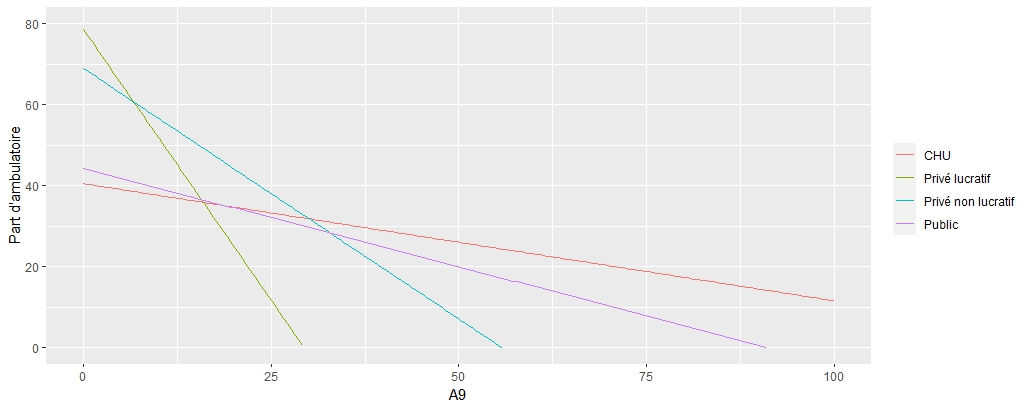
\includegraphics[scale=0.7]{Images/A9_inter_c.jpeg}
    \label{inter_A9_c}
\end{figure}


Points d'intersection (A9, Part d'ambulatoire):

\begin{itemize}
    \item CHU - Privé lucratif : $(15.94116,35.89712)$
    \item CHU - Privé non lucratif : $(30.04572,31.82359)$
    \item CHU - Public : $(19.13799,34.97384)$
    \item Privé lucratif - Privé non lucratif : $(6.652049,60.71998)$
    \item Privé lucratif - Public : $(15.65566,36.66004)$
    \item Privé non lucratif - Public : $(32.88388,28.31783)$
\end{itemize}


\begin{table}[!htbp] \centering 
  \caption{Modèle \ref{eqn:controle_inter} avec contrôle par interaction de A9} 
  \label{controle_inter} 
\begin{tabular}{@{\extracolsep{5pt}}lD{.}{.}{-3} D{.}{.}{-3} D{.}{.}{-3} } 
\\[-1.8ex]\hline 
\hline \\[-1.8ex] 
 & \multicolumn{3}{c}{\textit{Dependent variable:}} \\ 
\cline{2-4} 
\\[-1.8ex] & \multicolumn{3}{c}{Pourcentage d'ambulatoire} \\ 
 & \multicolumn{1}{c}{default} & \multicolumn{1}{c}{robust} & \multicolumn{1}{c}{robust and clustered} \\ 
\\[-1.8ex] & \multicolumn{1}{c}{(1)} & \multicolumn{1}{c}{(2)} & \multicolumn{1}{c}{(3)}\\ 
\hline \\[-1.8ex] 
 Privé lucratif & 37.995^{***} & 37.995^{***} & 37.995^{***} \\ 
  & (0.812) & (0.963) & (1.648) \\ 
  Privé non lucratif & 28.436^{***} & 28.436^{***} & 28.436^{***} \\ 
  & (0.831) & (0.975) & (1.683) \\ 
  Public & 3.740^{***} & 3.740^{***} & 3.740^{**} \\ 
  & (0.849) & (0.969) & (1.667) \\ 
  A9 & -0.289^{***} & -0.289^{***} & -0.289^{**} \\ 
  & (0.068) & (0.080) & (0.137) \\ 
  tarification & -0.073^{***} & -0.073^{***} & -0.073^{***} \\ 
  & (0.001) & (0.001) & (0.002) \\ 
  A10 & -3.298^{***} & -3.298^{***} & -3.298^{***} \\ 
  & (0.209) & (0.249) & (0.445) \\ 
  A11 & -0.766^{***} & -0.766^{***} & -0.766^{***} \\ 
  & (0.077) & (0.115) & (0.191) \\ 
  Privé lucratif*A9 & -2.672^{***} & -2.672^{***} & -2.672^{***} \\ 
  & (0.070) & (0.091) & (0.154) \\ 
  Privé non lucratif*A9 & -1.235^{***} & -1.235^{***} & -1.235^{***} \\ 
  & (0.071) & (0.082) & (0.143) \\ 
  Public*A9 & -0.484^{***} & -0.484^{***} & -0.484^{***} \\ 
  & (0.071) & (0.081) & (0.139) \\ 
  A9*tarification & 0.005^{***} & 0.005^{***} & 0.005^{***} \\ 
  & (0.0001) & (0.0001) & (0.0002) \\ 
  A10*A11 & 0.928^{***} & 0.928^{***} & 0.928^{***} \\ 
  & (0.151) & (0.195) & (0.344) \\ 
  Constant & 40.501^{***} & 40.501^{***} & 40.501^{***} \\ 
  & (0.810) & (0.953) & (1.633) \\ 
 \hline \\[-1.8ex] 
Observations & \multicolumn{1}{c}{669,249} & \multicolumn{1}{c}{669,249} & \multicolumn{1}{c}{669,249} \\ 
R$^{2}$ & \multicolumn{1}{c}{0.236} & \multicolumn{1}{c}{0.236} & \multicolumn{1}{c}{0.236} \\ 
Adjusted R$^{2}$ & \multicolumn{1}{c}{0.236} & \multicolumn{1}{c}{0.236} & \multicolumn{1}{c}{0.236} \\ 
Residual Std. Error (df = 669236) & \multicolumn{1}{c}{346.818} & \multicolumn{1}{c}{346.818} & \multicolumn{1}{c}{346.818} \\ 
F Statistic (df = 12; 669236) & \multicolumn{1}{c}{17,199.460$^{***}$} & \multicolumn{1}{c}{17,199.460$^{***}$} & \multicolumn{1}{c}{17,199.460$^{***}$} \\ 
\hline 
\hline \\[-1.8ex] 
\textit{Note:}  & \multicolumn{3}{r}{$^{*}$p$<$0.1; $^{**}$p$<$0.05; $^{***}$p$<$0.01} \\ 
\end{tabular} 
\end{table}


\clearpage

\subsection{Actes chirurgicaux sélectionnés}

Dans cette partie nous allons nous concentrer sur les actes chirurgicaux parmi les actes sélectionnés dans la base de données CCAM.

\begin{table}[ht]
\centering
\caption{Pourcentage moyen d'actes de chirurgie effectués en ambulatoire (\%)} 
\label{part_ambu_tabu_chir}
\begin{tabular}{r|cccc|c}
  \hline
 & CHU & Privé lucratif & Privé non lucratif & Public & Total \\ 
  \hline
2015 & 32.10 & 58.61 & 53.79 & 39.10 & 50.33 \\ 
  2016 & 35.63 & 62.15 & 56.32 & 43.14 & 53.68 \\ 
  2017 & 38.84 & 64.31 & 59.81 & 45.93 & 56.15 \\ 
  2018 & 41.76 & 66.72 & 62.24 & 49.07 & 58.83 \\ 
  2019 & 44.02 & 68.91 & 64.06 & 50.77 & 60.96 \\ 
  \hline
  Total & 38.46 & 64.10 & 59.36 & 45.66 & 55.99 \\ 
   \hline
\end{tabular}

\bigskip

\begin{tabular}{ccccc}
  \hline
Min. & 1er Qu. & Médiane & 3e Qu. & Max. \\ 
  \hline
0.00 & 30.42 & 65.04 & 84.60 & 100.00 \\ 
   \hline
\end{tabular}
\end{table}


\begin{table}[!ht]
\centering
\caption{Durée moyenne des séjours en chirurgie} 
\label{dms_tabu_chir}
\begin{tabular}{r|cccc|c}
  \hline
 & CHU & Privé lucratif & Privé non lucratif & Public & Total \\ 
  \hline
2015 & 5.68 & 1.09 & 2.08 & 3.50 & 2.34 \\ 
  2016 & 5.32 & 0.98 & 1.97 & 3.19 & 2.18 \\ 
  2017 & 5.04 & 0.91 & 1.74 & 3.00 & 2.05 \\ 
  2018 & 4.71 & 0.84 & 1.59 & 2.81 & 1.90 \\ 
  2019 & 4.53 & 0.79 & 1.52 & 2.73 & 1.81 \\
  \hline
  Total & 5.06 & 0.92 & 1.77 & 3.04 & 2.06 \\ 
   \hline
\end{tabular}

\bigskip

\begin{tabular}{ccccc}
  \hline
Min. & 1er Qu. & Médiane & 3e Qu. & Max. \\ 
  \hline
0.00 & 0.25 & 0.86 & 2.27 & 145.00 \\ 
   \hline
\end{tabular}
\end{table}

Les tableaux \ref{part_ambu_tabu_chir} et \ref{dms_tabu_chir} présentent les moyennes issues des modèles linéaires de base. De manière globale, les actes chirurgicaux ont plus tendance à être effectués en ambulatoire que l'ensemble des actes (55.99\% pour les actes chirurgicaux contre 49.05\% pour l'ensemble des actes sélectionnés).\\

Le tableau \ref{part_ambu_select_chir} présente les estimations des coefficients des modèles \ref{eqn:cat}, \ref{eqn:annee} et \ref{eqn:equation_base} qu'on a utilisé pour retrouver les moyennes conditionnelles (tableau \ref{part_ambu_tabu_chir}). On constate également que les écarts entre les catégories d'établissements ont changé de manière non monotone par rapport à l'application sur l'ensemble des actes sélectionnés (écart CHU--Privé lucratif plus faible et écart CHU--Public plus élevé).


\begin{table}[!htbp] \centering 
  \caption{Modèles de base appliqué à la part d’actes chirurgicaux en ambulatoire} 
  \label{part_ambu_select_chir} 
\begin{tabular}{@{\extracolsep{5pt}}lD{.}{.}{-3} D{.}{.}{-3} D{.}{.}{-3} } 
\\[-1.8ex]\hline 
\hline \\[-1.8ex] 
 & \multicolumn{3}{c}{\textit{Dependent variable:}} \\ 
\cline{2-4} 
\\[-1.8ex] & \multicolumn{3}{c}{Pourcentage d'ambulatoire} \\ 
 & \multicolumn{1}{c}{default} & \multicolumn{1}{c}{robust} & \multicolumn{1}{c}{robust and clustered} \\ 
\\[-1.8ex] & \multicolumn{1}{c}{(1)} & \multicolumn{1}{c}{(2)} & \multicolumn{1}{c}{(3)}\\ 
\hline \\[-1.8ex] 
 Privé lucratif & 25.634^{***} & 25.634^{***} & 25.634^{***} \\ 
  & (0.181) & (0.209) & (0.380) \\ 
  Privé non lucratif & 20.895^{***} & 20.895^{***} & 20.895^{***} \\ 
  & (0.255) & (0.319) & (0.574) \\ 
  Public & 7.199^{***} & 7.199^{***} & 7.199^{***} \\ 
  & (0.208) & (0.229) & (0.414) \\ 
  Constant & 38.464^{***} & 38.464^{***} & 38.464^{***} \\ 
  & (0.160) & (0.180) & (0.329) \\ 
 \hline \\[-1.8ex] 
Observations & \multicolumn{1}{c}{262,629} & \multicolumn{1}{c}{262,629} & \multicolumn{1}{c}{262,629} \\ 
R$^{2}$ & \multicolumn{1}{c}{0.096} & \multicolumn{1}{c}{0.096} & \multicolumn{1}{c}{0.096} \\ 
Adjusted R$^{2}$ & \multicolumn{1}{c}{0.096} & \multicolumn{1}{c}{0.096} & \multicolumn{1}{c}{0.096} \\ 
Residual Std. Error (df = 262625) & \multicolumn{1}{c}{251.683} & \multicolumn{1}{c}{251.683} & \multicolumn{1}{c}{251.683} \\ 
F Statistic (df = 3; 262625) & \multicolumn{1}{c}{9,271.625$^{***}$} & \multicolumn{1}{c}{9,271.625$^{***}$} & \multicolumn{1}{c}{9,271.625$^{***}$} \\ 
\hline 
\hline \\[-1.8ex] 
\end{tabular} 

\bigskip

\begin{tabular}{@{\extracolsep{5pt}}lD{.}{.}{-3} D{.}{.}{-3} D{.}{.}{-3} } 
\\[-1.8ex]\hline 
\hline \\[-1.8ex] 
 & \multicolumn{3}{c}{\textit{Dependent variable:}} \\ 
\cline{2-4} 
\\[-1.8ex] & \multicolumn{3}{c}{Pourcentage d'ambulatoire} \\ 
 & \multicolumn{1}{c}{default} & \multicolumn{1}{c}{robust} & \multicolumn{1}{c}{robust and clustered} \\ 
\\[-1.8ex] & \multicolumn{1}{c}{(1)} & \multicolumn{1}{c}{(2)} & \multicolumn{1}{c}{(3)}\\ 
\hline \\[-1.8ex] 
 2016 & 3.346^{***} & 3.346^{***} & 3.346^{***} \\ 
  & (0.202) & (0.236) & (0.141) \\ 
  2017 & 5.813^{***} & 5.813^{***} & 5.813^{***} \\ 
  & (0.202) & (0.236) & (0.156) \\ 
  2018 & 8.493^{***} & 8.493^{***} & 8.493^{***} \\ 
  & (0.202) & (0.236) & (0.166) \\ 
  2019 & 10.627^{***} & 10.627^{***} & 10.627^{***} \\ 
  & (0.202) & (0.235) & (0.173) \\ 
  Constant & 50.335^{***} & 50.335^{***} & 50.335^{***} \\ 
  & (0.142) & (0.165) & (0.165) \\ 
 \hline \\[-1.8ex] 
Observations & \multicolumn{1}{c}{262,629} & \multicolumn{1}{c}{262,629} & \multicolumn{1}{c}{262,629} \\ 
R$^{2}$ & \multicolumn{1}{c}{0.013} & \multicolumn{1}{c}{0.013} & \multicolumn{1}{c}{0.013} \\ 
Adjusted R$^{2}$ & \multicolumn{1}{c}{0.013} & \multicolumn{1}{c}{0.013} & \multicolumn{1}{c}{0.013} \\ 
Residual Std. Error (df = 262624) & \multicolumn{1}{c}{262.958} & \multicolumn{1}{c}{262.958} & \multicolumn{1}{c}{262.958} \\ 
F Statistic (df = 4; 262624) & \multicolumn{1}{c}{860.663$^{***}$} & \multicolumn{1}{c}{860.663$^{***}$} & \multicolumn{1}{c}{860.663$^{***}$} \\ 
\hline 
\hline \\[-1.8ex] 
\textit{Note:}  & \multicolumn{3}{r}{$^{*}$p$<$0.1; $^{**}$p$<$0.05; $^{***}$p$<$0.01} \\ 
\end{tabular} 
\end{table}

\begin{table}[!htbp] \centering 
\scalebox{0.86}{
\begin{tabular}{@{\extracolsep{5pt}}lD{.}{.}{-3} D{.}{.}{-3} D{.}{.}{-3} } 
\\[-1.8ex]\hline 
\hline \\[-1.8ex] 
 & \multicolumn{3}{c}{\textit{Dependent variable:}} \\ 
\cline{2-4} 
\\[-1.8ex] & \multicolumn{3}{c}{Pourcentage d'ambulatoire} \\ 
 & \multicolumn{1}{c}{default} & \multicolumn{1}{c}{robust} & \multicolumn{1}{c}{robust and clustered} \\ 
\\[-1.8ex] & \multicolumn{1}{c}{(1)} & \multicolumn{1}{c}{(2)} & \multicolumn{1}{c}{(3)}\\ 
\hline \\[-1.8ex] 
 Privé lucratif & 26.511^{***} & 26.511^{***} & 26.511^{***} \\ 
  & (0.400) & (0.440) & (0.440) \\ 
  Privé non lucratif & 21.697^{***} & 21.697^{***} & 21.697^{***} \\ 
  & (0.568) & (0.700) & (0.700) \\ 
  Public & 7.004^{***} & 7.004^{***} & 7.004^{***} \\ 
  & (0.465) & (0.477) & (0.477) \\ 
  2016 & 3.538^{***} & 3.538^{***} & 3.538^{***} \\ 
  & (0.504) & (0.540) & (0.302) \\ 
  2017 & 6.745^{***} & 6.745^{***} & 6.745^{***} \\ 
  & (0.502) & (0.546) & (0.347) \\ 
  2018 & 9.663^{***} & 9.663^{***} & 9.663^{***} \\ 
  & (0.504) & (0.557) & (0.379) \\ 
  2019 & 11.927^{***} & 11.927^{***} & 11.927^{***} \\ 
  & (0.506) & (0.561) & (0.407) \\ 
  Privé lucratif*2016 & 0.007 & 0.007 & 0.007 \\ 
  & (0.566) & (0.637) & (0.364) \\ 
  Privé non lucratif*2016 & -1.007 & -1.007 & -1.007^{*} \\ 
  & (0.808) & (1.007) & (0.604) \\ 
  Public*2016 & 0.506 & 0.506 & 0.506 \\ 
  & (0.657) & (0.689) & (0.401) \\ 
  Privé lucratif*2017 & -1.037^{*} & -1.037 & -1.037^{**} \\ 
  & (0.565) & (0.640) & (0.412) \\ 
  Privé non lucratif*2017 & -0.732 & -0.732 & -0.732 \\ 
  & (0.802) & (0.996) & (0.667) \\ 
  Public*2017 & 0.088 & 0.088 & 0.088 \\ 
  & (0.654) & (0.696) & (0.454) \\ 
  Privé lucratif*2018 & -1.550^{***} & -1.550^{**} & -1.550^{***} \\ 
  & (0.567) & (0.647) & (0.446) \\ 
  Privé non lucratif*2018 & -1.215 & -1.215 & -1.215^{*} \\ 
  & (0.797) & (0.996) & (0.706) \\ 
  Public*2018 & 0.311 & 0.311 & 0.311 \\ 
  & (0.655) & (0.708) & (0.492) \\ 
  Privé lucratif*2019 & -1.619^{***} & -1.619^{**} & -1.619^{***} \\ 
  & (0.568) & (0.649) & (0.475) \\ 
  Privé non lucratif*2019 & -1.657^{**} & -1.657^{*} & -1.657^{**} \\ 
  & (0.796) & (0.991) & (0.744) \\ 
  Public*2019 & -0.257 & -0.257 & -0.257 \\ 
  & (0.656) & (0.713) & (0.526) \\ 
  Constant & 32.096^{***} & 32.096^{***} & 32.096^{***} \\ 
  & (0.357) & (0.373) & (0.373) \\ 
 \hline \\[-1.8ex] 
Observations & \multicolumn{1}{c}{262,629} & \multicolumn{1}{c}{262,629} & \multicolumn{1}{c}{262,629} \\ 
R$^{2}$ & \multicolumn{1}{c}{0.109} & \multicolumn{1}{c}{0.109} & \multicolumn{1}{c}{0.109} \\ 
Adjusted R$^{2}$ & \multicolumn{1}{c}{0.109} & \multicolumn{1}{c}{0.109} & \multicolumn{1}{c}{0.109} \\ 
Residual Std. Error (df = 262609) & \multicolumn{1}{c}{249.799} & \multicolumn{1}{c}{249.799} & \multicolumn{1}{c}{249.799} \\ 
F Statistic (df = 19; 262609) & \multicolumn{1}{c}{1,696.181$^{***}$} & \multicolumn{1}{c}{1,696.181$^{***}$} & \multicolumn{1}{c}{1,696.181$^{***}$} \\ 
\hline 
\hline \\[-1.8ex] 
\end{tabular}
}
\end{table} 

\clearpage

On ajoute la variable de contrôle, \textit{A9}, voir tableaux \ref{reg_chir_A9}. On constate dans un premier temps une augmentation du R\up{2} ajusté. Dans le cas hypothétique où $A9 = 0$, c'est-à-dire que les hôpitaux ne traitent pas de cas sévères, on constate une augmentation globale de la part moyenne d'actes en ambulatoire mais aussi que l'effet des variables \textit{Privé lucratif} et \textit{Privé non lucratif} est plus faible et quasiment au même niveau. Comme attendu la variable \textit{A9} a bien un coefficient négatif, si un établissement a tendance à traiter des cas plus sévère, alors il y aura moins d'actes effectués en ambulatoire.\\


\begin{table}[!htbp] \centering 
  \caption{Modèles de base avec contrôle par A9 (chirurgie)} 
  \label{reg_chir_A9} 
\begin{tabular}{@{\extracolsep{5pt}}lD{.}{.}{-3} D{.}{.}{-3} D{.}{.}{-3} } 
\\[-1.8ex]\hline 
\hline \\[-1.8ex] 
 & \multicolumn{3}{c}{\textit{Dependent variable:}} \\ 
\cline{2-4} 
\\[-1.8ex] & \multicolumn{3}{c}{Pourcentage d'ambulatoire} \\ 
 & \multicolumn{1}{c}{default} & \multicolumn{1}{c}{robust} & \multicolumn{1}{c}{robust and clustered} \\ 
\\[-1.8ex] & \multicolumn{1}{c}{(1)} & \multicolumn{1}{c}{(2)} & \multicolumn{1}{c}{(3)}\\ 
\hline \\[-1.8ex] 
 Privé lucratif & 18.427^{***} & 18.427^{***} & 18.427^{***} \\ 
  & (0.266) & (0.315) & (0.554) \\ 
  Privé non lucratif & 18.087^{***} & 18.087^{***} & 18.087^{***} \\ 
  & (0.265) & (0.334) & (0.596) \\ 
  Public & 8.833^{***} & 8.833^{***} & 8.833^{***} \\ 
  & (0.212) & (0.235) & (0.423) \\ 
  A9 & -0.868^{***} & -0.868^{***} & -0.868^{***} \\ 
  & (0.024) & (0.028) & (0.049) \\ 
  Constant & 48.257^{***} & 48.257^{***} & 48.257^{***} \\ 
  & (0.310) & (0.370) & (0.642) \\ 
 \hline \\[-1.8ex] 
Observations & \multicolumn{1}{c}{262,629} & \multicolumn{1}{c}{262,629} & \multicolumn{1}{c}{262,629} \\ 
R$^{2}$ & \multicolumn{1}{c}{0.100} & \multicolumn{1}{c}{0.100} & \multicolumn{1}{c}{0.100} \\ 
Adjusted R$^{2}$ & \multicolumn{1}{c}{0.100} & \multicolumn{1}{c}{0.100} & \multicolumn{1}{c}{0.100} \\ 
Residual Std. Error (df = 262624) & \multicolumn{1}{c}{251.034} & \multicolumn{1}{c}{251.034} & \multicolumn{1}{c}{251.034} \\ 
F Statistic (df = 4; 262624) & \multicolumn{1}{c}{7,329.715$^{***}$} & \multicolumn{1}{c}{7,329.715$^{***}$} & \multicolumn{1}{c}{7,329.715$^{***}$} \\ 
\hline 
\hline \\[-1.8ex] 
\textit{Note:}  & \multicolumn{3}{r}{$^{*}$p$<$0.1; $^{**}$p$<$0.05; $^{***}$p$<$0.01} \\ 
\end{tabular} 
\end{table}

\begin{table}[!htbp] \centering  
\begin{tabular}{@{\extracolsep{5pt}}lD{.}{.}{-3} D{.}{.}{-3} D{.}{.}{-3} } 
\\[-1.8ex]\hline 
\hline \\[-1.8ex] 
 & \multicolumn{3}{c}{\textit{Dependent variable:}} \\ 
\cline{2-4} 
\\[-1.8ex] & \multicolumn{3}{c}{Pourcentage d'ambulatoire} \\ 
 & \multicolumn{1}{c}{default} & \multicolumn{1}{c}{robust} & \multicolumn{1}{c}{robust and clustered} \\ 
\\[-1.8ex] & \multicolumn{1}{c}{(1)} & \multicolumn{1}{c}{(2)} & \multicolumn{1}{c}{(3)}\\ 
\hline \\[-1.8ex] 
 2016 & 3.790^{***} & 3.790^{***} & 3.790^{***} \\ 
  & (0.194) & (0.232) & (0.140) \\ 
  2017 & 6.631^{***} & 6.631^{***} & 6.631^{***} \\ 
  & (0.194) & (0.231) & (0.154) \\ 
  2018 & 9.573^{***} & 9.573^{***} & 9.573^{***} \\ 
  & (0.193) & (0.230) & (0.164) \\ 
  2019 & 11.741^{***} & 11.741^{***} & 11.741^{***} \\ 
  & (0.193) & (0.229) & (0.171) \\ 
  A9 & -1.846^{***} & -1.846^{***} & -1.846^{***} \\ 
  & (0.012) & (0.014) & (0.025) \\ 
  Constant & 62.273^{***} & 62.273^{***} & 62.273^{***} \\ 
  & (0.157) & (0.192) & (0.244) \\ 
 \hline \\[-1.8ex] 
Observations & \multicolumn{1}{c}{262,629} & \multicolumn{1}{c}{262,629} & \multicolumn{1}{c}{262,629} \\ 
R$^{2}$ & \multicolumn{1}{c}{0.095} & \multicolumn{1}{c}{0.095} & \multicolumn{1}{c}{0.095} \\ 
Adjusted R$^{2}$ & \multicolumn{1}{c}{0.095} & \multicolumn{1}{c}{0.095} & \multicolumn{1}{c}{0.095} \\ 
Residual Std. Error (df = 262623) & \multicolumn{1}{c}{251.760} & \multicolumn{1}{c}{251.760} & \multicolumn{1}{c}{251.760} \\ 
F Statistic (df = 5; 262623) & \multicolumn{1}{c}{5,527.590$^{***}$} & \multicolumn{1}{c}{5,527.590$^{***}$} & \multicolumn{1}{c}{5,527.590$^{***}$} \\ 
\hline 
\hline \\[-1.8ex] 
\textit{Note:}  & \multicolumn{3}{r}{$^{*}$p$<$0.1; $^{**}$p$<$0.05; $^{***}$p$<$0.01} \\ 
\end{tabular} 
\end{table}

\begin{table}[!htbp] \centering 
\scalebox{0.85}{
\begin{tabular}{@{\extracolsep{5pt}}lD{.}{.}{-3} D{.}{.}{-3} D{.}{.}{-3} } 
\\[-1.8ex]\hline 
\hline \\[-1.8ex] 
 & \multicolumn{3}{c}{\textit{Dependent variable:}} \\ 
\cline{2-4} 
\\[-1.8ex] & \multicolumn{3}{c}{Pourcentage d'ambulatoire} \\ 
 & \multicolumn{1}{c}{default} & \multicolumn{1}{c}{robust} & \multicolumn{1}{c}{robust and clustered} \\ 
\\[-1.8ex] & \multicolumn{1}{c}{(1)} & \multicolumn{1}{c}{(2)} & \multicolumn{1}{c}{(3)}\\ 
\hline \\[-1.8ex] 
 Privé lucratif & 18.568^{***} & 18.568^{***} & 18.568^{***} \\ 
  & (0.441) & (0.496) & (0.591) \\ 
  Privé non lucratif & 18.466^{***} & 18.466^{***} & 18.466^{***} \\ 
  & (0.571) & (0.703) & (0.718) \\ 
  Public & 8.428^{***} & 8.428^{***} & 8.428^{***} \\ 
  & (0.465) & (0.479) & (0.482) \\ 
  2016 & 3.655^{***} & 3.655^{***} & 3.655^{***} \\ 
  & (0.502) & (0.541) & (0.302) \\ 
  2017 & 7.008^{***} & 7.008^{***} & 7.008^{***} \\ 
  & (0.501) & (0.546) & (0.347) \\ 
  2018 & 10.284^{***} & 10.284^{***} & 10.284^{***} \\ 
  & (0.503) & (0.557) & (0.380) \\ 
  2019 & 12.525^{***} & 12.525^{***} & 12.525^{***} \\ 
  & (0.504) & (0.561) & (0.409) \\ 
  A9 & -0.987^{***} & -0.987^{***} & -0.987^{***} \\ 
  & (0.023) & (0.029) & (0.049) \\ 
  Privé lucratif*2016 & -0.025 & -0.025 & -0.025 \\ 
  & (0.564) & (0.637) & (0.364) \\ 
  Privé non lucratif*2016 & -0.807 & -0.807 & -0.807 \\ 
  & (0.805) & (1.002) & (0.600) \\ 
  Public*2016 & 0.719 & 0.719 & 0.719^{*} \\ 
  & (0.654) & (0.690) & (0.402) \\ 
  Privé lucratif*2017 & -1.216^{**} & -1.216^{*} & -1.216^{***} \\ 
  & (0.563) & (0.640) & (0.412) \\ 
  Privé non lucratif*2017 & -0.574 & -0.574 & -0.574 \\ 
  & (0.799) & (0.990) & (0.663) \\ 
  Public*2017 & 0.661 & 0.661 & 0.661 \\ 
  & (0.652) & (0.696) & (0.455) \\ 
  Privé lucratif*2018 & -2.094^{***} & -2.094^{***} & -2.094^{***} \\ 
  & (0.565) & (0.646) & (0.446) \\ 
  Privé non lucratif*2018 & -1.289 & -1.289 & -1.289^{*} \\ 
  & (0.795) & (0.989) & (0.702) \\ 
  Public*2018 & 0.875 & 0.875 & 0.875^{*} \\ 
  & (0.653) & (0.708) & (0.493) \\ 
  Privé lucratif*2019 & -2.119^{***} & -2.119^{***} & -2.119^{***} \\ 
  & (0.566) & (0.648) & (0.475) \\ 
  Privé non lucratif*2019 & -1.769^{**} & -1.769^{*} & -1.769^{**} \\ 
  & (0.794) & (0.985) & (0.741) \\ 
  Public*2019 & 0.521 & 0.521 & 0.521 \\ 
  & (0.654) & (0.714) & (0.528) \\ 
  Constant & 42.911^{***} & 42.911^{***} & 42.911^{***} \\ 
  & (0.439) & (0.488) & (0.658) \\ 
 \hline \\[-1.8ex] 
Observations & \multicolumn{1}{c}{262,629} & \multicolumn{1}{c}{262,629} & \multicolumn{1}{c}{262,629} \\ 
R$^{2}$ & \multicolumn{1}{c}{0.115} & \multicolumn{1}{c}{0.115} & \multicolumn{1}{c}{0.115} \\ 
Adjusted R$^{2}$ & \multicolumn{1}{c}{0.115} & \multicolumn{1}{c}{0.115} & \multicolumn{1}{c}{0.115} \\ 
Residual Std. Error (df = 262608) & \multicolumn{1}{c}{248.963} & \multicolumn{1}{c}{248.963} & \multicolumn{1}{c}{248.963} \\ 
F Statistic (df = 20; 262608) & \multicolumn{1}{c}{1,710.632$^{***}$} & \multicolumn{1}{c}{1,710.632$^{***}$} & \multicolumn{1}{c}{1,710.632$^{***}$} \\ 
\hline 
\hline \\[-1.8ex]  
\end{tabular} 
}
\end{table} 

\clearpage

On rajoute la tarification comme variable de contrôle, voit tableau \ref{reg_A9_tarif_chir}. Le coefficient estimé de la tarification est négatif. Dans le contexte des actes chirurgicaux, cette variable est d'autant plus pertinente du fait qu'il n'y a pas d'acte chirurgical avec une tarification nulle.\\

\begin{table}[!htbp] \centering 
  \caption{Modèle de base avec contrôle par A9 et tarification} 
  \label{reg_A9_tarif_chir} 
\begin{tabular}{@{\extracolsep{5pt}}lD{.}{.}{-3} D{.}{.}{-3} D{.}{.}{-3} } 
\\[-1.8ex]\hline 
\hline \\[-1.8ex] 
 & \multicolumn{3}{c}{\textit{Dependent variable:}} \\ 
\cline{2-4} 
\\[-1.8ex] & \multicolumn{3}{c}{Pourcentage d'ambulatoire} \\ 
 & \multicolumn{1}{c}{default} & \multicolumn{1}{c}{robust} & \multicolumn{1}{c}{robust and clustered} \\ 
\\[-1.8ex] & \multicolumn{1}{c}{(1)} & \multicolumn{1}{c}{(2)} & \multicolumn{1}{c}{(3)}\\ 
\hline \\[-1.8ex] 
 Privé lucratif & 19.055^{***} & 19.055^{***} & 19.055^{***} \\ 
  & (0.261) & (0.315) & (0.553) \\ 
  Privé non lucratif & 18.175^{***} & 18.175^{***} & 18.175^{***} \\ 
  & (0.260) & (0.334) & (0.596) \\ 
  Public & 8.677^{***} & 8.677^{***} & 8.677^{***} \\ 
  & (0.209) & (0.237) & (0.427) \\ 
  A9 & -1.033^{***} & -1.033^{***} & -1.033^{***} \\ 
  & (0.023) & (0.028) & (0.048) \\ 
  tarification & -0.051^{***} & -0.051^{***} & -0.051^{***} \\ 
  & (0.001) & (0.001) & (0.001) \\ 
  Constant & 57.609^{***} & 57.609^{***} & 57.609^{***} \\ 
  & (0.318) & (0.391) & (0.681) \\ 
 \hline \\[-1.8ex] 
Observations & \multicolumn{1}{c}{262,629} & \multicolumn{1}{c}{262,629} & \multicolumn{1}{c}{262,629} \\ 
R$^{2}$ & \multicolumn{1}{c}{0.133} & \multicolumn{1}{c}{0.133} & \multicolumn{1}{c}{0.133} \\ 
Adjusted R$^{2}$ & \multicolumn{1}{c}{0.133} & \multicolumn{1}{c}{0.133} & \multicolumn{1}{c}{0.133} \\ 
Residual Std. Error (df = 262623) & \multicolumn{1}{c}{246.410} & \multicolumn{1}{c}{246.410} & \multicolumn{1}{c}{246.410} \\ 
F Statistic (df = 5; 262623) & \multicolumn{1}{c}{8,075.690$^{***}$} & \multicolumn{1}{c}{8,075.690$^{***}$} & \multicolumn{1}{c}{8,075.690$^{***}$} \\ 
\hline 
\hline \\[-1.8ex] 
\textit{Note:}  & \multicolumn{3}{r}{$^{*}$p$<$0.1; $^{**}$p$<$0.05; $^{***}$p$<$0.01} \\ 
\end{tabular} 
\end{table}

\clearpage

Les tableaux \ref{reg_A9_tar_int_chir} présentent les estimations des coefficients pour le modèle \ref{eqn:controle} appliqué aux actes chirurgicaux. On observe que les variables de contrôle ont des effets un peu plus important lorsqu'on se concentre sur les actes chirurgicaux, en particulier \textit{A9}.\\

\begin{table}[!htbp] \centering 
  \caption{Modèles de base avec contrôle par A9 et tarification (+interaction)} 
  \label{reg_A9_tar_int_chir} 
\begin{tabular}{@{\extracolsep{5pt}}lD{.}{.}{-3} D{.}{.}{-3} D{.}{.}{-3} } 
\\[-1.8ex]\hline 
\hline \\[-1.8ex] 
 & \multicolumn{3}{c}{\textit{Dependent variable:}} \\ 
\cline{2-4} 
\\[-1.8ex] & \multicolumn{3}{c}{Pourcentage d'ambulatoire} \\ 
 & \multicolumn{1}{c}{default} & \multicolumn{1}{c}{robust} & \multicolumn{1}{c}{robust and clustered} \\ 
\\[-1.8ex] & \multicolumn{1}{c}{(1)} & \multicolumn{1}{c}{(2)} & \multicolumn{1}{c}{(3)}\\ 
\hline \\[-1.8ex] 
 Privé lucratif & 19.774^{***} & 19.774^{***} & 19.774^{***} \\ 
  & (0.259) & (0.322) & (0.559) \\ 
  Privé non lucratif & 18.652^{***} & 18.652^{***} & 18.652^{***} \\ 
  & (0.258) & (0.335) & (0.597) \\ 
  Public & 9.375^{***} & 9.375^{***} & 9.375^{***} \\ 
  & (0.207) & (0.236) & (0.424) \\ 
  A9 & -2.125^{***} & -2.125^{***} & -2.125^{***} \\ 
  & (0.028) & (0.037) & (0.062) \\ 
  tarification & -0.096^{***} & -0.096^{***} & -0.096^{***} \\ 
  & (0.001) & (0.001) & (0.002) \\ 
  A9*tarification & 0.007^{***} & 0.007^{***} & 0.007^{***} \\ 
  & (0.0001) & (0.0001) & (0.0002) \\ 
  Constant & 64.572^{***} & 64.572^{***} & 64.572^{***} \\ 
  & (0.330) & (0.432) & (0.737) \\ 
 \hline \\[-1.8ex] 
Observations & \multicolumn{1}{c}{262,629} & \multicolumn{1}{c}{262,629} & \multicolumn{1}{c}{262,629} \\ 
R$^{2}$ & \multicolumn{1}{c}{0.150} & \multicolumn{1}{c}{0.150} & \multicolumn{1}{c}{0.150} \\ 
Adjusted R$^{2}$ & \multicolumn{1}{c}{0.150} & \multicolumn{1}{c}{0.150} & \multicolumn{1}{c}{0.150} \\ 
Residual Std. Error (df = 262622) & \multicolumn{1}{c}{244.084} & \multicolumn{1}{c}{244.084} & \multicolumn{1}{c}{244.084} \\ 
F Statistic (df = 6; 262622) & \multicolumn{1}{c}{7,697.035$^{***}$} & \multicolumn{1}{c}{7,697.035$^{***}$} & \multicolumn{1}{c}{7,697.035$^{***}$} \\ 
\hline 
\hline \\[-1.8ex] 
\textit{Note:}  & \multicolumn{3}{r}{$^{*}$p$<$0.1; $^{**}$p$<$0.05; $^{***}$p$<$0.01} \\ 
\end{tabular} 
\end{table}


\begin{table}[!htbp] \centering 
\begin{tabular}{@{\extracolsep{5pt}}lD{.}{.}{-3} D{.}{.}{-3} D{.}{.}{-3} } 
\\[-1.8ex]\hline 
\hline \\[-1.8ex] 
 & \multicolumn{3}{c}{\textit{Dependent variable:}} \\ 
\cline{2-4} 
\\[-1.8ex] & \multicolumn{3}{c}{Pourcentage d'ambulatoire} \\ 
 & \multicolumn{1}{c}{default} & \multicolumn{1}{c}{robust} & \multicolumn{1}{c}{robust and clustered} \\ 
\\[-1.8ex] & \multicolumn{1}{c}{(1)} & \multicolumn{1}{c}{(2)} & \multicolumn{1}{c}{(3)}\\ 
\hline \\[-1.8ex] 
 2016 & 3.907^{***} & 3.907^{***} & 3.907^{***} \\ 
  & (0.188) & (0.229) & (0.139) \\ 
  2017 & 7.230^{***} & 7.230^{***} & 7.230^{***} \\ 
  & (0.188) & (0.228) & (0.153) \\ 
  2018 & 10.605^{***} & 10.605^{***} & 10.605^{***} \\ 
  & (0.188) & (0.228) & (0.163) \\ 
  2019 & 12.998^{***} & 12.998^{***} & 12.998^{***} \\ 
  & (0.188) & (0.227) & (0.171) \\ 
  A9 & -3.162^{***} & -3.162^{***} & -3.162^{***} \\ 
  & (0.020) & (0.028) & (0.049) \\ 
  tarification & -0.096^{***} & -0.096^{***} & -0.096^{***} \\ 
  & (0.001) & (0.001) & (0.002) \\ 
  A9*tarification & 0.007^{***} & 0.007^{***} & 0.007^{***} \\ 
  & (0.0001) & (0.0001) & (0.0002) \\ 
  Constant & 79.607^{***} & 79.607^{***} & 79.607^{***} \\ 
  & (0.209) & (0.301) & (0.468) \\ 
 \hline \\[-1.8ex] 
Observations & \multicolumn{1}{c}{262,629} & \multicolumn{1}{c}{262,629} & \multicolumn{1}{c}{262,629} \\ 
R$^{2}$ & \multicolumn{1}{c}{0.146} & \multicolumn{1}{c}{0.146} & \multicolumn{1}{c}{0.146} \\ 
Adjusted R$^{2}$ & \multicolumn{1}{c}{0.146} & \multicolumn{1}{c}{0.146} & \multicolumn{1}{c}{0.146} \\ 
Residual Std. Error (df = 262621) & \multicolumn{1}{c}{244.623} & \multicolumn{1}{c}{244.623} & \multicolumn{1}{c}{244.623} \\ 
F Statistic (df = 7; 262621) & \multicolumn{1}{c}{6,403.664$^{***}$} & \multicolumn{1}{c}{6,403.664$^{***}$} & \multicolumn{1}{c}{6,403.664$^{***}$} \\ 
\hline 
\hline \\[-1.8ex] 
\textit{Note:}  & \multicolumn{3}{r}{$^{*}$p$<$0.1; $^{**}$p$<$0.05; $^{***}$p$<$0.01} \\ 
\end{tabular} 
\end{table}


\begin{table}[!htbp] \centering 
\scalebox{0.8}{
\begin{tabular}{@{\extracolsep{5pt}}lD{.}{.}{-3} D{.}{.}{-3} D{.}{.}{-3} } 
\\[-1.8ex]\hline 
\hline \\[-1.8ex] 
 & \multicolumn{3}{c}{\textit{Dependent variable:}} \\ 
\cline{2-4} 
\\[-1.8ex] & \multicolumn{3}{c}{Pourcentage d'ambulatoire} \\ 
 & \multicolumn{1}{c}{default} & \multicolumn{1}{c}{robust} & \multicolumn{1}{c}{robust and clustered} \\ 
\\[-1.8ex] & \multicolumn{1}{c}{(1)} & \multicolumn{1}{c}{(2)} & \multicolumn{1}{c}{(3)}\\ 
\hline \\[-1.8ex] 
 Privé lucratif & 19.219^{***} & 19.219^{***} & 19.219^{***} \\ 
  & (0.428) & (0.498) & (0.596) \\ 
  Privé non lucratif & 18.686^{***} & 18.686^{***} & 18.686^{***} \\ 
  & (0.554) & (0.699) & (0.716) \\ 
  Public & 8.894^{***} & 8.894^{***} & 8.894^{***} \\ 
  & (0.451) & (0.480) & (0.483) \\ 
  2016 & 3.734^{***} & 3.734^{***} & 3.734^{***} \\ 
  & (0.487) & (0.540) & (0.302) \\ 
  2017 & 7.161^{***} & 7.161^{***} & 7.161^{***} \\ 
  & (0.486) & (0.545) & (0.347) \\ 
  2018 & 10.548^{***} & 10.548^{***} & 10.548^{***} \\ 
  & (0.488) & (0.556) & (0.379) \\ 
  2019 & 12.799^{***} & 12.799^{***} & 12.799^{***} \\ 
  & (0.489) & (0.561) & (0.408) \\ 
  A9 & -2.280^{***} & -2.280^{***} & -2.280^{***} \\ 
  & (0.027) & (0.037) & (0.063) \\ 
  tarification & -0.099^{***} & -0.099^{***} & -0.099^{***} \\ 
  & (0.001) & (0.001) & (0.002) \\ 
  Privé lucratif*2016 & 0.013 & 0.013 & 0.013 \\ 
  & (0.547) & (0.633) & (0.363) \\ 
  Privé non lucratif*2016 & -0.876 & -0.876 & -0.876 \\ 
  & (0.781) & (0.996) & (0.600) \\ 
  Public*2016 & 0.763 & 0.763 & 0.763^{*} \\ 
  & (0.635) & (0.690) & (0.402) \\ 
  Privé lucratif*2017 & -0.542 & -0.542 & -0.542 \\ 
  & (0.546) & (0.636) & (0.411) \\ 
  Privé non lucratif*2017 & -0.222 & -0.222 & -0.222 \\ 
  & (0.775) & (0.984) & (0.663) \\ 
  Public*2017 & 0.789 & 0.789 & 0.789^{*} \\ 
  & (0.632) & (0.696) & (0.455) \\ 
  Privé lucratif*2018 & -0.886 & -0.886 & -0.886^{**} \\ 
  & (0.548) & (0.643) & (0.445) \\ 
  Privé non lucratif*2018 & -0.650 & -0.650 & -0.650 \\ 
  & (0.771) & (0.984) & (0.701) \\ 
  Public*2018 & 1.003 & 1.003 & 1.003^{**} \\ 
  & (0.633) & (0.708) & (0.493) \\ 
  Privé lucratif*2019 & -0.539 & -0.539 & -0.539 \\ 
  & (0.549) & (0.646) & (0.474) \\ 
  Privé non lucratif*2019 & -1.063 & -1.063 & -1.063 \\ 
  & (0.770) & (0.980) & (0.739) \\ 
  Public*2019 & 0.678 & 0.678 & 0.678 \\ 
  & (0.634) & (0.713) & (0.528) \\ 
  A9*tarification & 0.007^{***} & 0.007^{***} & 0.007^{***} \\ 
  & (0.0001) & (0.0001) & (0.0002) \\ 
  Constant & 59.706^{***} & 59.706^{***} & 59.706^{***} \\ 
  & (0.446) & (0.537) & (0.753) \\ 
 \hline \\[-1.8ex] 
Observations & \multicolumn{1}{c}{262,629} & \multicolumn{1}{c}{262,629} & \multicolumn{1}{c}{262,629} \\ 
R$^{2}$ & \multicolumn{1}{c}{0.168} & \multicolumn{1}{c}{0.168} & \multicolumn{1}{c}{0.168} \\ 
Adjusted R$^{2}$ & \multicolumn{1}{c}{0.168} & \multicolumn{1}{c}{0.168} & \multicolumn{1}{c}{0.168} \\ 
Residual Std. Error (df = 262606) & \multicolumn{1}{c}{241.451} & \multicolumn{1}{c}{241.451} & \multicolumn{1}{c}{241.451} \\ 
F Statistic (df = 22; 262606) & \multicolumn{1}{c}{2,407.737$^{***}$} & \multicolumn{1}{c}{2,407.737$^{***}$} & \multicolumn{1}{c}{2,407.737$^{***}$} \\ 
\hline 
\hline \\[-1.8ex] 
\end{tabular} 
}
\end{table} 


\clearpage

Les résultats obtenus à l'aide du modèle \ref{eqn:controle_A1} paraissent assez fallacieux (tablau \ref{reg_controle_A1_inter_chir}). On constate déjà que le terme d'interaction entre \textit{A10} et \textit{A11} n'est pas significatif, il n'est donc pas nécessaire de l'inclure dans la suite. On s'aperçoit surtout que les \textbf{variables de contrôle \textit{A10} et \textit{A11} ont des coefficients positifs}, cela traduirait le fait que le taux d'actes en ambulatoire aurait tendance à augmenter avec les activités d'enseignement et de recherche. De ce fait, l'ajout de ces variables de contrôle augmente la part moyenne d'actes en ambulatoire pour chaque catégorie. Cela vient peut-être du fait de l'agrégation de \textit{A10} et \textit{A11} au niveau des établissements mais aussi de la sélection des données. Dans la partie \ref{tout_chir}, on va donc répéter cette étude sur la totalité des actes chirurgicaux.

\begin{table}[!htbp] \centering 
  \caption{Modèle \ref{eqn:controle} avec contrôle par A10 et A11 (+interaction)} 
  \label{reg_controle_A1_inter_chir} 
\begin{tabular}{@{\extracolsep{5pt}}lD{.}{.}{-3} D{.}{.}{-3} D{.}{.}{-3} } 
\\[-1.8ex]\hline 
\hline \\[-1.8ex] 
 & \multicolumn{3}{c}{\textit{Dependent variable:}} \\ 
\cline{2-4} 
\\[-1.8ex] & \multicolumn{3}{c}{Pourcentage d'ambulatoire} \\ 
 & \multicolumn{1}{c}{default} & \multicolumn{1}{c}{robust} & \multicolumn{1}{c}{robust and clustered} \\ 
\\[-1.8ex] & \multicolumn{1}{c}{(1)} & \multicolumn{1}{c}{(2)} & \multicolumn{1}{c}{(3)}\\ 
\hline \\[-1.8ex] 
 Privé lucratif & 22.019^{***} & 22.019^{***} & 22.019^{***} \\ 
  & (0.413) & (0.498) & (0.837) \\ 
  Privé non lucratif & 20.222^{***} & 20.222^{***} & 20.222^{***} \\ 
  & (0.382) & (0.470) & (0.805) \\ 
  Public & 11.547^{***} & 11.547^{***} & 11.547^{***} \\ 
  & (0.375) & (0.437) & (0.738) \\ 
  A9 & -2.138^{***} & -2.138^{***} & -2.138^{***} \\ 
  & (0.028) & (0.037) & (0.062) \\ 
  tarification & -0.096^{***} & -0.096^{***} & -0.096^{***} \\ 
  & (0.001) & (0.001) & (0.002) \\ 
  A10 & 1.968^{***} & 1.968^{***} & 1.968^{**} \\ 
  & (0.422) & (0.485) & (0.836) \\ 
  A11 & 0.696^{***} & 0.696^{***} & 0.696^{**} \\ 
  & (0.124) & (0.190) & (0.309) \\ 
  A9*tarification & 0.007^{***} & 0.007^{***} & 0.007^{***} \\ 
  & (0.0001) & (0.0001) & (0.0002) \\ 
  A10*A11 & -0.628^{*} & -0.628 & -0.628 \\ 
  & (0.332) & (0.391) & (0.662) \\ 
  Constant & 62.342^{***} & 62.342^{***} & 62.342^{***} \\ 
  & (0.461) & (0.575) & (0.964) \\ 
 \hline \\[-1.8ex] 
Observations & \multicolumn{1}{c}{262,629} & \multicolumn{1}{c}{262,629} & \multicolumn{1}{c}{262,629} \\ 
R$^{2}$ & \multicolumn{1}{c}{0.150} & \multicolumn{1}{c}{0.150} & \multicolumn{1}{c}{0.150} \\ 
Adjusted R$^{2}$ & \multicolumn{1}{c}{0.150} & \multicolumn{1}{c}{0.150} & \multicolumn{1}{c}{0.150} \\ 
Residual Std. Error (df = 262619) & \multicolumn{1}{c}{244.052} & \multicolumn{1}{c}{244.052} & \multicolumn{1}{c}{244.052} \\ 
F Statistic (df = 9; 262619) & \multicolumn{1}{c}{5,140.730$^{***}$} & \multicolumn{1}{c}{5,140.730$^{***}$} & \multicolumn{1}{c}{5,140.730$^{***}$} \\ 
\hline 
\hline \\[-1.8ex]  
\end{tabular} 
\end{table}


\clearpage
\subsection{Totalité des actes chirurgicaux} \label{tout_chir}

Dans cette partie nous allons analyser l'ensemble des actes chirurgicaux présents dans la base de données CCAM (on ne se restreint pas aux actes sélectionnés comme dans la partie précédente).

\begin{table}[ht]
\centering
\caption{Pourcentage moyen d'actes de chirurgie effectués en ambulatoire (\%)} 
\label{part_ambu_tabu_chir2}
\begin{tabular}{r|cccc|c}
  \hline
 & CHU & Privé lucratif & Privé non lucratif & Public & Total \\ 
  \hline
2015 & 22.37 & 58.39 & 47.25 & 38.09 & 47.30 \\ 
  2016 & 24.11 & 60.25 & 48.60 & 40.62 & 48.86 \\ 
  2017 & 25.66 & 61.63 & 50.82 & 41.97 & 50.36 \\ 
  2018 & 27.11 & 63.33 & 52.44 & 43.82 & 52.17 \\ 
  2019 & 28.42 & 64.79 & 53.87 & 44.66 & 53.66 \\
  \hline 
  Total & 25.55 & 61.71 & 50.71 & 41.88 & 50.51 \\ 
   \hline
\end{tabular}

\bigskip

\begin{tabular}{ccccc}
  \hline
Min. & 1er Qu. & Médiane & 3e Qu. & Max. \\ 
  \hline
0.00 & 0.00 & 62.48 & 91.08 & 100.00 \\ 
   \hline
\end{tabular}
\end{table}


\begin{table}[!ht]
\centering
\caption{Durée moyenne des séjours en chirurgie} 
\label{dms_tabu_chir2}
\begin{tabular}{r|cccc|c}
  \hline
 & CHU & Privé lucratif & Privé non lucratif & Public & Total \\ 
  \hline
2015 & 9.71 & 1.76 & 3.54 & 4.98 & 3.90 \\ 
  2016 & 9.20 & 1.68 & 3.53 & 4.69 & 3.78 \\ 
  2017 & 8.98 & 1.59 & 3.25 & 4.51 & 3.63 \\ 
  2018 & 8.79 & 1.50 & 2.99 & 4.36 & 3.47 \\ 
  2019 & 8.67 & 1.43 & 2.82 & 4.30 & 3.35 \\ 
  \hline
  Total & 9.07 & 1.59 & 3.21 & 4.56 & 3.62 \\ 
   \hline
\end{tabular}

\bigskip

\begin{tabular}{ccccc}
  \hline
Min. & 1er Qu. & Médiane & 3e Qu. & Max. \\ 
  \hline
0.00 & 0.12 & 0.94 & 4.21 & 162.20 \\ 
   \hline
\end{tabular}
\end{table}

Les tableaux \ref{part_ambu_tabu_chir2} et \ref{dms_tabu_chir2} présentent les moyennes issues des modèles linéaires de base. On observe que la distribution est en effet bien plus dispersée lorsqu'on étudie la totalité des actes, cependant, la part moyenne d'actes en ambulatoire reste assez élevée par rapport à l'ensemble des actes (50.51\% contre 30.36\% pour l'ensemble des actes ou 49.05\% pour les actes sélectionnés).\\

Le tableau \ref{part_ambu_select_chir2} présente les estimations des coefficients des modèles \ref{eqn:cat}, \ref{eqn:annee} et \ref{eqn:equation_base} qu'on a utilisé pour retrouver les moyennes conditionnelles (tableau \ref{part_ambu_tabu_chir}). On constate également que les écarts entre les catégories d'établissements sont plus marqués que pour l'étude des actes chirurgicaux sélectionnés.


\begin{table}[!htbp] \centering 
  \caption{Modèles de base appliqué à la part d’actes chirurgicaux en ambulatoire} 
  \label{part_ambu_select_chir2} 
\begin{tabular}{@{\extracolsep{5pt}}lD{.}{.}{-3} D{.}{.}{-3} D{.}{.}{-3} } 
\\[-1.8ex]\hline 
\hline \\[-1.8ex] 
 & \multicolumn{3}{c}{\textit{Dependent variable:}} \\ 
\cline{2-4} 
\\[-1.8ex] & \multicolumn{3}{c}{Pourcentage d'ambulatoire} \\ 
 & \multicolumn{1}{c}{default} & \multicolumn{1}{c}{robust} & \multicolumn{1}{c}{robust and clustered} \\ 
\\[-1.8ex] & \multicolumn{1}{c}{(1)} & \multicolumn{1}{c}{(2)} & \multicolumn{1}{c}{(3)}\\ 
\hline \\[-1.8ex] 
 Privé lucratif & 36.157^{***} & 36.157^{***} & 36.157^{***} \\ 
  & (0.135) & (0.117) & (0.224) \\ 
  Privé non lucratif & 25.156^{***} & 25.156^{***} & 25.156^{***} \\ 
  & (0.203) & (0.198) & (0.377) \\ 
  Public & 16.324^{***} & 16.324^{***} & 16.324^{***} \\ 
  & (0.161) & (0.130) & (0.247) \\ 
  Constant & 25.551^{***} & 25.551^{***} & 25.551^{***} \\ 
  & (0.118) & (0.087) & (0.167) \\ 
 \hline \\[-1.8ex] 
Observations & \multicolumn{1}{c}{617,531} & \multicolumn{1}{c}{617,531} & \multicolumn{1}{c}{617,531} \\ 
R$^{2}$ & \multicolumn{1}{c}{0.114} & \multicolumn{1}{c}{0.114} & \multicolumn{1}{c}{0.114} \\ 
Adjusted R$^{2}$ & \multicolumn{1}{c}{0.114} & \multicolumn{1}{c}{0.114} & \multicolumn{1}{c}{0.114} \\ 
Residual Std. Error (df = 617527) & \multicolumn{1}{c}{305.327} & \multicolumn{1}{c}{305.327} & \multicolumn{1}{c}{305.327} \\ 
F Statistic (df = 3; 617527) & \multicolumn{1}{c}{26,401.340$^{***}$} & \multicolumn{1}{c}{26,401.340$^{***}$} & \multicolumn{1}{c}{26,401.340$^{***}$} \\ 
\hline 
\hline \\[-1.8ex] 
\end{tabular} 

\bigskip

\begin{tabular}{@{\extracolsep{5pt}}lD{.}{.}{-3} D{.}{.}{-3} D{.}{.}{-3} } 
\\[-1.8ex]\hline 
\hline \\[-1.8ex] 
 & \multicolumn{3}{c}{\textit{Dependent variable:}} \\ 
\cline{2-4} 
\\[-1.8ex] & \multicolumn{3}{c}{Pourcentage d'ambulatoire} \\ 
 & \multicolumn{1}{c}{default} & \multicolumn{1}{c}{robust} & \multicolumn{1}{c}{robust and clustered} \\ 
\\[-1.8ex] & \multicolumn{1}{c}{(1)} & \multicolumn{1}{c}{(2)} & \multicolumn{1}{c}{(3)}\\ 
\hline \\[-1.8ex] 
 2016 & 1.555^{***} & 1.555^{***} & 1.555^{***} \\ 
  & (0.166) & (0.157) & (0.083) \\ 
  2017 & 3.061^{***} & 3.061^{***} & 3.061^{***} \\ 
  & (0.165) & (0.158) & (0.093) \\ 
  2018 & 4.868^{***} & 4.868^{***} & 4.868^{***} \\ 
  & (0.164) & (0.159) & (0.101) \\ 
  2019 & 6.359^{***} & 6.359^{***} & 6.359^{***} \\ 
  & (0.164) & (0.160) & (0.107) \\ 
  Constant & 47.303^{***} & 47.303^{***} & 47.303^{***} \\ 
  & (0.117) & (0.109) & (0.109) \\ 
 \hline \\[-1.8ex] 
Observations & \multicolumn{1}{c}{617,531} & \multicolumn{1}{c}{617,531} & \multicolumn{1}{c}{617,531} \\ 
R$^{2}$ & \multicolumn{1}{c}{0.003} & \multicolumn{1}{c}{0.003} & \multicolumn{1}{c}{0.003} \\ 
Adjusted R$^{2}$ & \multicolumn{1}{c}{0.003} & \multicolumn{1}{c}{0.003} & \multicolumn{1}{c}{0.003} \\ 
Residual Std. Error (df = 617526) & \multicolumn{1}{c}{323.816} & \multicolumn{1}{c}{323.816} & \multicolumn{1}{c}{323.816} \\ 
F Statistic (df = 4; 617526) & \multicolumn{1}{c}{478.365$^{***}$} & \multicolumn{1}{c}{478.365$^{***}$} & \multicolumn{1}{c}{478.365$^{***}$} \\ 
\hline 
\hline \\[-1.8ex] 
\textit{Note:}  & \multicolumn{3}{r}{$^{*}$p$<$0.1; $^{**}$p$<$0.05; $^{***}$p$<$0.01} \\ 
\end{tabular} 
\end{table} 


\begin{table}[!htbp] \centering 
\scalebox{0.88}{
\begin{tabular}{@{\extracolsep{5pt}}lD{.}{.}{-3} D{.}{.}{-3} D{.}{.}{-3} } 
\\[-1.8ex]\hline 
\hline \\[-1.8ex] 
 & \multicolumn{3}{c}{\textit{Dependent variable:}} \\ 
\cline{2-4} 
\\[-1.8ex] & \multicolumn{3}{c}{Pourcentage d'ambulatoire} \\ 
 & \multicolumn{1}{c}{default} & \multicolumn{1}{c}{robust} & \multicolumn{1}{c}{robust and clustered} \\ 
\\[-1.8ex] & \multicolumn{1}{c}{(1)} & \multicolumn{1}{c}{(2)} & \multicolumn{1}{c}{(3)}\\ 
\hline \\[-1.8ex] 
 Privé lucratif & 36.018^{***} & 36.018^{***} & 36.018^{***} \\ 
  & (0.304) & (0.246) & (0.246) \\ 
  Privé non lucratif & 24.877^{***} & 24.877^{***} & 24.877^{***} \\ 
  & (0.460) & (0.426) & (0.426) \\ 
  Public & 15.722^{***} & 15.722^{***} & 15.722^{***} \\ 
  & (0.364) & (0.272) & (0.272) \\ 
  2016 & 1.737^{***} & 1.737^{***} & 1.737^{***} \\ 
  & (0.374) & (0.259) & (0.131) \\ 
  2017 & 3.288^{***} & 3.288^{***} & 3.288^{***} \\ 
  & (0.373) & (0.264) & (0.153) \\ 
  2018 & 4.737^{***} & 4.737^{***} & 4.737^{***} \\ 
  & (0.373) & (0.271) & (0.168) \\ 
  2019 & 6.050^{***} & 6.050^{***} & 6.050^{***} \\ 
  & (0.373) & (0.277) & (0.183) \\ 
  Privé lucratif*2016 & 0.124 & 0.124 & 0.124 \\ 
  & (0.430) & (0.356) & (0.187) \\ 
  Privé non lucratif*2016 & -0.382 & -0.382 & -0.382 \\ 
  & (0.655) & (0.613) & (0.328) \\ 
  Public*2016 & 0.794 & 0.794^{**} & 0.794^{***} \\ 
  & (0.513) & (0.391) & (0.204) \\ 
  Privé lucratif*2017 & -0.046 & -0.046 & -0.046 \\ 
  & (0.428) & (0.360) & (0.212) \\ 
  Privé non lucratif*2017 & 0.281 & 0.281 & 0.281 \\ 
  & (0.646) & (0.612) & (0.369) \\ 
  Public*2017 & 0.589 & 0.589 & 0.589^{**} \\ 
  & (0.511) & (0.396) & (0.232) \\ 
  Privé lucratif*2018 & 0.207 & 0.207 & 0.207 \\ 
  & (0.428) & (0.365) & (0.230) \\ 
  Privé non lucratif*2018 & 0.459 & 0.459 & 0.459 \\ 
  & (0.641) & (0.616) & (0.395) \\ 
  Public*2018 & 0.988^{*} & 0.988^{**} & 0.988^{***} \\ 
  & (0.510) & (0.404) & (0.254) \\ 
  Privé lucratif*2019 & 0.356 & 0.356 & 0.356 \\ 
  & (0.428) & (0.369) & (0.247) \\ 
  Privé non lucratif*2019 & 0.569 & 0.569 & 0.569 \\ 
  & (0.639) & (0.621) & (0.420) \\ 
  Public*2019 & 0.516 & 0.516 & 0.516^{*} \\ 
  & (0.510) & (0.410) & (0.274) \\ 
  Constant & 22.370^{***} & 22.370^{***} & 22.370^{***} \\ 
  & (0.266) & (0.179) & (0.179) \\ 
 \hline \\[-1.8ex] 
Observations & \multicolumn{1}{c}{617,531} & \multicolumn{1}{c}{617,531} & \multicolumn{1}{c}{617,531} \\ 
R$^{2}$ & \multicolumn{1}{c}{0.117} & \multicolumn{1}{c}{0.117} & \multicolumn{1}{c}{0.117} \\ 
Adjusted R$^{2}$ & \multicolumn{1}{c}{0.117} & \multicolumn{1}{c}{0.117} & \multicolumn{1}{c}{0.117} \\ 
Residual Std. Error (df = 617511) & \multicolumn{1}{c}{304.801} & \multicolumn{1}{c}{304.801} & \multicolumn{1}{c}{304.801} \\ 
F Statistic (df = 19; 617511) & \multicolumn{1}{c}{4,296.294$^{***}$} & \multicolumn{1}{c}{4,296.294$^{***}$} & \multicolumn{1}{c}{4,296.294$^{***}$} \\ 
\hline 
\hline \\[-1.8ex]  
\end{tabular}
}
\end{table}

\clearpage

On ajoute la variable de contrôle, \textit{A9}, voir tableaux \ref{reg_chir2_A9}. Dans le cas hypothétique où $A9 = 0$, on constate que, pour chaque catégorie d'établissement, la part moyenne d'actes effectués en ambulatoire augmente. Les écarts entre CHU et hôpitaux privés ont bien diminué, cependant, l'écart entre les CHU et les autres hôpitaux publics a augmenté, de même que l'écart entre hôpitaux publics (hors CHU) et hôpitaux privés a diminué. Comme attendu la variable \textit{A9} a bien un coefficient négatif.\\


\begin{table}[!htbp] \centering 
  \caption{Modèles de base avec contrôle par A9 (chirurgie)} 
  \label{reg_chir2_A9} 
\begin{tabular}{@{\extracolsep{5pt}}lD{.}{.}{-3} D{.}{.}{-3} D{.}{.}{-3} } 
\\[-1.8ex]\hline 
\hline \\[-1.8ex] 
 & \multicolumn{3}{c}{\textit{Dependent variable:}} \\ 
\cline{2-4} 
\\[-1.8ex] & \multicolumn{3}{c}{Pourcentage d'ambulatoire} \\ 
 & \multicolumn{1}{c}{default} & \multicolumn{1}{c}{robust} & \multicolumn{1}{c}{robust and clustered} \\ 
\\[-1.8ex] & \multicolumn{1}{c}{(1)} & \multicolumn{1}{c}{(2)} & \multicolumn{1}{c}{(3)}\\ 
\hline \\[-1.8ex] 
 Privé lucratif & 20.303^{***} & 20.303^{***} & 20.303^{***} \\ 
  & (0.206) & (0.199) & (0.368) \\ 
  Privé non lucratif & 18.446^{***} & 18.446^{***} & 18.446^{***} \\ 
  & (0.212) & (0.202) & (0.384) \\ 
  Public & 19.813^{***} & 19.813^{***} & 19.813^{***} \\ 
  & (0.163) & (0.136) & (0.257) \\ 
  A9 & -1.918^{***} & -1.918^{***} & -1.918^{***} \\ 
  & (0.019) & (0.020) & (0.036) \\ 
  Constant & 47.138^{***} & 47.138^{***} & 47.138^{***} \\ 
  & (0.243) & (0.243) & (0.443) \\ 
 \hline \\[-1.8ex] 
Observations & \multicolumn{1}{c}{617,531} & \multicolumn{1}{c}{617,531} & \multicolumn{1}{c}{617,531} \\ 
R$^{2}$ & \multicolumn{1}{c}{0.128} & \multicolumn{1}{c}{0.128} & \multicolumn{1}{c}{0.128} \\ 
Adjusted R$^{2}$ & \multicolumn{1}{c}{0.128} & \multicolumn{1}{c}{0.128} & \multicolumn{1}{c}{0.128} \\ 
Residual Std. Error (df = 617526) & \multicolumn{1}{c}{302.810} & \multicolumn{1}{c}{302.810} & \multicolumn{1}{c}{302.810} \\ 
F Statistic (df = 4; 617526) & \multicolumn{1}{c}{22,709.440$^{***}$} & \multicolumn{1}{c}{22,709.440$^{***}$} & \multicolumn{1}{c}{22,709.440$^{***}$} \\ 
\hline 
\hline \\[-1.8ex] 
\textit{Note:}  & \multicolumn{3}{r}{$^{*}$p$<$0.1; $^{**}$p$<$0.05; $^{***}$p$<$0.01} \\ 
\end{tabular} 
\end{table}

\begin{table}[!htbp] \centering  
\begin{tabular}{@{\extracolsep{5pt}}lD{.}{.}{-3} D{.}{.}{-3} D{.}{.}{-3} } 
\\[-1.8ex]\hline 
\hline \\[-1.8ex] 
 & \multicolumn{3}{c}{\textit{Dependent variable:}} \\ 
\cline{2-4} 
\\[-1.8ex] & \multicolumn{3}{c}{Pourcentage d'ambulatoire} \\ 
 & \multicolumn{1}{c}{default} & \multicolumn{1}{c}{robust} & \multicolumn{1}{c}{robust and clustered} \\ 
\\[-1.8ex] & \multicolumn{1}{c}{(1)} & \multicolumn{1}{c}{(2)} & \multicolumn{1}{c}{(3)}\\ 
\hline \\[-1.8ex] 
 2016 & 2.223^{***} & 2.223^{***} & 2.223^{***} \\ 
  & (0.158) & (0.154) & (0.082) \\ 
  2017 & 4.049^{***} & 4.049^{***} & 4.049^{***} \\ 
  & (0.157) & (0.154) & (0.092) \\ 
  2018 & 6.120^{***} & 6.120^{***} & 6.120^{***} \\ 
  & (0.156) & (0.156) & (0.100) \\ 
  2019 & 7.567^{***} & 7.567^{***} & 7.567^{***} \\ 
  & (0.155) & (0.156) & (0.106) \\ 
  A9 & -2.566^{***} & -2.566^{***} & -2.566^{***} \\ 
  & (0.010) & (0.010) & (0.019) \\ 
  Constant & 64.059^{***} & 64.059^{***} & 64.059^{***} \\ 
  & (0.128) & (0.134) & (0.184) \\ 
 \hline \\[-1.8ex] 
Observations & \multicolumn{1}{c}{617,531} & \multicolumn{1}{c}{617,531} & \multicolumn{1}{c}{617,531} \\ 
R$^{2}$ & \multicolumn{1}{c}{0.104} & \multicolumn{1}{c}{0.104} & \multicolumn{1}{c}{0.104} \\ 
Adjusted R$^{2}$ & \multicolumn{1}{c}{0.104} & \multicolumn{1}{c}{0.104} & \multicolumn{1}{c}{0.104} \\ 
Residual Std. Error (df = 617525) & \multicolumn{1}{c}{306.927} & \multicolumn{1}{c}{306.927} & \multicolumn{1}{c}{306.927} \\ 
F Statistic (df = 5; 617525) & \multicolumn{1}{c}{14,392.310$^{***}$} & \multicolumn{1}{c}{14,392.310$^{***}$} & \multicolumn{1}{c}{14,392.310$^{***}$} \\ 
\hline 
\hline \\[-1.8ex] 
\textit{Note:}  & \multicolumn{3}{r}{$^{*}$p$<$0.1; $^{**}$p$<$0.05; $^{***}$p$<$0.01} \\ 
\end{tabular} 
\end{table} 


\begin{table}[!htbp] \centering 
\scalebox{0.85}{
\begin{tabular}{@{\extracolsep{5pt}}lD{.}{.}{-3} D{.}{.}{-3} D{.}{.}{-3} } 
\\[-1.8ex]\hline 
\hline \\[-1.8ex] 
 & \multicolumn{3}{c}{\textit{Dependent variable:}} \\ 
\cline{2-4} 
\\[-1.8ex] & \multicolumn{3}{c}{Pourcentage d'ambulatoire} \\ 
 & \multicolumn{1}{c}{default} & \multicolumn{1}{c}{robust} & \multicolumn{1}{c}{robust and clustered} \\ 
\\[-1.8ex] & \multicolumn{1}{c}{(1)} & \multicolumn{1}{c}{(2)} & \multicolumn{1}{c}{(3)}\\ 
\hline \\[-1.8ex] 
 Privé lucratif & 20.047^{***} & 20.047^{***} & 20.047^{***} \\ 
  & (0.338) & (0.292) & (0.378) \\ 
  Privé non lucratif & 17.888^{***} & 17.888^{***} & 17.888^{***} \\ 
  & (0.461) & (0.423) & (0.432) \\ 
  Public & 18.413^{***} & 18.413^{***} & 18.413^{***} \\ 
  & (0.362) & (0.274) & (0.278) \\ 
  2016 & 1.933^{***} & 1.933^{***} & 1.933^{***} \\ 
  & (0.370) & (0.260) & (0.132) \\ 
  2017 & 3.776^{***} & 3.776^{***} & 3.776^{***} \\ 
  & (0.369) & (0.264) & (0.153) \\ 
  2018 & 5.912^{***} & 5.912^{***} & 5.912^{***} \\ 
  & (0.370) & (0.271) & (0.169) \\ 
  2019 & 7.171^{***} & 7.171^{***} & 7.171^{***} \\ 
  & (0.370) & (0.277) & (0.185) \\ 
  A9 & -1.993^{***} & -1.993^{***} & -1.993^{***} \\ 
  & (0.019) & (0.020) & (0.037) \\ 
  Privé lucratif*2016 & 0.072 & 0.072 & 0.072 \\ 
  & (0.426) & (0.356) & (0.187) \\ 
  Privé non lucratif*2016 & 0.126 & 0.126 & 0.126 \\ 
  & (0.649) & (0.605) & (0.325) \\ 
  Public*2016 & 1.279^{**} & 1.279^{***} & 1.279^{***} \\ 
  & (0.508) & (0.393) & (0.205) \\ 
  Privé lucratif*2017 & -0.421 & -0.421 & -0.421^{**} \\ 
  & (0.425) & (0.359) & (0.212) \\ 
  Privé non lucratif*2017 & 0.522 & 0.522 & 0.522 \\ 
  & (0.641) & (0.605) & (0.366) \\ 
  Public*2017 & 1.793^{***} & 1.793^{***} & 1.793^{***} \\ 
  & (0.506) & (0.397) & (0.234) \\ 
  Privé lucratif*2018 & -0.875^{**} & -0.875^{**} & -0.875^{***} \\ 
  & (0.424) & (0.365) & (0.231) \\ 
  Privé non lucratif*2018 & 0.181 & 0.181 & 0.181 \\ 
  & (0.636) & (0.608) & (0.391) \\ 
  Public*2018 & 2.222^{***} & 2.222^{***} & 2.222^{***} \\ 
  & (0.506) & (0.405) & (0.256) \\ 
  Privé lucratif*2019 & -0.640 & -0.640^{*} & -0.640^{***} \\ 
  & (0.424) & (0.369) & (0.248) \\ 
  Privé non lucratif*2019 & 0.167 & 0.167 & 0.167 \\ 
  & (0.633) & (0.613) & (0.416) \\ 
  Public*2019 & 2.183^{***} & 2.183^{***} & 2.183^{***} \\ 
  & (0.506) & (0.411) & (0.277) \\ 
  Constant & 44.205^{***} & 44.205^{***} & 44.205^{***} \\ 
  & (0.335) & (0.286) & (0.443) \\ 
 \hline \\[-1.8ex] 
Observations & \multicolumn{1}{c}{617,531} & \multicolumn{1}{c}{617,531} & \multicolumn{1}{c}{617,531} \\ 
R$^{2}$ & \multicolumn{1}{c}{0.132} & \multicolumn{1}{c}{0.132} & \multicolumn{1}{c}{0.132} \\ 
Adjusted R$^{2}$ & \multicolumn{1}{c}{0.132} & \multicolumn{1}{c}{0.132} & \multicolumn{1}{c}{0.132} \\ 
Residual Std. Error (df = 617510) & \multicolumn{1}{c}{302.103} & \multicolumn{1}{c}{302.103} & \multicolumn{1}{c}{302.103} \\ 
F Statistic (df = 20; 617510) & \multicolumn{1}{c}{4,708.554$^{***}$} & \multicolumn{1}{c}{4,708.554$^{***}$} & \multicolumn{1}{c}{4,708.554$^{***}$} \\ 
\hline 
\hline \\[-1.8ex]  
\end{tabular} 
}
\end{table}

\clearpage

On rajoute la tarification comme variable de contrôle, voit tableau \ref{reg_A9_tarif_chir2}. \`{A} la suite de cet ajout, on a bien l'écart entre CHU et autre hôpital public qui diminue.\\


\begin{table}[!htbp] \centering 
  \caption{Modèle de base avec contrôle par A9 et tarification} 
  \label{reg_A9_tarif_chir2} 
\begin{tabular}{@{\extracolsep{5pt}}lD{.}{.}{-3} D{.}{.}{-3} D{.}{.}{-3} } 
\\[-1.8ex]\hline 
\hline \\[-1.8ex] 
 & \multicolumn{3}{c}{\textit{Dependent variable:}} \\ 
\cline{2-4} 
\\[-1.8ex] & \multicolumn{3}{c}{Pourcentage d'ambulatoire} \\ 
 & \multicolumn{1}{c}{default} & \multicolumn{1}{c}{robust} & \multicolumn{1}{c}{robust and clustered} \\ 
\\[-1.8ex] & \multicolumn{1}{c}{(1)} & \multicolumn{1}{c}{(2)} & \multicolumn{1}{c}{(3)}\\ 
\hline \\[-1.8ex] 
 Privé lucratif & 20.095^{***} & 20.095^{***} & 20.095^{***} \\ 
  & (0.194) & (0.190) & (0.348) \\ 
  Privé non lucratif & 17.271^{***} & 17.271^{***} & 17.271^{***} \\ 
  & (0.200) & (0.194) & (0.364) \\ 
  Public & 16.094^{***} & 16.094^{***} & 16.094^{***} \\ 
  & (0.155) & (0.134) & (0.251) \\ 
  A9 & -1.872^{***} & -1.872^{***} & -1.872^{***} \\ 
  & (0.018) & (0.019) & (0.034) \\ 
  tarification & -0.067^{***} & -0.067^{***} & -0.067^{***} \\ 
  & (0.0002) & (0.0003) & (0.0005) \\ 
  Constant & 62.945^{***} & 62.945^{***} & 62.945^{***} \\ 
  & (0.236) & (0.240) & (0.436) \\ 
 \hline \\[-1.8ex] 
Observations & \multicolumn{1}{c}{617,531} & \multicolumn{1}{c}{617,531} & \multicolumn{1}{c}{617,531} \\ 
R$^{2}$ & \multicolumn{1}{c}{0.225} & \multicolumn{1}{c}{0.225} & \multicolumn{1}{c}{0.225} \\ 
Adjusted R$^{2}$ & \multicolumn{1}{c}{0.225} & \multicolumn{1}{c}{0.225} & \multicolumn{1}{c}{0.225} \\ 
Residual Std. Error (df = 617525) & \multicolumn{1}{c}{285.587} & \multicolumn{1}{c}{285.587} & \multicolumn{1}{c}{285.587} \\ 
F Statistic (df = 5; 617525) & \multicolumn{1}{c}{35,771.100$^{***}$} & \multicolumn{1}{c}{35,771.100$^{***}$} & \multicolumn{1}{c}{35,771.100$^{***}$} \\ 
\hline 
\hline \\[-1.8ex] 
\textit{Note:}  & \multicolumn{3}{r}{$^{*}$p$<$0.1; $^{**}$p$<$0.05; $^{***}$p$<$0.01} \\ 
\end{tabular} 
\end{table} 

\clearpage

Les tableaux \ref{reg_A9_tar_int_chir2} présentent les estimations des coefficients pour le modèle \ref{eqn:controle} appliqué à la totalité des actes chirurgicaux. On observe que les variables de contrôle ont des effets significatifs \textit{A9} et la tarification ont bien des coefficients négatifs et le terme d'interaction permet de corriger le contrôle, il a donc un coefficient positif. On constate cependant que les coefficients estimés pour les hôpitaux privés non lucratif et les hôpitaux publics sont assez proches.\\

\begin{table}[!htbp] \centering 
  \caption{Modèles de base avec contrôle par A9 et tarification (+interaction)} 
  \label{reg_A9_tar_int_chir2} 
\begin{tabular}{@{\extracolsep{5pt}}lD{.}{.}{-3} D{.}{.}{-3} D{.}{.}{-3} } 
\\[-1.8ex]\hline 
\hline \\[-1.8ex] 
 & \multicolumn{3}{c}{\textit{Dependent variable:}} \\ 
\cline{2-4} 
\\[-1.8ex] & \multicolumn{3}{c}{Pourcentage d'ambulatoire} \\ 
 & \multicolumn{1}{c}{default} & \multicolumn{1}{c}{robust} & \multicolumn{1}{c}{robust and clustered} \\ 
\\[-1.8ex] & \multicolumn{1}{c}{(1)} & \multicolumn{1}{c}{(2)} & \multicolumn{1}{c}{(3)}\\ 
\hline \\[-1.8ex] 
 Privé lucratif & 21.772^{***} & 21.772^{***} & 21.772^{***} \\ 
  & (0.192) & (0.195) & (0.354) \\ 
  Privé non lucratif & 18.279^{***} & 18.279^{***} & 18.279^{***} \\ 
  & (0.198) & (0.194) & (0.363) \\ 
  Public & 17.539^{***} & 17.539^{***} & 17.539^{***} \\ 
  & (0.153) & (0.134) & (0.252) \\ 
  A9 & -3.224^{***} & -3.224^{***} & -3.224^{***} \\ 
  & (0.021) & (0.024) & (0.042) \\ 
  tarification & -0.121^{***} & -0.121^{***} & -0.121^{***} \\ 
  & (0.0005) & (0.0005) & (0.001) \\ 
  A9*tarification & 0.007^{***} & 0.007^{***} & 0.007^{***} \\ 
  & (0.0001) & (0.00005) & (0.0001) \\ 
  Constant & 72.958^{***} & 72.958^{***} & 72.958^{***} \\ 
  & (0.246) & (0.270) & (0.484) \\ 
 \hline \\[-1.8ex] 
Observations & \multicolumn{1}{c}{617,531} & \multicolumn{1}{c}{617,531} & \multicolumn{1}{c}{617,531} \\ 
R$^{2}$ & \multicolumn{1}{c}{0.244} & \multicolumn{1}{c}{0.244} & \multicolumn{1}{c}{0.244} \\ 
Adjusted R$^{2}$ & \multicolumn{1}{c}{0.244} & \multicolumn{1}{c}{0.244} & \multicolumn{1}{c}{0.244} \\ 
Residual Std. Error (df = 617524) & \multicolumn{1}{c}{281.998} & \multicolumn{1}{c}{281.998} & \multicolumn{1}{c}{281.998} \\ 
F Statistic (df = 6; 617524) & \multicolumn{1}{c}{33,209.310$^{***}$} & \multicolumn{1}{c}{33,209.310$^{***}$} & \multicolumn{1}{c}{33,209.310$^{***}$} \\ 
\hline 
\hline \\[-1.8ex] 
\textit{Note:}  & \multicolumn{3}{r}{$^{*}$p$<$0.1; $^{**}$p$<$0.05; $^{***}$p$<$0.01} \\ 
\end{tabular} 
\end{table} 

\begin{table}[!htbp] \centering 
\begin{tabular}{@{\extracolsep{5pt}}lD{.}{.}{-3} D{.}{.}{-3} D{.}{.}{-3} } 
\\[-1.8ex]\hline 
\hline \\[-1.8ex] 
 & \multicolumn{3}{c}{\textit{Dependent variable:}} \\ 
\cline{2-4} 
\\[-1.8ex] & \multicolumn{3}{c}{Pourcentage d'ambulatoire} \\ 
 & \multicolumn{1}{c}{default} & \multicolumn{1}{c}{robust} & \multicolumn{1}{c}{robust and clustered} \\ 
\\[-1.8ex] & \multicolumn{1}{c}{(1)} & \multicolumn{1}{c}{(2)} & \multicolumn{1}{c}{(3)}\\ 
\hline \\[-1.8ex] 
 2016 & 2.547^{***} & 2.547^{***} & 2.547^{***} \\ 
  & (0.147) & (0.145) & (0.081) \\ 
  2017 & 4.841^{***} & 4.841^{***} & 4.841^{***} \\ 
  & (0.146) & (0.146) & (0.090) \\ 
  2018 & 7.256^{***} & 7.256^{***} & 7.256^{***} \\ 
  & (0.145) & (0.147) & (0.097) \\ 
  2019 & 8.912^{***} & 8.912^{***} & 8.912^{***} \\ 
  & (0.144) & (0.147) & (0.102) \\ 
  A9 & -3.976^{***} & -3.976^{***} & -3.976^{***} \\ 
  & (0.015) & (0.017) & (0.031) \\ 
  tarification & -0.118^{***} & -0.118^{***} & -0.118^{***} \\ 
  & (0.0005) & (0.001) & (0.001) \\ 
  A9*tarification & 0.006^{***} & 0.006^{***} & 0.006^{***} \\ 
  & (0.0001) & (0.00005) & (0.0001) \\ 
  Constant & 90.564^{***} & 90.564^{***} & 90.564^{***} \\ 
  & (0.161) & (0.187) & (0.306) \\ 
 \hline \\[-1.8ex] 
Observations & \multicolumn{1}{c}{617,531} & \multicolumn{1}{c}{617,531} & \multicolumn{1}{c}{617,531} \\ 
R$^{2}$ & \multicolumn{1}{c}{0.224} & \multicolumn{1}{c}{0.224} & \multicolumn{1}{c}{0.224} \\ 
Adjusted R$^{2}$ & \multicolumn{1}{c}{0.224} & \multicolumn{1}{c}{0.224} & \multicolumn{1}{c}{0.224} \\ 
Residual Std. Error (df = 617523) & \multicolumn{1}{c}{285.631} & \multicolumn{1}{c}{285.631} & \multicolumn{1}{c}{285.631} \\ 
F Statistic (df = 7; 617523) & \multicolumn{1}{c}{25,515.430$^{***}$} & \multicolumn{1}{c}{25,515.430$^{***}$} & \multicolumn{1}{c}{25,515.430$^{***}$} \\ 
\hline 
\hline \\[-1.8ex] 
\textit{Note:}  & \multicolumn{3}{r}{$^{*}$p$<$0.1; $^{**}$p$<$0.05; $^{***}$p$<$0.01} \\ 
\end{tabular} 
\end{table}

\begin{table}[!htbp] \centering 
\scalebox{0.8}{
\begin{tabular}{@{\extracolsep{5pt}}lD{.}{.}{-3} D{.}{.}{-3} D{.}{.}{-3} } 
\\[-1.8ex]\hline 
\hline \\[-1.8ex] 
 & \multicolumn{3}{c}{\textit{Dependent variable:}} \\ 
\cline{2-4} 
\\[-1.8ex] & \multicolumn{3}{c}{Pourcentage d'ambulatoire} \\ 
 & \multicolumn{1}{c}{default} & \multicolumn{1}{c}{robust} & \multicolumn{1}{c}{robust and clustered} \\ 
\\[-1.8ex] & \multicolumn{1}{c}{(1)} & \multicolumn{1}{c}{(2)} & \multicolumn{1}{c}{(3)}\\ 
\hline \\[-1.8ex] 
 Privé lucratif & 20.817^{***} & 20.817^{***} & 20.817^{***} \\ 
  & (0.314) & (0.284) & (0.367) \\ 
  Privé non lucratif & 17.405^{***} & 17.405^{***} & 17.405^{***} \\ 
  & (0.429) & (0.404) & (0.414) \\ 
  Public & 16.135^{***} & 16.135^{***} & 16.135^{***} \\ 
  & (0.337) & (0.271) & (0.274) \\ 
  2016 & 2.147^{***} & 2.147^{***} & 2.147^{***} \\ 
  & (0.345) & (0.258) & (0.135) \\ 
  2017 & 4.074^{***} & 4.074^{***} & 4.074^{***} \\ 
  & (0.344) & (0.261) & (0.155) \\ 
  2018 & 6.308^{***} & 6.308^{***} & 6.308^{***} \\ 
  & (0.344) & (0.267) & (0.170) \\ 
  2019 & 7.640^{***} & 7.640^{***} & 7.640^{***} \\ 
  & (0.344) & (0.273) & (0.185) \\ 
  A9 & -3.314^{***} & -3.314^{***} & -3.314^{***} \\ 
  & (0.021) & (0.024) & (0.042) \\ 
  tarification & -0.122^{***} & -0.122^{***} & -0.122^{***} \\ 
  & (0.0005) & (0.0005) & (0.001) \\ 
  Privé lucratif*2016 & 0.241 & 0.241 & 0.241 \\ 
  & (0.396) & (0.342) & (0.186) \\ 
  Privé non lucratif*2016 & -0.161 & -0.161 & -0.161 \\ 
  & (0.604) & (0.576) & (0.319) \\ 
  Public*2016 & 1.272^{***} & 1.272^{***} & 1.272^{***} \\ 
  & (0.473) & (0.386) & (0.206) \\ 
  Privé lucratif*2017 & 0.320 & 0.320 & 0.320 \\ 
  & (0.395) & (0.345) & (0.210) \\ 
  Privé non lucratif*2017 & 0.814 & 0.814 & 0.814^{**} \\ 
  & (0.596) & (0.575) & (0.357) \\ 
  Public*2017 & 1.816^{***} & 1.816^{***} & 1.816^{***} \\ 
  & (0.471) & (0.390) & (0.234) \\ 
  Privé lucratif*2018 & 0.219 & 0.219 & 0.219 \\ 
  & (0.395) & (0.350) & (0.227) \\ 
  Privé non lucratif*2018 & 0.798 & 0.798 & 0.798^{**} \\ 
  & (0.591) & (0.577) & (0.381) \\ 
  Public*2018 & 2.219^{***} & 2.219^{***} & 2.219^{***} \\ 
  & (0.470) & (0.397) & (0.255) \\ 
  Privé lucratif*2019 & 0.676^{*} & 0.676^{*} & 0.676^{***} \\ 
  & (0.394) & (0.353) & (0.243) \\ 
  Privé non lucratif*2019 & 0.923 & 0.923 & 0.923^{**} \\ 
  & (0.589) & (0.581) & (0.404) \\ 
  Public*2019 & 2.156^{***} & 2.156^{***} & 2.156^{***} \\ 
  & (0.470) & (0.403) & (0.275) \\ 
  A9*tarification & 0.007^{***} & 0.007^{***} & 0.007^{***} \\ 
  & (0.0001) & (0.00005) & (0.0001) \\ 
  Constant & 69.990^{***} & 69.990^{***} & 69.990^{***} \\ 
  & (0.327) & (0.310) & (0.488) \\ 
 \hline \\[-1.8ex] 
Observations & \multicolumn{1}{c}{617,531} & \multicolumn{1}{c}{617,531} & \multicolumn{1}{c}{617,531} \\ 
R$^{2}$ & \multicolumn{1}{c}{0.250} & \multicolumn{1}{c}{0.250} & \multicolumn{1}{c}{0.250} \\ 
Adjusted R$^{2}$ & \multicolumn{1}{c}{0.249} & \multicolumn{1}{c}{0.249} & \multicolumn{1}{c}{0.249} \\ 
Residual Std. Error (df = 617508) & \multicolumn{1}{c}{280.961} & \multicolumn{1}{c}{280.961} & \multicolumn{1}{c}{280.961} \\ 
F Statistic (df = 22; 617508) & \multicolumn{1}{c}{9,332.293$^{***}$} & \multicolumn{1}{c}{9,332.293$^{***}$} & \multicolumn{1}{c}{9,332.293$^{***}$} \\ 
\hline 
\hline \\[-1.8ex]  
\end{tabular} 
}
\end{table} 

\clearpage

L'utilisation du modèle \ref{eqn:controle_A1} permet finalement d'avoir des résultats pertinents lorsqu'on utilise la totalité des actes chirurgicaux (voir tableaux \ref{reg_controle_A1_inter_chir2}) . Les variables de contrôle \textit{A10} et \textit{A11} ont bien des coefficients négatifs, le terme d'interaction a bien un coefficient positif malgré son impact plus faible. 

Même en prenant en compte la sévérité des actes et les activités d'enseignement et de recherche, on constate toujours des différence importantes dans la prise en charge en ambulatoire, les CHU étant particulièrement inefficaces.\\

\begin{table}[!htbp] \centering 
  \caption{Modèle \ref{eqn:controle} avec contrôle par A10 et A11 (+interaction)} 
  \label{reg_controle_A1_inter_chir2} 
\begin{tabular}{@{\extracolsep{5pt}}lD{.}{.}{-3} D{.}{.}{-3} D{.}{.}{-3} } 
\\[-1.8ex]\hline 
\hline \\[-1.8ex] 
 & \multicolumn{3}{c}{\textit{Dependent variable:}} \\ 
\cline{2-4} 
\\[-1.8ex] & \multicolumn{3}{c}{Pourcentage d'ambulatoire} \\ 
 & \multicolumn{1}{c}{default} & \multicolumn{1}{c}{robust} & \multicolumn{1}{c}{robust and clustered} \\ 
\\[-1.8ex] & \multicolumn{1}{c}{(1)} & \multicolumn{1}{c}{(2)} & \multicolumn{1}{c}{(3)}\\ 
\hline \\[-1.8ex] 
 Privé lucratif & 19.677^{***} & 19.677^{***} & 19.677^{***} \\ 
  & (0.309) & (0.280) & (0.497) \\ 
  Privé non lucratif & 17.042^{***} & 17.042^{***} & 17.042^{***} \\ 
  & (0.289) & (0.253) & (0.460) \\ 
  Public & 15.522^{***} & 15.522^{***} & 15.522^{***} \\ 
  & (0.279) & (0.238) & (0.424) \\ 
  A9 & -3.212^{***} & -3.212^{***} & -3.212^{***} \\ 
  & (0.021) & (0.024) & (0.042) \\ 
  tarification & -0.121^{***} & -0.121^{***} & -0.121^{***} \\ 
  & (0.0005) & (0.0005) & (0.001) \\ 
  A10 & -1.719^{***} & -1.719^{***} & -1.719^{***} \\ 
  & (0.315) & (0.279) & (0.504) \\ 
  A11 & -1.116^{***} & -1.116^{***} & -1.116^{***} \\ 
  & (0.102) & (0.120) & (0.199) \\ 
  A9*tarification & 0.007^{***} & 0.007^{***} & 0.007^{***} \\ 
  & (0.0001) & (0.00005) & (0.0001) \\ 
  A10*A11 & 0.822^{***} & 0.822^{***} & 0.822^{**} \\ 
  & (0.245) & (0.220) & (0.388) \\ 
  Constant & 75.054^{***} & 75.054^{***} & 75.054^{***} \\ 
  & (0.344) & (0.335) & (0.595) \\ 
 \hline \\[-1.8ex] 
Observations & \multicolumn{1}{c}{617,531} & \multicolumn{1}{c}{617,531} & \multicolumn{1}{c}{617,531} \\ 
R$^{2}$ & \multicolumn{1}{c}{0.244} & \multicolumn{1}{c}{0.244} & \multicolumn{1}{c}{0.244} \\ 
Adjusted R$^{2}$ & \multicolumn{1}{c}{0.244} & \multicolumn{1}{c}{0.244} & \multicolumn{1}{c}{0.244} \\ 
Residual Std. Error (df = 617521) & \multicolumn{1}{c}{281.960} & \multicolumn{1}{c}{281.960} & \multicolumn{1}{c}{281.960} \\ 
F Statistic (df = 9; 617521) & \multicolumn{1}{c}{22,164.260$^{***}$} & \multicolumn{1}{c}{22,164.260$^{***}$} & \multicolumn{1}{c}{22,164.260$^{***}$} \\ 
\hline 
\hline \\[-1.8ex] 
\textit{Note:}  & \multicolumn{3}{r}{$^{*}$p$<$0.1; $^{**}$p$<$0.05; $^{***}$p$<$0.01} \\ 
\end{tabular} 
\end{table} 

\begin{table}[!htbp] \centering  
\begin{tabular}{@{\extracolsep{5pt}}lD{.}{.}{-3} D{.}{.}{-3} D{.}{.}{-3} } 
\\[-1.8ex]\hline 
\hline \\[-1.8ex] 
 & \multicolumn{3}{c}{\textit{Dependent variable:}} \\ 
\cline{2-4} 
\\[-1.8ex] & \multicolumn{3}{c}{Pourcentage d'ambulatoire} \\ 
 & \multicolumn{1}{c}{default} & \multicolumn{1}{c}{robust} & \multicolumn{1}{c}{robust and clustered} \\ 
\\[-1.8ex] & \multicolumn{1}{c}{(1)} & \multicolumn{1}{c}{(2)} & \multicolumn{1}{c}{(3)}\\ 
\hline \\[-1.8ex] 
 2016 & 2.372^{***} & 2.372^{***} & 2.372^{***} \\ 
  & (0.145) & (0.145) & (0.081) \\ 
  2017 & 4.924^{***} & 4.924^{***} & 4.924^{***} \\ 
  & (0.144) & (0.145) & (0.090) \\ 
  2018 & 7.238^{***} & 7.238^{***} & 7.238^{***} \\ 
  & (0.143) & (0.146) & (0.097) \\ 
  2019 & 8.877^{***} & 8.877^{***} & 8.877^{***} \\ 
  & (0.143) & (0.147) & (0.102) \\ 
  A9 & -3.549^{***} & -3.549^{***} & -3.549^{***} \\ 
  & (0.015) & (0.017) & (0.031) \\ 
  tarification & -0.121^{***} & -0.121^{***} & -0.121^{***} \\ 
  & (0.0005) & (0.001) & (0.001) \\ 
  A10 & -12.675^{***} & -12.675^{***} & -12.675^{***} \\ 
  & (0.267) & (0.233) & (0.423) \\ 
  A11 & -1.997^{***} & -1.997^{***} & -1.997^{***} \\ 
  & (0.096) & (0.111) & (0.186) \\ 
  A9*tarification & 0.007^{***} & 0.007^{***} & 0.007^{***} \\ 
  & (0.0001) & (0.00005) & (0.0001) \\ 
  A10*A11 & 1.692^{***} & 1.692^{***} & 1.692^{***} \\ 
  & (0.242) & (0.220) & (0.390) \\ 
  Constant & 90.761^{***} & 90.761^{***} & 90.761^{***} \\ 
  & (0.159) & (0.186) & (0.302) \\ 
 \hline \\[-1.8ex] 
Observations & \multicolumn{1}{c}{617,531} & \multicolumn{1}{c}{617,531} & \multicolumn{1}{c}{617,531} \\ 
R$^{2}$ & \multicolumn{1}{c}{0.245} & \multicolumn{1}{c}{0.245} & \multicolumn{1}{c}{0.245} \\ 
Adjusted R$^{2}$ & \multicolumn{1}{c}{0.245} & \multicolumn{1}{c}{0.245} & \multicolumn{1}{c}{0.245} \\ 
Residual Std. Error (df = 617520) & \multicolumn{1}{c}{281.808} & \multicolumn{1}{c}{281.808} & \multicolumn{1}{c}{281.808} \\ 
F Statistic (df = 10; 617520) & \multicolumn{1}{c}{20,036.140$^{***}$} & \multicolumn{1}{c}{20,036.140$^{***}$} & \multicolumn{1}{c}{20,036.140$^{***}$} \\ 
\hline 
\hline \\[-1.8ex] 
\textit{Note:}  & \multicolumn{3}{r}{$^{*}$p$<$0.1; $^{**}$p$<$0.05; $^{***}$p$<$0.01} \\ 
\end{tabular} 
\end{table} 


\begin{table}[!htbp] \centering 
\scalebox{0.7}{
\begin{tabular}{@{\extracolsep{5pt}}lD{.}{.}{-3} D{.}{.}{-3} D{.}{.}{-3} } 
\\[-1.8ex]\hline 
\hline \\[-1.8ex] 
 & \multicolumn{3}{c}{\textit{Dependent variable:}} \\ 
\cline{2-4} 
\\[-1.8ex] & \multicolumn{3}{c}{Pourcentage d'ambulatoire} \\ 
 & \multicolumn{1}{c}{default} & \multicolumn{1}{c}{robust} & \multicolumn{1}{c}{robust and clustered} \\ 
\\[-1.8ex] & \multicolumn{1}{c}{(1)} & \multicolumn{1}{c}{(2)} & \multicolumn{1}{c}{(3)}\\ 
\hline \\[-1.8ex] 
 Privé lucratif & 18.127^{***} & 18.127^{***} & 18.127^{***} \\ 
  & (0.395) & (0.348) & (0.507) \\ 
  Privé non lucratif & 15.800^{***} & 15.800^{***} & 15.800^{***} \\ 
  & (0.474) & (0.431) & (0.495) \\ 
  Public & 13.560^{***} & 13.560^{***} & 13.560^{***} \\ 
  & (0.408) & (0.335) & (0.439) \\ 
  2016 & 2.055^{***} & 2.055^{***} & 2.055^{***} \\ 
  & (0.345) & (0.258) & (0.136) \\ 
  2017 & 4.116^{***} & 4.116^{***} & 4.116^{***} \\ 
  & (0.344) & (0.261) & (0.155) \\ 
  2018 & 6.372^{***} & 6.372^{***} & 6.372^{***} \\ 
  & (0.344) & (0.268) & (0.171) \\ 
  2019 & 7.703^{***} & 7.703^{***} & 7.703^{***} \\ 
  & (0.345) & (0.273) & (0.186) \\ 
  A9 & -3.301^{***} & -3.301^{***} & -3.301^{***} \\ 
  & (0.021) & (0.024) & (0.042) \\ 
  tarification & -0.122^{***} & -0.122^{***} & -0.122^{***} \\ 
  & (0.0005) & (0.0005) & (0.001) \\ 
  A10 & -2.220^{***} & -2.220^{***} & -2.220^{***} \\ 
  & (0.314) & (0.278) & (0.505) \\ 
  A11 & -1.364^{***} & -1.364^{***} & -1.364^{***} \\ 
  & (0.102) & (0.119) & (0.199) \\ 
  Privé lucratif*2016 & 0.333 & 0.333 & 0.333^{*} \\ 
  & (0.396) & (0.343) & (0.187) \\ 
  Privé non lucratif*2016 & -0.371 & -0.371 & -0.371 \\ 
  & (0.604) & (0.573) & (0.321) \\ 
  Public*2016 & 1.401^{***} & 1.401^{***} & 1.401^{***} \\ 
  & (0.473) & (0.386) & (0.207) \\ 
  Privé lucratif*2017 & 0.422 & 0.422 & 0.422^{**} \\ 
  & (0.395) & (0.345) & (0.211) \\ 
  Privé non lucratif*2017 & 0.792 & 0.792 & 0.792^{**} \\ 
  & (0.596) & (0.571) & (0.357) \\ 
  Public*2017 & 1.830^{***} & 1.830^{***} & 1.830^{***} \\ 
  & (0.471) & (0.390) & (0.234) \\ 
  Privé lucratif*2018 & 0.196 & 0.196 & 0.196 \\ 
  & (0.395) & (0.350) & (0.228) \\ 
  Privé non lucratif*2018 & 0.839 & 0.839 & 0.839^{**} \\ 
  & (0.591) & (0.573) & (0.381) \\ 
  Public*2018 & 2.207^{***} & 2.207^{***} & 2.207^{***} \\ 
  & (0.470) & (0.398) & (0.255) \\ 
  Privé lucratif*2019 & 0.657^{*} & 0.657^{*} & 0.657^{***} \\ 
  & (0.395) & (0.353) & (0.244) \\ 
  Privé non lucratif*2019 & 1.089^{*} & 1.089^{*} & 1.089^{***} \\ 
  & (0.590) & (0.578) & (0.406) \\ 
  Public*2019 & 2.151^{***} & 2.151^{***} & 2.151^{***} \\ 
  & (0.470) & (0.403) & (0.275) \\ 
  A9*tarification & 0.007^{***} & 0.007^{***} & 0.007^{***} \\ 
  & (0.0001) & (0.00005) & (0.0001) \\ 
  A10*A11 & 1.044^{***} & 1.044^{***} & 1.044^{***} \\ 
  & (0.244) & (0.220) & (0.389) \\ 
  Constant & 72.641^{***} & 72.641^{***} & 72.641^{***} \\ 
  & (0.404) & (0.368) & (0.597) \\ 
 \hline \\[-1.8ex] 
Observations & \multicolumn{1}{c}{617,531} & \multicolumn{1}{c}{617,531} & \multicolumn{1}{c}{617,531} \\ 
R$^{2}$ & \multicolumn{1}{c}{0.250} & \multicolumn{1}{c}{0.250} & \multicolumn{1}{c}{0.250} \\ 
Adjusted R$^{2}$ & \multicolumn{1}{c}{0.250} & \multicolumn{1}{c}{0.250} & \multicolumn{1}{c}{0.250} \\ 
Residual Std. Error (df = 617505) & \multicolumn{1}{c}{280.903} & \multicolumn{1}{c}{280.903} & \multicolumn{1}{c}{280.903} \\ 
F Statistic (df = 25; 617505) & \multicolumn{1}{c}{8,226.125$^{***}$} & \multicolumn{1}{c}{8,226.125$^{***}$} & \multicolumn{1}{c}{8,226.125$^{***}$} \\ 
\hline 
\hline \\[-1.8ex] 
\end{tabular}
}
\end{table}
\clearpage

Au vu des résultats assez pertinents que nous avnos jusque là, nous allons utiliser le modèle \ref{eqn:controle_inter}, les estimations des coefficients sont consultables dans la table \ref{controle_inter2} et les courbes de la part d'actes en ambulatoire selon \textit{A9} pour chaque catégorie d'établissement sont dans la figure \ref{courbe_inter2}. 

On constate donc que les CHU sont particulièrement inefficaces du point de vue de la prise en charge en ambulatoire, elle est en moyenne très faible et a tendance a diminuer plus fortement que pour les autres établissements lorsque \textit{A9}, la sévérité augmente.\\


\begin{figure}[!ht]
    \centering
    \caption{Estimation de la part d'ambulatoire en fonction de A9 (Modèle \ref{eqn:controle_inter}, chirurgie)}
    \label{courbe_inter2}
    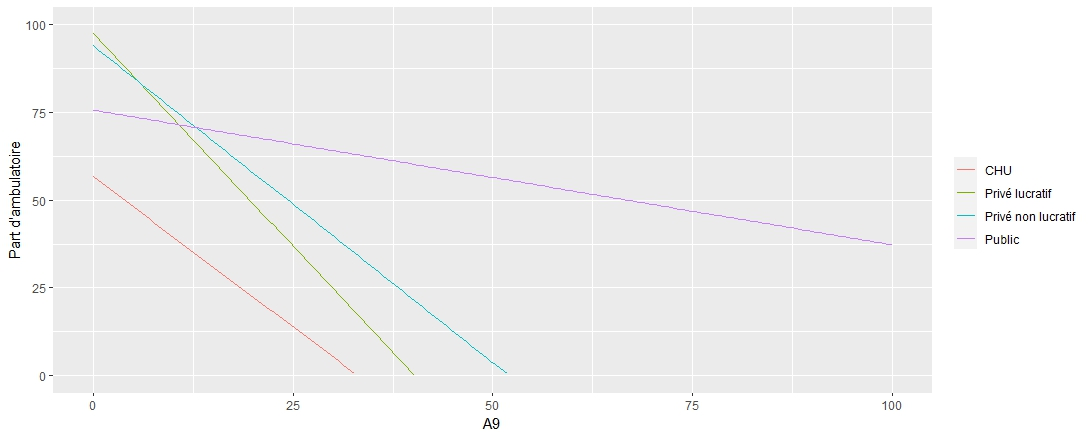
\includegraphics[scale=0.7]{Images/A9_inter_chir.jpeg}
    \label{inter_A9_chir}
\end{figure}

Points d'intersection (A9, Part d'ambulatoire):

\begin{itemize}
    \item Privé lucratif - Privé non lucratif : $(5.708923,83.69767)$
    \item Privé lucratif - Public : $(10.71357,71.55917)$
    \item Privé non lucratif - Public : $(12.89366,70.72169)$
\end{itemize}


\begin{table}[!htbp] \centering 
  \caption{Estimation des coefficients du modèle \ref{eqn:controle_inter}} 
  \label{controle_inter2} 
\begin{tabular}{@{\extracolsep{5pt}}lD{.}{.}{-3} D{.}{.}{-3} D{.}{.}{-3} } 
\\[-1.8ex]\hline 
\hline \\[-1.8ex] 
 & \multicolumn{3}{c}{\textit{Dependent variable:}} \\ 
\cline{2-4} 
\\[-1.8ex] & \multicolumn{3}{c}{Pourcentage d'ambulatoire} \\ 
 & \multicolumn{1}{c}{default} & \multicolumn{1}{c}{robust} & \multicolumn{1}{c}{robust and clustered} \\ 
\\[-1.8ex] & \multicolumn{1}{c}{(1)} & \multicolumn{1}{c}{(2)} & \multicolumn{1}{c}{(3)}\\ 
\hline \\[-1.8ex] 
 Privé lucratif & 40.840^{***} & 40.840^{***} & 40.840^{***} \\ 
  & (1.188) & (0.950) & (1.656) \\ 
  Privé non lucratif & 37.304^{***} & 37.304^{***} & 37.304^{***} \\ 
  & (1.224) & (1.008) & (1.768) \\ 
  Public & 18.970^{***} & 18.970^{***} & 18.970^{***} \\ 
  & (1.245) & (1.025) & (1.799) \\ 
  A9 & -1.714^{***} & -1.714^{***} & -1.714^{***} \\ 
  & (0.100) & (0.080) & (0.140) \\ 
  tarification & -0.121^{***} & -0.121^{***} & -0.121^{***} \\ 
  & (0.0005) & (0.001) & (0.001) \\ 
  A10 & -0.427 & -0.427 & -0.427 \\ 
  & (0.317) & (0.281) & (0.507) \\ 
  A11 & -0.683^{***} & -0.683^{***} & -0.683^{***} \\ 
  & (0.103) & (0.120) & (0.198) \\ 
  Privé lucratif*A9 & -2.425^{***} & -2.425^{***} & -2.425^{***} \\ 
  & (0.103) & (0.087) & (0.151) \\ 
  Privé non lucratif*A9 & -1.806^{***} & -1.806^{***} & -1.806^{***} \\ 
  & (0.106) & (0.088) & (0.155) \\ 
  Public*A9 & -0.384^{***} & -0.384^{***} & -0.384^{***} \\ 
  & (0.104) & (0.085) & (0.149) \\ 
  A9*tarification & 0.007^{***} & 0.007^{***} & 0.007^{***} \\ 
  & (0.0001) & (0.00005) & (0.0001) \\ 
  A10*A11 & 0.242 & 0.242 & 0.242 \\ 
  & (0.245) & (0.219) & (0.387) \\ 
  Constant & 56.705^{***} & 56.705^{***} & 56.705^{***} \\ 
  & (1.190) & (0.952) & (1.662) \\ 
 \hline \\[-1.8ex] 
Observations & \multicolumn{1}{c}{617,531} & \multicolumn{1}{c}{617,531} & \multicolumn{1}{c}{617,531} \\ 
R$^{2}$ & \multicolumn{1}{c}{0.247} & \multicolumn{1}{c}{0.247} & \multicolumn{1}{c}{0.247} \\ 
Adjusted R$^{2}$ & \multicolumn{1}{c}{0.247} & \multicolumn{1}{c}{0.247} & \multicolumn{1}{c}{0.247} \\ 
Residual Std. Error (df = 617518) & \multicolumn{1}{c}{281.366} & \multicolumn{1}{c}{281.366} & \multicolumn{1}{c}{281.366} \\ 
F Statistic (df = 12; 617518) & \multicolumn{1}{c}{16,910.920$^{***}$} & \multicolumn{1}{c}{16,910.920$^{***}$} & \multicolumn{1}{c}{16,910.920$^{***}$} \\ 
\hline 
\hline \\[-1.8ex] 
\textit{Note:}  & \multicolumn{3}{r}{$^{*}$p$<$0.1; $^{**}$p$<$0.05; $^{***}$p$<$0.01} \\ 
\end{tabular} 
\end{table} 


\clearpage
\subsection{Exérèse des amygdales et végétations}

Nous allons ici étudier une sous-catégorie d'actes chirurgicaux, les exérèses d'amygdales qui sont des actes programmables et effectués de nombreuses fois, en effet, chaque acte CCAM est a été effectué plus de 5000 fois sur l'ensemble des années étudiées. De plus, pour chacun de ces actes, le pourcentage moyen d'ambulatoire est compris entre 50 et 70\%. Parmi ces actes, on compte notamment les \textit{adénoïdectomies}, les \textit{amygdalectomies} et les \textit{exérèses de moignon amygdalien}.\\

\begin{table}[ht]
\centering
\caption{Pourcentage moyen d'actes effectués en ambulatoire (\%)} 
\label{part_ambu_tabu_amy}
\begin{tabular}{r|cccc|c}
  \hline
 & CHU & Privé lucratif & Privé non lucratif & Public & Total \\ 
  \hline
2015 & 45.63 & 67.68 & 62.70 & 54.64 & 62.99 \\ 
  2016 & 47.50 & 67.60 & 64.31 & 54.98 & 62.99 \\ 
  2017 & 47.98 & 68.21 & 66.21 & 54.81 & 63.38 \\ 
  2018 & 49.48 & 68.25 & 68.91 & 53.78 & 63.50 \\ 
  2019 & 49.64 & 69.98 & 71.31 & 56.60 & 65.34 \\ 
  \hline
  Total & 48.09 & 68.29 & 66.70 & 54.95 & 63.61 \\ 
   \hline
\end{tabular}

\bigskip

\begin{tabular}{ccccc}
  \hline
Min. & 1er Qu. & Médiane & 3e Qu. & Max. \\ 
  \hline
0.00 & 0.00 & 91.98 & 99.79 & 100.00  \\ 
   \hline
\end{tabular}
\end{table}


\begin{table}[!ht]
\centering
\caption{Durée moyenne des séjours} 
\label{dms_tabu_amy}
\begin{tabular}{r|cccc|c}
  \hline
 & CHU & Privé lucratif & Privé non lucratif & Public & Total \\ 
  \hline
2015 & 1.15 & 0.42 & 0.51 & 0.67 & 0.53 \\ 
  2016 & 1.08 & 0.41 & 0.48 & 0.63 & 0.52 \\ 
  2017 & 1.02 & 0.39 & 0.45 & 0.63 & 0.51 \\ 
  2018 & 1.04 & 0.37 & 0.41 & 0.65 & 0.50 \\ 
  2019 & 1.00 & 0.34 & 0.37 & 0.60 & 0.46 \\
  \hline
  Total & 1.06 & 0.39 & 0.44 & 0.64 & 0.51 \\ 
   \hline
\end{tabular}

\bigskip

\begin{tabular}{ccccc}
  \hline
Min. & 1er Qu. & Médiane & 3e Qu. & Max. \\ 
  \hline
0.00 & 0.00 & 0.10 & 0.99 & 13.68 \\ 
   \hline
\end{tabular}
\end{table}

Les tableaux \ref{part_ambu_tabu_amy} et \ref{dms_tabu_amy} présentent les moyennes issues des modèles linéaires de base. On observe que la distribution est assez irrégulière puisque que la médiane est située à 92\% pour la part d'ambulatoire.\\

Le tableau \ref{part_ambu_select_amy} présente les estimations des coefficients des modèles \ref{eqn:cat}, \ref{eqn:annee} et \ref{eqn:equation_base}. On constate également que les écarts entre les catégories d'établissements sont plus marqués que pour l'étude des actes chirurgicaux sélectionnés.

\begin{table}[!htbp] \centering 
  \caption{Modèles de base appliqué à la part d’actes en ambulatoire} 
  \label{part_ambu_select_amy} 
\begin{tabular}{@{\extracolsep{5pt}}lD{.}{.}{-3} D{.}{.}{-3} D{.}{.}{-3} } 
\\[-1.8ex]\hline 
\hline \\[-1.8ex] 
 & \multicolumn{3}{c}{\textit{Dependent variable:}} \\ 
\cline{2-4} 
\\[-1.8ex] & \multicolumn{3}{c}{Pourcentage d'ambulatoire} \\ 
 & \multicolumn{1}{c}{default} & \multicolumn{1}{c}{robust} & \multicolumn{1}{c}{robust and clustered} \\ 
\\[-1.8ex] & \multicolumn{1}{c}{(1)} & \multicolumn{1}{c}{(2)} & \multicolumn{1}{c}{(3)}\\ 
\hline \\[-1.8ex] 
 Privé lucratif & 20.204^{***} & 20.204^{***} & 20.204^{***} \\ 
  & (1.338) & (1.445) & (2.898) \\ 
  Privé non lucratif & 18.604^{***} & 18.604^{***} & 18.604^{***} \\ 
  & (1.839) & (2.024) & (4.048) \\ 
  Public & 6.859^{***} & 6.859^{***} & 6.859^{**} \\ 
  & (1.523) & (1.571) & (3.140) \\ 
  Constant & 48.091^{***} & 48.091^{***} & 48.091^{***} \\ 
  & (1.245) & (1.336) & (2.678) \\ 
 \hline \\[-1.8ex] 
Observations & \multicolumn{1}{c}{11,748} & \multicolumn{1}{c}{11,748} & \multicolumn{1}{c}{11,748} \\ 
R$^{2}$ & \multicolumn{1}{c}{0.029} & \multicolumn{1}{c}{0.029} & \multicolumn{1}{c}{0.029} \\ 
Adjusted R$^{2}$ & \multicolumn{1}{c}{0.029} & \multicolumn{1}{c}{0.029} & \multicolumn{1}{c}{0.029} \\ 
Residual Std. Error (df = 11744) & \multicolumn{1}{c}{289.179} & \multicolumn{1}{c}{289.179} & \multicolumn{1}{c}{289.179} \\ 
F Statistic (df = 3; 11744) & \multicolumn{1}{c}{116.623$^{***}$} & \multicolumn{1}{c}{116.623$^{***}$} & \multicolumn{1}{c}{116.623$^{***}$} \\ 
\hline 
\hline \\[-1.8ex] 
\end{tabular} 

\bigskip


\begin{tabular}{@{\extracolsep{5pt}}lD{.}{.}{-3} D{.}{.}{-3} D{.}{.}{-3} } 
\\[-1.8ex]\hline 
\hline \\[-1.8ex] 
 & \multicolumn{3}{c}{\textit{Dependent variable:}} \\ 
\cline{2-4} 
\\[-1.8ex] & \multicolumn{3}{c}{Pourcentage d'ambulatoire} \\ 
 & \multicolumn{1}{c}{default} & \multicolumn{1}{c}{robust} & \multicolumn{1}{c}{robust and clustered} \\ 
\\[-1.8ex] & \multicolumn{1}{c}{(1)} & \multicolumn{1}{c}{(2)} & \multicolumn{1}{c}{(3)}\\ 
\hline \\[-1.8ex] 
 2016 & 0.004 & 0.004 & 0.004 \\ 
  & (1.209) & (1.316) & (0.572) \\ 
  2017 & 0.395 & 0.395 & 0.395 \\ 
  & (1.224) & (1.320) & (0.641) \\ 
  2018 & 0.513 & 0.513 & 0.513 \\ 
  & (1.242) & (1.326) & (0.701) \\ 
  2019 & 2.355^{*} & 2.355^{*} & 2.355^{***} \\ 
  & (1.245) & (1.316) & (0.763) \\ 
  Constant & 62.986^{***} & 62.986^{***} & 62.986^{***} \\ 
  & (0.853) & (0.923) & (0.923) \\ 
 \hline \\[-1.8ex] 
Observations & \multicolumn{1}{c}{11,748} & \multicolumn{1}{c}{11,748} & \multicolumn{1}{c}{11,748} \\ 
R$^{2}$ & \multicolumn{1}{c}{0.0004} & \multicolumn{1}{c}{0.0004} & \multicolumn{1}{c}{0.0004} \\ 
Adjusted R$^{2}$ & \multicolumn{1}{c}{0.0001} & \multicolumn{1}{c}{0.0001} & \multicolumn{1}{c}{0.0001} \\ 
Residual Std. Error (df = 11743) & \multicolumn{1}{c}{293.407} & \multicolumn{1}{c}{293.407} & \multicolumn{1}{c}{293.407} \\ 
F Statistic (df = 4; 11743) & \multicolumn{1}{c}{1.197} & \multicolumn{1}{c}{1.197} & \multicolumn{1}{c}{1.197} \\ 
\hline 
\hline \\[-1.8ex] 
\textit{Note:}  & \multicolumn{3}{r}{$^{*}$p$<$0.1; $^{**}$p$<$0.05; $^{***}$p$<$0.01} \\ 
\end{tabular} 
\end{table}

\begin{table}[!htbp] \centering 
\scalebox{0.85}{
\begin{tabular}{@{\extracolsep{5pt}}lD{.}{.}{-3} D{.}{.}{-3} D{.}{.}{-3} } 
\\[-1.8ex]\hline 
\hline \\[-1.8ex] 
 & \multicolumn{3}{c}{\textit{Dependent variable:}} \\ 
\cline{2-4} 
\\[-1.8ex] & \multicolumn{3}{c}{Pourcentage d'ambulatoire} \\ 
 & \multicolumn{1}{c}{default} & \multicolumn{1}{c}{robust} & \multicolumn{1}{c}{robust and clustered} \\ 
\\[-1.8ex] & \multicolumn{1}{c}{(1)} & \multicolumn{1}{c}{(2)} & \multicolumn{1}{c}{(3)}\\ 
\hline \\[-1.8ex] 
 Privé lucratif & 22.043^{***} & 22.043^{***} & 22.043^{***} \\ 
  & (3.080) & (3.221) & (3.221) \\ 
  Privé non lucratif & 17.065^{***} & 17.065^{***} & 17.065^{***} \\ 
  & (4.201) & (4.588) & (4.589) \\ 
  Public & 9.010^{***} & 9.010^{**} & 9.010^{**} \\ 
  & (3.488) & (3.504) & (3.504) \\ 
  2016 & 1.865 & 1.865 & 1.865 \\ 
  & (4.016) & (4.275) & (2.131) \\ 
  2017 & 2.342 & 2.342 & 2.342 \\ 
  & (3.983) & (4.212) & (2.158) \\ 
  2018 & 3.844 & 3.844 & 3.844^{*} \\ 
  & (4.011) & (4.204) & (2.333) \\ 
  2019 & 4.006 & 4.006 & 4.006 \\ 
  & (3.995) & (4.212) & (2.464) \\ 
  Privé lucratif*2016 & -1.945 & -1.945 & -1.945 \\ 
  & (4.283) & (4.606) & (2.251) \\ 
  Privé non lucratif*2016 & -0.249 & -0.249 & -0.249 \\ 
  & (5.875) & (6.536) & (3.129) \\ 
  Public*2016 & -1.527 & -1.527 & -1.527 \\ 
  & (4.846) & (4.986) & (2.406) \\ 
  Privé lucratif*2017 & -1.809 & -1.809 & -1.809 \\ 
  & (4.261) & (4.548) & (2.299) \\ 
  Privé non lucratif*2017 & 1.174 & 1.174 & 1.174 \\ 
  & (5.848) & (6.449) & (3.216) \\ 
  Public*2017 & -2.171 & -2.171 & -2.171 \\ 
  & (4.841) & (4.949) & (2.552) \\ 
  Privé lucratif*2018 & -3.269 & -3.269 & -3.269 \\ 
  & (4.297) & (4.546) & (2.495) \\ 
  Privé non lucratif*2018 & 2.367 & 2.367 & 2.367 \\ 
  & (5.884) & (6.384) & (3.506) \\ 
  Public*2018 & -4.707 & -4.707 & -4.707^{*} \\ 
  & (4.882) & (4.951) & (2.748) \\ 
  Privé lucratif*2019 & -1.697 & -1.697 & -1.697 \\ 
  & (4.284) & (4.543) & (2.652) \\ 
  Privé non lucratif*2019 & 4.604 & 4.604 & 4.604 \\ 
  & (5.857) & (6.340) & (3.854) \\ 
  Public*2019 & -2.047 & -2.047 & -2.047 \\ 
  & (4.881) & (4.959) & (2.897) \\ 
  Constant & 45.633^{***} & 45.633^{***} & 45.633^{***} \\ 
  & (2.898) & (2.991) & (2.992) \\ 
 \hline \\[-1.8ex] 
Observations & \multicolumn{1}{c}{11,748} & \multicolumn{1}{c}{11,748} & \multicolumn{1}{c}{11,748} \\ 
R$^{2}$ & \multicolumn{1}{c}{0.030} & \multicolumn{1}{c}{0.030} & \multicolumn{1}{c}{0.030} \\ 
Adjusted R$^{2}$ & \multicolumn{1}{c}{0.028} & \multicolumn{1}{c}{0.028} & \multicolumn{1}{c}{0.028} \\ 
Residual Std. Error (df = 11728) & \multicolumn{1}{c}{289.245} & \multicolumn{1}{c}{289.245} & \multicolumn{1}{c}{289.245} \\ 
F Statistic (df = 19; 11728) & \multicolumn{1}{c}{18.963$^{***}$} & \multicolumn{1}{c}{18.963$^{***}$} & \multicolumn{1}{c}{18.963$^{***}$} \\ 
\hline 
\hline \\[-1.8ex]  
\end{tabular} 
}
\end{table}

\clearpage

On ajoute la variable de contrôle, \textit{A9}, voir tableaux \ref{reg_amy_A9}. Dans le cas hypothétique où $A9 = 0$, on constate que, pour chaque catégorie d'établissement, la part moyenne d'actes effectués en ambulatoire augmente. Les écarts entre les différentes catégories d'établissements ont bien diminué et tous les hôpitaux privés sont au même niveau. Comme attendu la variable \textit{A9} a bien un coefficient négatif.\\

\begin{table}[!htbp] \centering 
  \caption{Modèles de base avec contrôle par A9} 
  \label{reg_amy_A9} 
\begin{tabular}{@{\extracolsep{5pt}}lD{.}{.}{-3} D{.}{.}{-3} D{.}{.}{-3} } 
\\[-1.8ex]\hline 
\hline \\[-1.8ex] 
 & \multicolumn{3}{c}{\textit{Dependent variable:}} \\ 
\cline{2-4} 
\\[-1.8ex] & \multicolumn{3}{c}{Pourcentage d'ambulatoire} \\ 
 & \multicolumn{1}{c}{default} & \multicolumn{1}{c}{robust} & \multicolumn{1}{c}{robust and clustered} \\ 
\\[-1.8ex] & \multicolumn{1}{c}{(1)} & \multicolumn{1}{c}{(2)} & \multicolumn{1}{c}{(3)}\\ 
\hline \\[-1.8ex] 
 Privé lucratif & 14.665^{***} & 14.665^{***} & 14.665^{***} \\ 
  & (2.028) & (2.074) & (4.018) \\ 
  Privé non lucratif & 14.780^{***} & 14.780^{***} & 14.780^{***} \\ 
  & (2.119) & (2.247) & (4.432) \\ 
  Public & 7.755^{***} & 7.755^{***} & 7.755^{**} \\ 
  & (1.542) & (1.597) & (3.190) \\ 
  A9 & -0.648^{***} & -0.648^{***} & -0.648^{*} \\ 
  & (0.178) & (0.178) & (0.334) \\ 
  Constant & 55.417^{***} & 55.417^{***} & 55.417^{***} \\ 
  & (2.370) & (2.411) & (4.614) \\ 
 \hline \\[-1.8ex] 
Observations & \multicolumn{1}{c}{11,748} & \multicolumn{1}{c}{11,748} & \multicolumn{1}{c}{11,748} \\ 
R$^{2}$ & \multicolumn{1}{c}{0.030} & \multicolumn{1}{c}{0.030} & \multicolumn{1}{c}{0.030} \\ 
Adjusted R$^{2}$ & \multicolumn{1}{c}{0.030} & \multicolumn{1}{c}{0.030} & \multicolumn{1}{c}{0.030} \\ 
Residual Std. Error (df = 11743) & \multicolumn{1}{c}{289.029} & \multicolumn{1}{c}{289.029} & \multicolumn{1}{c}{289.029} \\ 
F Statistic (df = 4; 11743) & \multicolumn{1}{c}{90.856$^{***}$} & \multicolumn{1}{c}{90.856$^{***}$} & \multicolumn{1}{c}{90.856$^{***}$} \\ 
\hline 
\hline \\[-1.8ex] 
\textit{Note:}  & \multicolumn{3}{r}{$^{*}$p$<$0.1; $^{**}$p$<$0.05; $^{***}$p$<$0.01} \\ 
\end{tabular} 
\end{table} 

\begin{table}[!htbp] \centering  
\begin{tabular}{@{\extracolsep{5pt}}lD{.}{.}{-3} D{.}{.}{-3} D{.}{.}{-3} } 
\\[-1.8ex]\hline 
\hline \\[-1.8ex] 
 & \multicolumn{3}{c}{\textit{Dependent variable:}} \\ 
\cline{2-4} 
\\[-1.8ex] & \multicolumn{3}{c}{Pourcentage d'ambulatoire} \\ 
 & \multicolumn{1}{c}{default} & \multicolumn{1}{c}{robust} & \multicolumn{1}{c}{robust and clustered} \\ 
\\[-1.8ex] & \multicolumn{1}{c}{(1)} & \multicolumn{1}{c}{(2)} & \multicolumn{1}{c}{(3)}\\ 
\hline \\[-1.8ex] 
 2016 & 0.363 & 0.363 & 0.363 \\ 
  & (1.194) & (1.312) & (0.571) \\ 
  2017 & 1.061 & 1.061 & 1.061^{*} \\ 
  & (1.210) & (1.314) & (0.642) \\ 
  2018 & 1.407 & 1.407 & 1.407^{**} \\ 
  & (1.227) & (1.320) & (0.705) \\ 
  2019 & 3.239^{***} & 3.239^{**} & 3.239^{***} \\ 
  & (1.231) & (1.310) & (0.764) \\ 
  A9 & -1.418^{***} & -1.418^{***} & -1.418^{***} \\ 
  & (0.082) & (0.083) & (0.163) \\ 
  Constant & 70.584^{***} & 70.584^{***} & 70.584^{***} \\ 
  & (0.949) & (1.049) & (1.371) \\ 
 \hline \\[-1.8ex] 
Observations & \multicolumn{1}{c}{11,748} & \multicolumn{1}{c}{11,748} & \multicolumn{1}{c}{11,748} \\ 
R$^{2}$ & \multicolumn{1}{c}{0.026} & \multicolumn{1}{c}{0.026} & \multicolumn{1}{c}{0.026} \\ 
Adjusted R$^{2}$ & \multicolumn{1}{c}{0.025} & \multicolumn{1}{c}{0.025} & \multicolumn{1}{c}{0.025} \\ 
Residual Std. Error (df = 11742) & \multicolumn{1}{c}{289.709} & \multicolumn{1}{c}{289.709} & \multicolumn{1}{c}{289.709} \\ 
F Statistic (df = 5; 11742) & \multicolumn{1}{c}{61.527$^{***}$} & \multicolumn{1}{c}{61.527$^{***}$} & \multicolumn{1}{c}{61.527$^{***}$} \\ 
\hline 
\hline \\[-1.8ex] 
\textit{Note:}  & \multicolumn{3}{r}{$^{*}$p$<$0.1; $^{**}$p$<$0.05; $^{***}$p$<$0.01} \\ 
\end{tabular} 
\end{table}

\begin{table}[!htbp] \centering 
\scalebox{0.85}{
\begin{tabular}{@{\extracolsep{5pt}}lD{.}{.}{-3} D{.}{.}{-3} D{.}{.}{-3} } 
\\[-1.8ex]\hline 
\hline \\[-1.8ex] 
 & \multicolumn{3}{c}{\textit{Dependent variable:}} \\ 
\cline{2-4} 
\\[-1.8ex] & \multicolumn{3}{c}{Pourcentage d'ambulatoire} \\ 
 & \multicolumn{1}{c}{default} & \multicolumn{1}{c}{robust} & \multicolumn{1}{c}{robust and clustered} \\ 
\\[-1.8ex] & \multicolumn{1}{c}{(1)} & \multicolumn{1}{c}{(2)} & \multicolumn{1}{c}{(3)}\\ 
\hline \\[-1.8ex] 
 Privé lucratif & 16.494^{***} & 16.494^{***} & 16.494^{***} \\ 
  & (3.417) & (3.529) & (4.203) \\ 
  Privé non lucratif & 13.343^{***} & 13.343^{***} & 13.343^{***} \\ 
  & (4.315) & (4.676) & (4.906) \\ 
  Public & 9.643^{***} & 9.643^{***} & 9.643^{***} \\ 
  & (3.490) & (3.511) & (3.537) \\ 
  2016 & 1.915 & 1.915 & 1.915 \\ 
  & (4.014) & (4.276) & (2.130) \\ 
  2017 & 2.536 & 2.536 & 2.536 \\ 
  & (3.981) & (4.212) & (2.161) \\ 
  2018 & 4.272 & 4.272 & 4.272^{*} \\ 
  & (4.010) & (4.206) & (2.350) \\ 
  2019 & 4.411 & 4.411 & 4.411^{*} \\ 
  & (3.994) & (4.214) & (2.478) \\ 
  A9 & -0.672^{***} & -0.672^{***} & -0.672^{**} \\ 
  & (0.180) & (0.179) & (0.338) \\ 
  Privé lucratif*2016 & -1.974 & -1.974 & -1.974 \\ 
  & (4.280) & (4.607) & (2.250) \\ 
  Privé non lucratif*2016 & -0.424 & -0.424 & -0.424 \\ 
  & (5.872) & (6.533) & (3.128) \\ 
  Public*2016 & -1.299 & -1.299 & -1.299 \\ 
  & (4.844) & (4.987) & (2.406) \\ 
  Privé lucratif*2017 & -1.961 & -1.961 & -1.961 \\ 
  & (4.259) & (4.549) & (2.301) \\ 
  Privé non lucratif*2017 & 0.928 & 0.928 & 0.928 \\ 
  & (5.845) & (6.446) & (3.216) \\ 
  Public*2017 & -1.742 & -1.742 & -1.742 \\ 
  & (4.840) & (4.950) & (2.556) \\ 
  Privé lucratif*2018 & -3.644 & -3.644 & -3.644 \\ 
  & (4.296) & (4.548) & (2.509) \\ 
  Privé non lucratif*2018 & 1.938 & 1.938 & 1.938 \\ 
  & (5.882) & (6.383) & (3.515) \\ 
  Public*2018 & -4.320 & -4.320 & -4.320 \\ 
  & (4.880) & (4.952) & (2.755) \\ 
  Privé lucratif*2019 & -2.088 & -2.088 & -2.088 \\ 
  & (4.283) & (4.545) & (2.663) \\ 
  Privé non lucratif*2019 & 4.259 & 4.259 & 4.259 \\ 
  & (5.854) & (6.339) & (3.855) \\ 
  Public*2019 & -1.525 & -1.525 & -1.525 \\ 
  & (4.880) & (4.960) & (2.902) \\ 
  Constant & 53.012^{***} & 53.012^{***} & 53.012^{***} \\ 
  & (3.504) & (3.573) & (4.734) \\ 
 \hline \\[-1.8ex] 
Observations & \multicolumn{1}{c}{11,748} & \multicolumn{1}{c}{11,748} & \multicolumn{1}{c}{11,748} \\ 
R$^{2}$ & \multicolumn{1}{c}{0.031} & \multicolumn{1}{c}{0.031} & \multicolumn{1}{c}{0.031} \\ 
Adjusted R$^{2}$ & \multicolumn{1}{c}{0.029} & \multicolumn{1}{c}{0.029} & \multicolumn{1}{c}{0.029} \\ 
Residual Std. Error (df = 11727) & \multicolumn{1}{c}{289.085} & \multicolumn{1}{c}{289.085} & \multicolumn{1}{c}{289.085} \\ 
F Statistic (df = 20; 11727) & \multicolumn{1}{c}{18.735$^{***}$} & \multicolumn{1}{c}{18.735$^{***}$} & \multicolumn{1}{c}{18.735$^{***}$} \\ 
\hline 
\hline \\[-1.8ex]  
\end{tabular} 
}
\end{table} 

\clearpage


On rajoute la tarification comme variable de contrôle, voit tableau \ref{reg_A9_tarif_amy}. La valeur de la constante est aberrante, cela est dû au fait que la variable de tarification est agrégé au niveau de l'acte CCAM et qu'on utilise dans cette partie seulement une quinzaine d'actes différents, la tarification ne peut donc prendre que 15 valeurs différentes. On ne va donc plus utiliser cette variable dans la suite.\\

\begin{table}[!htbp] \centering 
  \caption{Modèles de base avec contrôle par A9 et tarification} 
  \label{reg_A9_tarif_amy} 
\begin{tabular}{@{\extracolsep{5pt}}lD{.}{.}{-3} D{.}{.}{-3} D{.}{.}{-3} } 
\\[-1.8ex]\hline 
\hline \\[-1.8ex] 
 & \multicolumn{3}{c}{\textit{Dependent variable:}} \\ 
\cline{2-4} 
\\[-1.8ex] & \multicolumn{3}{c}{Pourcentage d'ambulatoire} \\ 
 & \multicolumn{1}{c}{default} & \multicolumn{1}{c}{robust} & \multicolumn{1}{c}{robust and clustered} \\ 
\\[-1.8ex] & \multicolumn{1}{c}{(1)} & \multicolumn{1}{c}{(2)} & \multicolumn{1}{c}{(3)}\\ 
\hline \\[-1.8ex] 
 Privé lucratif & 15.945^{***} & 15.945^{***} & 15.945^{***} \\ 
  & (1.784) & (1.831) & (3.497) \\ 
  Privé non lucratif & 15.970^{***} & 15.970^{***} & 15.970^{***} \\ 
  & (1.864) & (1.949) & (3.775) \\ 
  Public & 6.530^{***} & 6.530^{***} & 6.530^{**} \\ 
  & (1.356) & (1.401) & (2.750) \\ 
  A9 & -0.439^{***} & -0.439^{***} & -0.439 \\ 
  & (0.157) & (0.154) & (0.288) \\ 
  tarification & -1.064^{***} & -1.064^{***} & -1.064^{***} \\ 
  & (0.018) & (0.012) & (0.022) \\ 
  Constant & 141.495^{***} & 141.495^{***} & 141.495^{***} \\ 
  & (2.551) & (2.349) & (4.380) \\ 
 \hline \\[-1.8ex] 
Observations & \multicolumn{1}{c}{11,748} & \multicolumn{1}{c}{11,748} & \multicolumn{1}{c}{11,748} \\ 
R$^{2}$ & \multicolumn{1}{c}{0.249} & \multicolumn{1}{c}{0.249} & \multicolumn{1}{c}{0.249} \\ 
Adjusted R$^{2}$ & \multicolumn{1}{c}{0.249} & \multicolumn{1}{c}{0.249} & \multicolumn{1}{c}{0.249} \\ 
Residual Std. Error (df = 11742) & \multicolumn{1}{c}{254.281} & \multicolumn{1}{c}{254.281} & \multicolumn{1}{c}{254.281} \\ 
F Statistic (df = 5; 11742) & \multicolumn{1}{c}{779.839$^{***}$} & \multicolumn{1}{c}{779.839$^{***}$} & \multicolumn{1}{c}{779.839$^{***}$} \\ 
\hline 
\hline \\[-1.8ex] 
\textit{Note:}  & \multicolumn{3}{r}{$^{*}$p$<$0.1; $^{**}$p$<$0.05; $^{***}$p$<$0.01} \\ 
\end{tabular} 
\end{table} 
\clearpage

Le tableaux \ref{reg_controle_A1_amy} présente les résultats obtenus pour le modèle \ref{eqn:cat} contrôlé par \textit{A9}, \textit{A10} et \textit{A11}. L'ajout des deux dernière variables permet de diminuer l'écart entre les catégories d'établissement mais il augmente grandement les écarts-types au point que la différence entre CHU et autres hôpitaux publics n'est plus significative malgré un coefficient estimé à 4. Cette perte majeure de significativité est sûrement due à la sélection des actes de la sous-catégorie et au fait que \textit{A10} et \textit{A11} contiennent de nombreuses valeurs nulles (ces variables de contrôle ne sont pas significatives non-plus).\\

\begin{table}[!htbp] \centering 
  \caption{Modèle de base avec contrôle par A9, A10 et A11} 
  \label{reg_controle_A1_amy} 
\begin{tabular}{@{\extracolsep{5pt}}lD{.}{.}{-3} D{.}{.}{-3} D{.}{.}{-3} } 
\\[-1.8ex]\hline 
\hline \\[-1.8ex] 
 & \multicolumn{3}{c}{\textit{Dependent variable:}} \\ 
\cline{2-4} 
\\[-1.8ex] & \multicolumn{3}{c}{Pourcentage d'ambulatoire} \\ 
 & \multicolumn{1}{c}{default} & \multicolumn{1}{c}{robust} & \multicolumn{1}{c}{robust and clustered} \\ 
\\[-1.8ex] & \multicolumn{1}{c}{(1)} & \multicolumn{1}{c}{(2)} & \multicolumn{1}{c}{(3)}\\ 
\hline \\[-1.8ex] 
 Privé lucratif & 10.470^{***} & 10.470^{***} & 10.470 \\ 
  & (3.599) & (3.666) & (6.845) \\ 
  Privé non lucratif & 10.797^{***} & 10.797^{***} & 10.797 \\ 
  & (3.570) & (3.660) & (6.937) \\ 
  Public & 3.841 & 3.841 & 3.841 \\ 
  & (3.157) & (3.218) & (6.063) \\ 
  A9 & -0.649^{***} & -0.649^{***} & -0.649^{*} \\ 
  & (0.179) & (0.178) & (0.334) \\ 
  A10 & -2.458 & -2.458 & -2.458 \\ 
  & (2.259) & (2.211) & (4.132) \\ 
  A11 & -1.060 & -1.060 & -1.060 \\ 
  & (1.339) & (1.391) & (2.289) \\ 
  Constant & 59.640^{***} & 59.640^{***} & 59.640^{***} \\ 
  & (3.815) & (3.884) & (7.237) \\ 
 \hline \\[-1.8ex] 
Observations & \multicolumn{1}{c}{11,748} & \multicolumn{1}{c}{11,748} & \multicolumn{1}{c}{11,748} \\ 
R$^{2}$ & \multicolumn{1}{c}{0.030} & \multicolumn{1}{c}{0.030} & \multicolumn{1}{c}{0.030} \\ 
Adjusted R$^{2}$ & \multicolumn{1}{c}{0.030} & \multicolumn{1}{c}{0.030} & \multicolumn{1}{c}{0.030} \\ 
Residual Std. Error (df = 11741) & \multicolumn{1}{c}{289.027} & \multicolumn{1}{c}{289.027} & \multicolumn{1}{c}{289.027} \\ 
F Statistic (df = 6; 11741) & \multicolumn{1}{c}{60.926$^{***}$} & \multicolumn{1}{c}{60.926$^{***}$} & \multicolumn{1}{c}{60.926$^{***}$} \\ 
\hline 
\hline \\[-1.8ex] 
\textit{Note:}  & \multicolumn{3}{r}{$^{*}$p$<$0.1; $^{**}$p$<$0.05; $^{***}$p$<$0.01} \\ 
\end{tabular} 
\end{table}  

\clearpage

L'ajout du terme d'interaction entre \textit{A10} et \textit{A11} ne corrige que faiblement les estimations et augmente une fois de plus les écarts-types (voir tableaux \ref{reg_controle_inter_A1_amy}).\\

\begin{table}[!htbp] \centering 
  \caption{Modèle de base avec contrôle par A9, A10 et A11 (+interaction entre A10 et A11)} 
  \label{reg_controle_inter_A1_amy} 
\begin{tabular}{@{\extracolsep{5pt}}lD{.}{.}{-3} D{.}{.}{-3} D{.}{.}{-3} } 
\\[-1.8ex]\hline 
\hline \\[-1.8ex] 
 & \multicolumn{3}{c}{\textit{Dependent variable:}} \\ 
\cline{2-4} 
\\[-1.8ex] & \multicolumn{3}{c}{Pourcentage d'ambulatoire} \\ 
 & \multicolumn{1}{c}{default} & \multicolumn{1}{c}{robust} & \multicolumn{1}{c}{robust and clustered} \\ 
\\[-1.8ex] & \multicolumn{1}{c}{(1)} & \multicolumn{1}{c}{(2)} & \multicolumn{1}{c}{(3)}\\ 
\hline \\[-1.8ex] 
 Privé lucratif & 9.533^{***} & 9.533^{**} & 9.533 \\ 
  & (3.670) & (3.733) & (6.920) \\ 
  Privé non lucratif & 9.809^{***} & 9.809^{***} & 9.809 \\ 
  & (3.650) & (3.741) & (7.028) \\ 
  Public & 2.705 & 2.705 & 2.705 \\ 
  & (3.275) & (3.323) & (6.184) \\ 
  A9 & -0.652^{***} & -0.652^{***} & -0.652^{*} \\ 
  & (0.179) & (0.178) & (0.334) \\ 
  A10 & 1.129 & 1.129 & 1.129 \\ 
  & (3.565) & (3.541) & (6.884) \\ 
  A11 & -0.593 & -0.593 & -0.593 \\ 
  & (1.386) & (1.434) & (2.348) \\ 
  A10*A11 & -4.260 & -4.260 & -4.260 \\ 
  & (3.275) & (3.211) & (6.160) \\ 
  Constant & 60.574^{***} & 60.574^{***} & 60.574^{***} \\ 
  & (3.882) & (3.949) & (7.312) \\ 
 \hline \\[-1.8ex] 
Observations & \multicolumn{1}{c}{11,748} & \multicolumn{1}{c}{11,748} & \multicolumn{1}{c}{11,748} \\ 
R$^{2}$ & \multicolumn{1}{c}{0.030} & \multicolumn{1}{c}{0.030} & \multicolumn{1}{c}{0.030} \\ 
Adjusted R$^{2}$ & \multicolumn{1}{c}{0.030} & \multicolumn{1}{c}{0.030} & \multicolumn{1}{c}{0.030} \\ 
Residual Std. Error (df = 11740) & \multicolumn{1}{c}{289.019} & \multicolumn{1}{c}{289.019} & \multicolumn{1}{c}{289.019} \\ 
F Statistic (df = 7; 11740) & \multicolumn{1}{c}{52.467$^{***}$} & \multicolumn{1}{c}{52.467$^{***}$} & \multicolumn{1}{c}{52.467$^{***}$} \\ 
\hline 
\hline \\[-1.8ex] 
\textit{Note:}  & \multicolumn{3}{r}{$^{*}$p$<$0.1; $^{**}$p$<$0.05; $^{***}$p$<$0.01} \\ 
\end{tabular} 
\end{table} 

\begin{table}[!htbp] \centering 
\begin{tabular}{@{\extracolsep{5pt}}lD{.}{.}{-3} D{.}{.}{-3} D{.}{.}{-3} } 
\\[-1.8ex]\hline 
\hline \\[-1.8ex] 
 & \multicolumn{3}{c}{\textit{Dependent variable:}} \\ 
\cline{2-4} 
\\[-1.8ex] & \multicolumn{3}{c}{Pourcentage d'ambulatoire} \\ 
 & \multicolumn{1}{c}{default} & \multicolumn{1}{c}{robust} & \multicolumn{1}{c}{robust and clustered} \\ 
\\[-1.8ex] & \multicolumn{1}{c}{(1)} & \multicolumn{1}{c}{(2)} & \multicolumn{1}{c}{(3)}\\ 
\hline \\[-1.8ex] 
 2016 & 0.334 & 0.334 & 0.334 \\ 
  & (1.191) & (1.308) & (0.570) \\ 
  2017 & 1.214 & 1.214 & 1.214^{*} \\ 
  & (1.211) & (1.313) & (0.648) \\ 
  2018 & 1.507 & 1.507 & 1.507^{**} \\ 
  & (1.225) & (1.318) & (0.704) \\ 
  2019 & 3.394^{***} & 3.394^{***} & 3.394^{***} \\ 
  & (1.229) & (1.307) & (0.764) \\ 
  A9 & -1.177^{***} & -1.177^{***} & -1.177^{***} \\ 
  & (0.090) & (0.088) & (0.173) \\ 
  A10 & -1.933 & -1.933 & -1.933 \\ 
  & (3.393) & (3.361) & (6.542) \\ 
  A11 & -0.965 & -0.965 & -0.965 \\ 
  & (1.352) & (1.452) & (2.414) \\ 
  A10*A11 & -4.368 & -4.368 & -4.368 \\ 
  & (3.155) & (3.109) & (6.058) \\ 
  Constant & 70.150^{***} & 70.150^{***} & 70.150^{***} \\ 
  & (0.950) & (1.049) & (1.372) \\ 
 \hline \\[-1.8ex] 
Observations & \multicolumn{1}{c}{11,748} & \multicolumn{1}{c}{11,748} & \multicolumn{1}{c}{11,748} \\ 
R$^{2}$ & \multicolumn{1}{c}{0.030} & \multicolumn{1}{c}{0.030} & \multicolumn{1}{c}{0.030} \\ 
Adjusted R$^{2}$ & \multicolumn{1}{c}{0.029} & \multicolumn{1}{c}{0.029} & \multicolumn{1}{c}{0.029} \\ 
Residual Std. Error (df = 11739) & \multicolumn{1}{c}{289.100} & \multicolumn{1}{c}{289.100} & \multicolumn{1}{c}{289.100} \\ 
F Statistic (df = 8; 11739) & \multicolumn{1}{c}{45.186$^{***}$} & \multicolumn{1}{c}{45.186$^{***}$} & \multicolumn{1}{c}{45.186$^{***}$} \\ 
\hline 
\hline \\[-1.8ex] 
\textit{Note:}  & \multicolumn{3}{r}{$^{*}$p$<$0.1; $^{**}$p$<$0.05; $^{***}$p$<$0.01} \\ 
\end{tabular} 
\end{table}

\begin{table}[!htbp] \centering 
\scalebox{0.75}{
\begin{tabular}{@{\extracolsep{5pt}}lD{.}{.}{-3} D{.}{.}{-3} D{.}{.}{-3} } 
\\[-1.8ex]\hline 
\hline \\[-1.8ex] 
 & \multicolumn{3}{c}{\textit{Dependent variable:}} \\ 
\cline{2-4} 
\\[-1.8ex] & \multicolumn{3}{c}{Pourcentage d'ambulatoire} \\ 
 & \multicolumn{1}{c}{default} & \multicolumn{1}{c}{robust} & \multicolumn{1}{c}{robust and clustered} \\ 
\\[-1.8ex] & \multicolumn{1}{c}{(1)} & \multicolumn{1}{c}{(2)} & \multicolumn{1}{c}{(3)}\\ 
\hline \\[-1.8ex] 
 Privé lucratif & 10.755^{**} & 10.755^{**} & 10.755 \\ 
  & (4.579) & (4.643) & (7.030) \\ 
  Privé non lucratif & 7.738 & 7.738 & 7.738 \\ 
  & (5.249) & (5.524) & (7.378) \\ 
  Public & 4.033 & 4.033 & 4.033 \\ 
  & (4.533) & (4.515) & (6.372) \\ 
  2016 & 1.500 & 1.500 & 1.500 \\ 
  & (4.019) & (4.273) & (2.159) \\ 
  2017 & 2.688 & 2.688 & 2.688 \\ 
  & (3.982) & (4.211) & (2.166) \\ 
  2018 & 4.424 & 4.424 & 4.424^{*} \\ 
  & (4.013) & (4.209) & (2.372) \\ 
  2019 & 4.576 & 4.576 & 4.576^{*} \\ 
  & (3.998) & (4.217) & (2.495) \\ 
  A9 & -0.676^{***} & -0.676^{***} & -0.676^{**} \\ 
  & (0.180) & (0.179) & (0.338) \\ 
  A10 & 0.747 & 0.747 & 0.747 \\ 
  & (3.570) & (3.537) & (6.905) \\ 
  A11 & -1.022 & -1.022 & -1.022 \\ 
  & (1.403) & (1.439) & (2.390) \\ 
  Privé lucratif*2016 & -1.559 & -1.559 & -1.559 \\ 
  & (4.285) & (4.604) & (2.277) \\ 
  Privé non lucratif*2016 & -0.049 & -0.049 & -0.049 \\ 
  & (5.875) & (6.531) & (3.157) \\ 
  Public*2016 & -0.856 & -0.856 & -0.856 \\ 
  & (4.848) & (4.986) & (2.436) \\ 
  Privé lucratif*2017 & -2.023 & -2.023 & -2.023 \\ 
  & (4.262) & (4.548) & (2.309) \\ 
  Privé non lucratif*2017 & 0.883 & 0.883 & 0.883 \\ 
  & (5.847) & (6.441) & (3.218) \\ 
  Public*2017 & -1.832 & -1.832 & -1.832 \\ 
  & (4.841) & (4.949) & (2.560) \\ 
  Privé lucratif*2018 & -3.785 & -3.785 & -3.785 \\ 
  & (4.298) & (4.551) & (2.530) \\ 
  Privé non lucratif*2018 & 1.963 & 1.963 & 1.963 \\ 
  & (5.888) & (6.394) & (3.556) \\ 
  Public*2018 & -4.436 & -4.436 & -4.436 \\ 
  & (4.881) & (4.954) & (2.773) \\ 
  Privé lucratif*2019 & -2.235 & -2.235 & -2.235 \\ 
  & (4.287) & (4.549) & (2.679) \\ 
  Privé non lucratif*2019 & 4.453 & 4.453 & 4.453 \\ 
  & (5.873) & (6.363) & (3.917) \\ 
  Public*2019 & -1.665 & -1.665 & -1.665 \\ 
  & (4.882) & (4.962) & (2.911) \\ 
  A10*A11 & -4.020 & -4.020 & -4.020 \\ 
  & (3.283) & (3.211) & (6.188) \\ 
  Constant & 58.762^{***} & 58.762^{***} & 58.762^{***} \\ 
  & (4.651) & (4.690) & (7.392) \\ 
 \hline \\[-1.8ex] 
Observations & \multicolumn{1}{c}{11,748} & \multicolumn{1}{c}{11,748} & \multicolumn{1}{c}{11,748} \\ 
R$^{2}$ & \multicolumn{1}{c}{0.031} & \multicolumn{1}{c}{0.031} & \multicolumn{1}{c}{0.031} \\ 
Adjusted R$^{2}$ & \multicolumn{1}{c}{0.029} & \multicolumn{1}{c}{0.029} & \multicolumn{1}{c}{0.029} \\ 
Residual Std. Error (df = 11724) & \multicolumn{1}{c}{289.067} & \multicolumn{1}{c}{289.067} & \multicolumn{1}{c}{289.067} \\ 
F Statistic (df = 23; 11724) & \multicolumn{1}{c}{16.489$^{***}$} & \multicolumn{1}{c}{16.489$^{***}$} & \multicolumn{1}{c}{16.489$^{***}$} \\ 
\hline 
\hline \\[-1.8ex] 
\end{tabular}
}
\end{table}



\clearpage


Ici encore, à cause du manque de données due à la sélection de la sous-catégorie, le modèle \ref{eqn:int} avec contrôle par interaction n'est pas pertinent (table \ref{reg_inter_amy}). En effet, aucun coefficient n'est significativement différent de 0 et \textit{A9} possède même un coefficient positif pour les hôpitaux publics et les cliniques privées (aberrant). L'ajout des variables \textit{A10} et \textit{A11} ne change rien sur la pertinence de ce modèle.\\


\begin{table}[!htbp] \centering 
  \caption{Modèle \ref{eqn:int} avec contrôle par interaction de A9} 
  \label{reg_inter_amy} 
\begin{tabular}{@{\extracolsep{5pt}}lD{.}{.}{-3} D{.}{.}{-3} D{.}{.}{-3} } 
\\[-1.8ex]\hline 
\hline \\[-1.8ex] 
 & \multicolumn{3}{c}{\textit{Dependent variable:}} \\ 
\cline{2-4} 
\\[-1.8ex] & \multicolumn{3}{c}{Pourcentage d'ambulatoire} \\ 
 & \multicolumn{1}{c}{default} & \multicolumn{1}{c}{robust} & \multicolumn{1}{c}{robust and clustered} \\ 
\\[-1.8ex] & \multicolumn{1}{c}{(1)} & \multicolumn{1}{c}{(2)} & \multicolumn{1}{c}{(3)}\\ 
\hline \\[-1.8ex] 
 Privé lucratif & 5.453 & 5.453 & 5.453 \\ 
  & (11.919) & (12.649) & (22.047) \\ 
  Privé non lucratif & 13.008 & 13.008 & 13.008 \\ 
  & (12.133) & (12.920) & (22.596) \\ 
  Public & -10.700 & -10.700 & -10.700 \\ 
  & (12.788) & (13.242) & (23.251) \\ 
  A9 & -1.403 & -1.403 & -1.403 \\ 
  & (1.046) & (1.020) & (1.773) \\ 
  Privé lucratif*A9 & 0.999 & 0.999 & 0.999 \\ 
  & (1.076) & (1.051) & (1.839) \\ 
  Privé non lucratif*A9 & -0.497 & -0.497 & -0.497 \\ 
  & (1.110) & (1.098) & (1.924) \\ 
  Public*A9 & 1.537 & 1.537 & 1.537 \\ 
  & (1.107) & (1.070) & (1.871) \\ 
  Constant & 63.956^{***} & 63.956^{***} & 63.956^{***} \\ 
  & (11.889) & (12.616) & (21.973) \\ 
 \hline \\[-1.8ex] 
Observations & \multicolumn{1}{c}{11,748} & \multicolumn{1}{c}{11,748} & \multicolumn{1}{c}{11,748} \\ 
R$^{2}$ & \multicolumn{1}{c}{0.031} & \multicolumn{1}{c}{0.031} & \multicolumn{1}{c}{0.031} \\ 
Adjusted R$^{2}$ & \multicolumn{1}{c}{0.031} & \multicolumn{1}{c}{0.031} & \multicolumn{1}{c}{0.031} \\ 
Residual Std. Error (df = 11740) & \multicolumn{1}{c}{288.852} & \multicolumn{1}{c}{288.852} & \multicolumn{1}{c}{288.852} \\ 
F Statistic (df = 7; 11740) & \multicolumn{1}{c}{54.463$^{***}$} & \multicolumn{1}{c}{54.463$^{***}$} & \multicolumn{1}{c}{54.463$^{***}$} \\ 
\hline 
\hline \\[-1.8ex] 
\textit{Note:}  & \multicolumn{3}{r}{$^{*}$p$<$0.1; $^{**}$p$<$0.05; $^{***}$p$<$0.01} \\ 
\end{tabular} 
\end{table} 

\clearpage
\subsection{Tumorectomie-mastectomie pour cancer}

Nous allons ici étudier une sous-catégorie d'actes chirurgicaux, les tumorectomies-mastectomies pour les cancers du sein, ce sont des actes programmables et effectués de nombreuses fois. De plus, pour chacun de ces actes, le pourcentage moyen d'ambulatoire est compris entre 20 et 35\%. Parmi ces actes, on compte notamment les \textit{mastectomies totales ou partielles} et les \textit{tumorectomies du sein}.\\

\begin{table}[ht]
\centering
\caption{Pourcentage moyen d'actes effectués en ambulatoire (\%)} 
\label{part_ambu_tabu_masec}
\begin{tabular}{r|cccc|c}
  \hline
 & CHU & Privé lucratif & Privé non lucratif & Public & Total \\ 
  \hline
2015 & 23.99 & 23.94 & 36.97 & 23.14 & 27.63 \\ 
  2016 & 28.29 & 27.36 & 39.60 & 27.07 & 30.97 \\ 
  2017 & 33.59 & 32.42 & 42.71 & 30.33 & 35.22 \\ 
  2018 & 38.48 & 36.96 & 45.44 & 33.86 & 39.21 \\ 
  2019 & 41.52 & 39.73 & 47.74 & 36.90 & 42.00 \\ 
  \hline
  Total & 33.25 & 31.99 & 42.67 & 30.37 & 35.07 \\ 
   \hline
\end{tabular}

\bigskip

\begin{tabular}{ccccc}
  \hline
Min. & 1er Qu. & Médiane & 3e Qu. & Max. \\ 
  \hline
0.00 & 0.00000 & 35.86 & 66.76 & 100.00000  \\ 
   \hline
\end{tabular}
\end{table}


\begin{table}[!ht]
\centering
\caption{Durée moyenne des séjours} 
\label{dms_tabu_masec}
\begin{tabular}{r|cccc|c}
  \hline
 & CHU & Privé lucratif & Privé non lucratif & Public & Total \\ 
  \hline
2015 & 2.95 & 2.46 & 2.05 & 2.48 & 2.39 \\ 
  2016 & 2.70 & 2.26 & 1.87 & 2.29 & 2.20 \\ 
  2017 & 2.45 & 2.00 & 1.73 & 2.11 & 1.99 \\ 
  2018 & 2.31 & 1.79 & 1.56 & 1.87 & 1.79 \\ 
  2019 & 2.04 & 1.63 & 1.39 & 1.74 & 1.62 \\ 
  \hline
  Total & 2.49 & 2.03 & 1.71 & 2.09 & 1.99 \\ 
   \hline
\end{tabular}

\bigskip

\begin{tabular}{ccccc}
  \hline
Min. & 1er Qu. & Médiane & 3e Qu. & Max. \\ 
  \hline
0.00 & 0.57 & 1.29 & 2.92 & 18.00 \\ 
   \hline
\end{tabular}
\end{table}

Les tableaux \ref{part_ambu_tabu_masec} et \ref{dms_tabu_masec} présentent les moyennes issues des modèles linéaires de base. On observe que la distribution est plus étalée que dans la partie précédente. La médiane est située à 36\% et le troisième quartile à 66\% pour la part d'ambulatoire.\\

Les tableaux \ref{part_ambu_select_masec} présente les estimations des coefficients des modèles \ref{eqn:cat}, \ref{eqn:annee} et \ref{eqn:equation_base}. On constate notamment que pour ces actes, il n'y a pas de différence significatives entre les CHU et les cliniques privées. Les hôpitaux publics ont également tendance à être moins performant en terme de prise en charge en ambulatoire.


\begin{table}[!htbp] \centering 
  \caption{Modèles de base appliqué à la part d’actes en ambulatoire} 
  \label{part_ambu_select_masec}
\begin{tabular}{@{\extracolsep{5pt}}lD{.}{.}{-3} D{.}{.}{-3} D{.}{.}{-3} } 
\\[-1.8ex]\hline 
\hline \\[-1.8ex] 
 & \multicolumn{3}{c}{\textit{Dependent variable:}} \\ 
\cline{2-4} 
\\[-1.8ex] & \multicolumn{3}{c}{Pourcentage d'ambulatoire} \\ 
 & \multicolumn{1}{c}{default} & \multicolumn{1}{c}{robust} & \multicolumn{1}{c}{robust and clustered} \\ 
\\[-1.8ex] & \multicolumn{1}{c}{(1)} & \multicolumn{1}{c}{(2)} & \multicolumn{1}{c}{(3)}\\ 
\hline \\[-1.8ex] 
 Privé lucratif & -1.268 & -1.268 & -1.268 \\ 
  & (1.223) & (1.156) & (2.242) \\ 
  Privé non lucratif & 9.418^{***} & 9.418^{***} & 9.418^{***} \\ 
  & (1.269) & (1.423) & (2.771) \\ 
  Public & -2.880^{**} & -2.880^{**} & -2.880 \\ 
  & (1.388) & (1.222) & (2.351) \\ 
  Constant & 33.254^{***} & 33.254^{***} & 33.254^{***} \\ 
  & (1.084) & (1.015) & (1.978) \\ 
 \hline \\[-1.8ex] 
Observations & \multicolumn{1}{c}{7,734} & \multicolumn{1}{c}{7,734} & \multicolumn{1}{c}{7,734} \\ 
R$^{2}$ & \multicolumn{1}{c}{0.025} & \multicolumn{1}{c}{0.025} & \multicolumn{1}{c}{0.025} \\ 
Adjusted R$^{2}$ & \multicolumn{1}{c}{0.024} & \multicolumn{1}{c}{0.024} & \multicolumn{1}{c}{0.024} \\ 
Residual Std. Error (df = 7730) & \multicolumn{1}{c}{237.581} & \multicolumn{1}{c}{237.581} & \multicolumn{1}{c}{237.581} \\ 
F Statistic (df = 3; 7730) & \multicolumn{1}{c}{64.993$^{***}$} & \multicolumn{1}{c}{64.993$^{***}$} & \multicolumn{1}{c}{64.993$^{***}$} \\ 
\hline 
\hline \\[-1.8ex] 
\end{tabular} 

\bigskip

\begin{tabular}{@{\extracolsep{5pt}}lD{.}{.}{-3} D{.}{.}{-3} D{.}{.}{-3} } 
\\[-1.8ex]\hline 
\hline \\[-1.8ex] 
 & \multicolumn{3}{c}{\textit{Dependent variable:}} \\ 
\cline{2-4} 
\\[-1.8ex] & \multicolumn{3}{c}{Pourcentage d'ambulatoire} \\ 
 & \multicolumn{1}{c}{default} & \multicolumn{1}{c}{robust} & \multicolumn{1}{c}{robust and clustered} \\ 
\\[-1.8ex] & \multicolumn{1}{c}{(1)} & \multicolumn{1}{c}{(2)} & \multicolumn{1}{c}{(3)}\\ 
\hline \\[-1.8ex] 
 2016 & 3.345^{***} & 3.345^{***} & 3.345^{***} \\ 
  & (1.153) & (1.067) & (0.572) \\ 
  2017 & 7.590^{***} & 7.590^{***} & 7.590^{***} \\ 
  & (1.148) & (1.100) & (0.644) \\ 
  2018 & 11.579^{***} & 11.579^{***} & 11.579^{***} \\ 
  & (1.140) & (1.134) & (0.727) \\ 
  2019 & 14.369^{***} & 14.369^{***} & 14.369^{***} \\ 
  & (1.139) & (1.158) & (0.781) \\ 
  Constant & 27.627^{***} & 27.627^{***} & 27.627^{***} \\ 
  & (0.810) & (0.725) & (0.725) \\ 
 \hline \\[-1.8ex] 
Observations & \multicolumn{1}{c}{7,734} & \multicolumn{1}{c}{7,734} & \multicolumn{1}{c}{7,734} \\ 
R$^{2}$ & \multicolumn{1}{c}{0.027} & \multicolumn{1}{c}{0.027} & \multicolumn{1}{c}{0.027} \\ 
Adjusted R$^{2}$ & \multicolumn{1}{c}{0.026} & \multicolumn{1}{c}{0.026} & \multicolumn{1}{c}{0.026} \\ 
Residual Std. Error (df = 7729) & \multicolumn{1}{c}{237.360} & \multicolumn{1}{c}{237.360} & \multicolumn{1}{c}{237.360} \\ 
F Statistic (df = 4; 7729) & \multicolumn{1}{c}{52.699$^{***}$} & \multicolumn{1}{c}{52.699$^{***}$} & \multicolumn{1}{c}{52.699$^{***}$} \\ 
\hline 
\hline \\[-1.8ex] 
\textit{Note:}  & \multicolumn{3}{r}{$^{*}$p$<$0.1; $^{**}$p$<$0.05; $^{***}$p$<$0.01} \\ 
\end{tabular} 
\end{table} 

\begin{table}[!htbp] \centering 
\scalebox{0.85}{
\begin{tabular}{@{\extracolsep{5pt}}lD{.}{.}{-3} D{.}{.}{-3} D{.}{.}{-3} } 
\\[-1.8ex]\hline 
\hline \\[-1.8ex] 
 & \multicolumn{3}{c}{\textit{Dependent variable:}} \\ 
\cline{2-4} 
\\[-1.8ex] & \multicolumn{3}{c}{Pourcentage d'ambulatoire} \\ 
 & \multicolumn{1}{c}{default} & \multicolumn{1}{c}{robust} & \multicolumn{1}{c}{robust and clustered} \\ 
\\[-1.8ex] & \multicolumn{1}{c}{(1)} & \multicolumn{1}{c}{(2)} & \multicolumn{1}{c}{(3)}\\ 
\hline \\[-1.8ex] 
 Privé lucratif & -0.051 & -0.051 & -0.051 \\ 
  & (2.714) & (2.136) & (2.137) \\ 
  Privé non lucratif & 12.975^{***} & 12.975^{***} & 12.975^{***} \\ 
  & (2.840) & (2.675) & (2.675) \\ 
  Public & -0.855 & -0.855 & -0.855 \\ 
  & (3.115) & (2.287) & (2.288) \\ 
  2016 & 4.292 & 4.292 & 4.292^{***} \\ 
  & (3.418) & (2.734) & (1.212) \\ 
  2017 & 9.595^{***} & 9.595^{***} & 9.595^{***} \\ 
  & (3.391) & (2.893) & (1.532) \\ 
  2018 & 14.487^{***} & 14.487^{***} & 14.487^{***} \\ 
  & (3.398) & (3.099) & (1.779) \\ 
  2019 & 17.531^{***} & 17.531^{***} & 17.531^{***} \\ 
  & (3.402) & (3.228) & (1.980) \\ 
  Privé lucratif*2016 & -0.873 & -0.873 & -0.873 \\ 
  & (3.838) & (3.172) & (1.482) \\ 
  Privé non lucratif*2016 & -1.662 & -1.662 & -1.662 \\ 
  & (4.016) & (4.008) & (1.917) \\ 
  Public*2016 & -0.358 & -0.358 & -0.358 \\ 
  & (4.387) & (3.376) & (1.676) \\ 
  Privé lucratif*2017 & -1.117 & -1.117 & -1.117 \\ 
  & (3.816) & (3.330) & (1.810) \\ 
  Privé non lucratif*2017 & -3.858 & -3.858 & -3.858^{*} \\ 
  & (3.985) & (4.154) & (2.263) \\ 
  Public*2017 & -2.405 & -2.405 & -2.405 \\ 
  & (4.351) & (3.542) & (1.982) \\ 
  Privé lucratif*2018 & -1.467 & -1.467 & -1.467 \\ 
  & (3.822) & (3.540) & (2.112) \\ 
  Privé non lucratif*2018 & -6.019 & -6.019 & -6.019^{**} \\ 
  & (3.971) & (4.332) & (2.584) \\ 
  Public*2018 & -3.765 & -3.765 & -3.765^{*} \\ 
  & (4.348) & (3.726) & (2.197) \\ 
  Privé lucratif*2019 & -1.747 & -1.747 & -1.747 \\ 
  & (3.826) & (3.663) & (2.310) \\ 
  Privé non lucratif*2019 & -6.762^{*} & -6.762 & -6.762^{**} \\ 
  & (3.965) & (4.434) & (2.774) \\ 
  Public*2019 & -3.771 & -3.771 & -3.771 \\ 
  & (4.363) & (3.884) & (2.470) \\ 
  Constant & 23.994^{***} & 23.994^{***} & 23.994^{***} \\ 
  & (2.424) & (1.839) & (1.839) \\ 
 \hline \\[-1.8ex] 
Observations & \multicolumn{1}{c}{7,734} & \multicolumn{1}{c}{7,734} & \multicolumn{1}{c}{7,734} \\ 
R$^{2}$ & \multicolumn{1}{c}{0.051} & \multicolumn{1}{c}{0.051} & \multicolumn{1}{c}{0.051} \\ 
Adjusted R$^{2}$ & \multicolumn{1}{c}{0.049} & \multicolumn{1}{c}{0.049} & \multicolumn{1}{c}{0.049} \\ 
Residual Std. Error (df = 7714) & \multicolumn{1}{c}{234.589} & \multicolumn{1}{c}{234.589} & \multicolumn{1}{c}{234.589} \\ 
F Statistic (df = 19; 7714) & \multicolumn{1}{c}{21.813$^{***}$} & \multicolumn{1}{c}{21.813$^{***}$} & \multicolumn{1}{c}{21.813$^{***}$} \\ 
\hline 
\hline \\[-1.8ex]  
\end{tabular} 
}
\end{table}

\clearpage

On ajoute la variable de contrôle, \textit{A9}, voir tableaux \ref{reg_masec_A9}. Dans le cas hypothétique où $A9 = 0$, on constate que, pour chaque catégorie d'établissement, la part moyenne d'actes effectués en ambulatoire augmente. Les écarts entre les différentes catégories d'établissements ont bien diminué et tous les hôpitaux privés sont au même niveau. Comme attendu la variable \textit{A9} a bien un coefficient négatif.\\

\begin{table}[!htbp] \centering 
  \caption{Modèles de base avec contrôle par A9} 
  \label{reg_masec_A9} 
\begin{tabular}{@{\extracolsep{5pt}}lD{.}{.}{-3} D{.}{.}{-3} D{.}{.}{-3} } 
\\[-1.8ex]\hline 
\hline \\[-1.8ex] 
 & \multicolumn{3}{c}{\textit{Dependent variable:}} \\ 
\cline{2-4} 
\\[-1.8ex] & \multicolumn{3}{c}{Pourcentage d'ambulatoire} \\ 
 & \multicolumn{1}{c}{default} & \multicolumn{1}{c}{robust} & \multicolumn{1}{c}{robust and clustered} \\ 
\\[-1.8ex] & \multicolumn{1}{c}{(1)} & \multicolumn{1}{c}{(2)} & \multicolumn{1}{c}{(3)}\\ 
\hline \\[-1.8ex] 
 Privé lucratif & -4.665^{***} & -4.665^{***} & -4.665 \\ 
  & (1.680) & (1.676) & (3.129) \\ 
  Privé non lucratif & 9.040^{***} & 9.040^{***} & 9.040^{***} \\ 
  & (1.275) & (1.452) & (2.821) \\ 
  Public & -2.163 & -2.163^{*} & -2.163 \\ 
  & (1.409) & (1.245) & (2.396) \\ 
  A9 & -0.425^{***} & -0.425^{***} & -0.425 \\ 
  & (0.144) & (0.152) & (0.272) \\ 
  Constant & 38.010^{***} & 38.010^{***} & 38.010^{***} \\ 
  & (1.943) & (1.981) & (3.633) \\ 
 \hline \\[-1.8ex] 
Observations & \multicolumn{1}{c}{7,734} & \multicolumn{1}{c}{7,734} & \multicolumn{1}{c}{7,734} \\ 
R$^{2}$ & \multicolumn{1}{c}{0.026} & \multicolumn{1}{c}{0.026} & \multicolumn{1}{c}{0.026} \\ 
Adjusted R$^{2}$ & \multicolumn{1}{c}{0.025} & \multicolumn{1}{c}{0.025} & \multicolumn{1}{c}{0.025} \\ 
Residual Std. Error (df = 7729) & \multicolumn{1}{c}{237.463} & \multicolumn{1}{c}{237.463} & \multicolumn{1}{c}{237.463} \\ 
F Statistic (df = 4; 7729) & \multicolumn{1}{c}{50.966$^{***}$} & \multicolumn{1}{c}{50.966$^{***}$} & \multicolumn{1}{c}{50.966$^{***}$} \\ 
\hline 
\hline \\[-1.8ex] 
\textit{Note:}  & \multicolumn{3}{r}{$^{*}$p$<$0.1; $^{**}$p$<$0.05; $^{***}$p$<$0.01} \\ 
\end{tabular} 
\end{table} 

\begin{table}[!htbp] \centering 
\begin{tabular}{@{\extracolsep{5pt}}lD{.}{.}{-3} D{.}{.}{-3} D{.}{.}{-3} } 
\\[-1.8ex]\hline 
\hline \\[-1.8ex] 
 & \multicolumn{3}{c}{\textit{Dependent variable:}} \\ 
\cline{2-4} 
\\[-1.8ex] & \multicolumn{3}{c}{Pourcentage d'ambulatoire} \\ 
 & \multicolumn{1}{c}{default} & \multicolumn{1}{c}{robust} & \multicolumn{1}{c}{robust and clustered} \\ 
\\[-1.8ex] & \multicolumn{1}{c}{(1)} & \multicolumn{1}{c}{(2)} & \multicolumn{1}{c}{(3)}\\ 
\hline \\[-1.8ex] 
 2016 & 3.312^{***} & 3.312^{***} & 3.312^{***} \\ 
  & (1.153) & (1.067) & (0.574) \\ 
  2017 & 7.531^{***} & 7.531^{***} & 7.531^{***} \\ 
  & (1.149) & (1.100) & (0.647) \\ 
  2018 & 11.495^{***} & 11.495^{***} & 11.495^{***} \\ 
  & (1.142) & (1.134) & (0.731) \\ 
  2019 & 14.285^{***} & 14.285^{***} & 14.285^{***} \\ 
  & (1.140) & (1.157) & (0.784) \\ 
  A9 & 0.117 & 0.117 & 0.117 \\ 
  & (0.076) & (0.075) & (0.139) \\ 
  Constant & 26.756^{***} & 26.756^{***} & 26.756^{***} \\ 
  & (0.990) & (0.912) & (1.268) \\ 
 \hline \\[-1.8ex] 
Observations & \multicolumn{1}{c}{7,734} & \multicolumn{1}{c}{7,734} & \multicolumn{1}{c}{7,734} \\ 
R$^{2}$ & \multicolumn{1}{c}{0.027} & \multicolumn{1}{c}{0.027} & \multicolumn{1}{c}{0.027} \\ 
Adjusted R$^{2}$ & \multicolumn{1}{c}{0.026} & \multicolumn{1}{c}{0.026} & \multicolumn{1}{c}{0.026} \\ 
Residual Std. Error (df = 7728) & \multicolumn{1}{c}{237.339} & \multicolumn{1}{c}{237.339} & \multicolumn{1}{c}{237.339} \\ 
F Statistic (df = 5; 7728) & \multicolumn{1}{c}{42.636$^{***}$} & \multicolumn{1}{c}{42.636$^{***}$} & \multicolumn{1}{c}{42.636$^{***}$} \\ 
\hline 
\hline \\[-1.8ex] 
\textit{Note:}  & \multicolumn{3}{r}{$^{*}$p$<$0.1; $^{**}$p$<$0.05; $^{***}$p$<$0.01} \\ 
\end{tabular} 
\end{table} 

\begin{table}[!htbp] \centering 
\scalebox{0.82}{
\begin{tabular}{@{\extracolsep{5pt}}lD{.}{.}{-3} D{.}{.}{-3} D{.}{.}{-3} } 
\\[-1.8ex]\hline 
\hline \\[-1.8ex] 
 & \multicolumn{3}{c}{\textit{Dependent variable:}} \\ 
\cline{2-4} 
\\[-1.8ex] & \multicolumn{3}{c}{Pourcentage d'ambulatoire} \\ 
 & \multicolumn{1}{c}{default} & \multicolumn{1}{c}{robust} & \multicolumn{1}{c}{robust and clustered} \\ 
\\[-1.8ex] & \multicolumn{1}{c}{(1)} & \multicolumn{1}{c}{(2)} & \multicolumn{1}{c}{(3)}\\ 
\hline \\[-1.8ex] 
 Privé lucratif & -4.635 & -4.635^{*} & -4.635 \\ 
  & (2.936) & (2.439) & (3.032) \\ 
  Privé non lucratif & 12.521^{***} & 12.521^{***} & 12.521^{***} \\ 
  & (2.840) & (2.689) & (2.729) \\ 
  Public & -0.090 & -0.090 & -0.090 \\ 
  & (3.118) & (2.296) & (2.321) \\ 
  2016 & 4.396 & 4.396 & 4.396^{***} \\ 
  & (3.414) & (2.734) & (1.213) \\ 
  2017 & 9.751^{***} & 9.751^{***} & 9.751^{***} \\ 
  & (3.388) & (2.894) & (1.536) \\ 
  2018 & 14.819^{***} & 14.819^{***} & 14.819^{***} \\ 
  & (3.396) & (3.100) & (1.787) \\ 
  2019 & 17.854^{***} & 17.854^{***} & 17.854^{***} \\ 
  & (3.400) & (3.230) & (1.989) \\ 
  A9 & -0.582^{***} & -0.582^{***} & -0.582^{**} \\ 
  & (0.143) & (0.152) & (0.276) \\ 
  Privé lucratif*2016 & -0.934 & -0.934 & -0.934 \\ 
  & (3.834) & (3.172) & (1.482) \\ 
  Privé non lucratif*2016 & -1.564 & -1.564 & -1.564 \\ 
  & (4.012) & (4.006) & (1.913) \\ 
  Public*2016 & -0.340 & -0.340 & -0.340 \\ 
  & (4.382) & (3.376) & (1.676) \\ 
  Privé lucratif*2017 & -1.165 & -1.165 & -1.165 \\ 
  & (3.812) & (3.331) & (1.811) \\ 
  Privé non lucratif*2017 & -3.837 & -3.837 & -3.837^{*} \\ 
  & (3.981) & (4.153) & (2.261) \\ 
  Public*2017 & -2.111 & -2.111 & -2.111 \\ 
  & (4.347) & (3.542) & (1.984) \\ 
  Privé lucratif*2018 & -1.595 & -1.595 & -1.595 \\ 
  & (3.819) & (3.540) & (2.115) \\ 
  Privé non lucratif*2018 & -6.200 & -6.200 & -6.200^{**} \\ 
  & (3.967) & (4.331) & (2.583) \\ 
  Public*2018 & -3.453 & -3.453 & -3.453 \\ 
  & (4.344) & (3.727) & (2.200) \\ 
  Privé lucratif*2019 & -1.850 & -1.850 & -1.850 \\ 
  & (3.822) & (3.664) & (2.313) \\ 
  Privé non lucratif*2019 & -7.003^{*} & -7.003 & -7.003^{**} \\ 
  & (3.962) & (4.433) & (2.773) \\ 
  Public*2019 & -3.343 & -3.343 & -3.343 \\ 
  & (4.360) & (3.884) & (2.473) \\ 
  Constant & 30.325^{***} & 30.325^{***} & 30.325^{***} \\ 
  & (2.878) & (2.469) & (3.516) \\ 
 \hline \\[-1.8ex] 
Observations & \multicolumn{1}{c}{7,734} & \multicolumn{1}{c}{7,734} & \multicolumn{1}{c}{7,734} \\ 
R$^{2}$ & \multicolumn{1}{c}{0.053} & \multicolumn{1}{c}{0.053} & \multicolumn{1}{c}{0.053} \\ 
Adjusted R$^{2}$ & \multicolumn{1}{c}{0.051} & \multicolumn{1}{c}{0.051} & \multicolumn{1}{c}{0.051} \\ 
Residual Std. Error (df = 7713) & \multicolumn{1}{c}{234.353} & \multicolumn{1}{c}{234.353} & \multicolumn{1}{c}{234.353} \\ 
F Statistic (df = 20; 7713) & \multicolumn{1}{c}{21.593$^{***}$} & \multicolumn{1}{c}{21.593$^{***}$} & \multicolumn{1}{c}{21.593$^{***}$} \\ 
\hline 
\hline \\[-1.8ex] 
\end{tabular} 
}
\end{table} 

\clearpage

On peut de nouveau tenter d'inclure la tarification en tant que variable de contrôle. Celle-ci n'est nulle pour aucun des actes étudiés et de plus, elle a tendance à augmenter avec l'importance de l'acte, comme on peut le constater dans le tableau \ref{tarif_masec}. On utilise donc le modèle \ref{eqn:controle}, les coefficients estimés sont dans les tableaux \ref{reg_masec_controle}. On observe que l'utilisation de la tarification a un impact très important sur la part moyenne d'actes en ambulatoire (forte augmentation) et que les CHU se retrouvent de nouveau avec une part d'actes en ambulatoire plus faible que pour les autres catégories d'établissements. \\

\begin{table}[ht]
\centering
\caption{Tarification des actes de tumorectomie-mastectomie pour cancer} 
\label{tarif_masec}
\begin{tabular}{l|c}
  \hline
  Libellé de l'acte & Tarification\\
  \hline
Exérèse de conduit lactifère [Exérèse de canal galactophore] [Pyramidectomie mammaire] & 151.73\\
Exérèse de la plaque aréolomamelonnaire & 104.50\\
Mastectomie partielle & 145.35\\
Mastectomie partielle avec curage lymphonodal axillaire & 302.03\\
Mastectomie souscutanée avec exérèse de la plaque aréolomamelonnaire & 231.84\\
Mastectomie totale & 190.72\\
Mastectomie totale avec conservation des pectoraux et curage lymphonodal axillaire & 350.25\\
Mastectomie totale avec curages lymphonodaux axillaire et parasternal [mammaire interne] 
& 517.57\\
Mastectomie totale avec curages lymphonodaux axillaire et supraclaviculaire & 423.27\\
Mastectomie totale avec exérèse des pectoraux et curage lymphonodal axillaire & 282.89\\
Mastectomie totale élargie en surface, avec autogreffe cutanée & 343.99\\
Mastectomie totale élargie en surface, avec lambeau libre musculocutané & 951.48\\
Mastectomie totale élargie en surface, avec lambeau pédiculé de muscle grand dorsal & 589.89\\
Tumorectomie du sein & 109.90\\
Tumorectomie du sein avec curage lymphonodal axillaire  & 282.18\\
   \hline
\end{tabular}
\end{table}


\begin{table}[!htbp] \centering 
  \caption{Modèles de base avec contrôle par A9 et tarification (+interaction)} 
  \label{reg_masec_controle} 
\begin{tabular}{@{\extracolsep{5pt}}lD{.}{.}{-3} D{.}{.}{-3} D{.}{.}{-3} } 
\\[-1.8ex]\hline 
\hline \\[-1.8ex] 
 & \multicolumn{3}{c}{\textit{Dependent variable:}} \\ 
\cline{2-4} 
\\[-1.8ex] & \multicolumn{3}{c}{Pourcentage d'ambulatoire} \\ 
 & \multicolumn{1}{c}{default} & \multicolumn{1}{c}{robust} & \multicolumn{1}{c}{robust and clustered} \\ 
\\[-1.8ex] & \multicolumn{1}{c}{(1)} & \multicolumn{1}{c}{(2)} & \multicolumn{1}{c}{(3)}\\ 
\hline \\[-1.8ex] 
 Privé lucratif & 8.522^{***} & 8.522^{***} & 8.522^{***} \\ 
  & (1.375) & (1.410) & (2.449) \\ 
  Privé non lucratif & 10.488^{***} & 10.488^{***} & 10.488^{***} \\ 
  & (1.031) & (1.201) & (2.201) \\ 
  Public & 0.416 & 0.416 & 0.416 \\ 
  & (1.140) & (1.033) & (1.870) \\ 
  A9 & -0.513^{***} & -0.513^{**} & -0.513 \\ 
  & (0.183) & (0.228) & (0.391) \\ 
  tarification & -0.220^{***} & -0.220^{***} & -0.220^{***} \\ 
  & (0.006) & (0.008) & (0.015) \\ 
  A9*tarification & 0.0004 & 0.0004 & 0.0004 \\ 
  & (0.001) & (0.001) & (0.001) \\ 
  Constant & 78.410^{***} & 78.410^{***} & 78.410^{***} \\ 
  & (2.036) & (2.523) & (4.382) \\ 
 \hline \\[-1.8ex] 
Observations & \multicolumn{1}{c}{7,734} & \multicolumn{1}{c}{7,734} & \multicolumn{1}{c}{7,734} \\ 
R$^{2}$ & \multicolumn{1}{c}{0.363} & \multicolumn{1}{c}{0.363} & \multicolumn{1}{c}{0.363} \\ 
Adjusted R$^{2}$ & \multicolumn{1}{c}{0.363} & \multicolumn{1}{c}{0.363} & \multicolumn{1}{c}{0.363} \\ 
Residual Std. Error (df = 7727) & \multicolumn{1}{c}{191.991} & \multicolumn{1}{c}{191.991} & \multicolumn{1}{c}{191.991} \\ 
F Statistic (df = 6; 7727) & \multicolumn{1}{c}{734.769$^{***}$} & \multicolumn{1}{c}{734.769$^{***}$} & \multicolumn{1}{c}{734.769$^{***}$} \\ 
\hline 
\hline \\[-1.8ex] 
\textit{Note:}  & \multicolumn{3}{r}{$^{*}$p$<$0.1; $^{**}$p$<$0.05; $^{***}$p$<$0.01} \\ 
\end{tabular} 
\end{table} 

\begin{table}[!htbp] \centering 
\begin{tabular}{@{\extracolsep{5pt}}lD{.}{.}{-3} D{.}{.}{-3} D{.}{.}{-3} } 
\\[-1.8ex]\hline 
\hline \\[-1.8ex] 
 & \multicolumn{3}{c}{\textit{Dependent variable:}} \\ 
\cline{2-4} 
\\[-1.8ex] & \multicolumn{3}{c}{Pourcentage d'ambulatoire} \\ 
 & \multicolumn{1}{c}{default} & \multicolumn{1}{c}{robust} & \multicolumn{1}{c}{robust and clustered} \\ 
\\[-1.8ex] & \multicolumn{1}{c}{(1)} & \multicolumn{1}{c}{(2)} & \multicolumn{1}{c}{(3)}\\ 
\hline \\[-1.8ex] 
 2016 & 3.339^{***} & 3.339^{***} & 3.339^{***} \\ 
  & (0.926) & (0.911) & (0.574) \\ 
  2017 & 7.739^{***} & 7.739^{***} & 7.739^{***} \\ 
  & (0.923) & (0.943) & (0.641) \\ 
  2018 & 11.291^{***} & 11.291^{***} & 11.291^{***} \\ 
  & (0.917) & (0.968) & (0.709) \\ 
  2019 & 12.951^{***} & 12.951^{***} & 12.951^{***} \\ 
  & (0.916) & (0.991) & (0.754) \\ 
  A9 & -1.001^{***} & -1.001^{***} & -1.001^{***} \\ 
  & (0.159) & (0.205) & (0.366) \\ 
  tarification & -0.221^{***} & -0.221^{***} & -0.221^{***} \\ 
  & (0.006) & (0.008) & (0.015) \\ 
  A9*tarification & 0.001 & 0.001 & 0.001 \\ 
  & (0.001) & (0.001) & (0.001) \\ 
  Constant & 81.710^{***} & 81.710^{***} & 81.710^{***} \\ 
  & (1.648) & (2.120) & (3.683) \\ 
 \hline \\[-1.8ex] 
Observations & \multicolumn{1}{c}{7,734} & \multicolumn{1}{c}{7,734} & \multicolumn{1}{c}{7,734} \\ 
R$^{2}$ & \multicolumn{1}{c}{0.372} & \multicolumn{1}{c}{0.372} & \multicolumn{1}{c}{0.372} \\ 
Adjusted R$^{2}$ & \multicolumn{1}{c}{0.371} & \multicolumn{1}{c}{0.371} & \multicolumn{1}{c}{0.371} \\ 
Residual Std. Error (df = 7726) & \multicolumn{1}{c}{190.679} & \multicolumn{1}{c}{190.679} & \multicolumn{1}{c}{190.679} \\ 
F Statistic (df = 7; 7726) & \multicolumn{1}{c}{653.889$^{***}$} & \multicolumn{1}{c}{653.889$^{***}$} & \multicolumn{1}{c}{653.889$^{***}$} \\ 
\hline 
\hline \\[-1.8ex] 
\textit{Note:}  & \multicolumn{3}{r}{$^{*}$p$<$0.1; $^{**}$p$<$0.05; $^{***}$p$<$0.01} \\ 
\end{tabular} 
\end{table} 

\begin{table}[!htbp] \centering 
 \scalebox{0.8}{ 
\begin{tabular}{@{\extracolsep{5pt}}lD{.}{.}{-3} D{.}{.}{-3} D{.}{.}{-3} } 
\\[-1.8ex]\hline 
\hline \\[-1.8ex] 
 & \multicolumn{3}{c}{\textit{Dependent variable:}} \\ 
\cline{2-4} 
\\[-1.8ex] & \multicolumn{3}{c}{Pourcentage d'ambulatoire} \\ 
 & \multicolumn{1}{c}{default} & \multicolumn{1}{c}{robust} & \multicolumn{1}{c}{robust and clustered} \\ 
\\[-1.8ex] & \multicolumn{1}{c}{(1)} & \multicolumn{1}{c}{(2)} & \multicolumn{1}{c}{(3)}\\ 
\hline \\[-1.8ex] 
 Privé lucratif & 8.360^{***} & 8.360^{***} & 8.360^{***} \\ 
  & (2.374) & (2.063) & (2.491) \\ 
  Privé non lucratif & 13.936^{***} & 13.936^{***} & 13.936^{***} \\ 
  & (2.287) & (2.236) & (2.254) \\ 
  Public & 3.278 & 3.278^{*} & 3.278^{*} \\ 
  & (2.512) & (1.961) & (1.978) \\ 
  2016 & 4.293 & 4.293^{*} & 4.293^{***} \\ 
  & (2.750) & (2.293) & (1.222) \\ 
  2017 & 9.409^{***} & 9.409^{***} & 9.409^{***} \\ 
  & (2.728) & (2.361) & (1.471) \\ 
  2018 & 13.953^{***} & 13.953^{***} & 13.953^{***} \\ 
  & (2.735) & (2.559) & (1.756) \\ 
  2019 & 16.771^{***} & 16.771^{***} & 16.771^{***} \\ 
  & (2.738) & (2.548) & (1.857) \\ 
  A9 & -0.673^{***} & -0.673^{***} & -0.673^{*} \\ 
  & (0.181) & (0.228) & (0.392) \\ 
  tarification & -0.219^{***} & -0.219^{***} & -0.219^{***} \\ 
  & (0.006) & (0.008) & (0.015) \\ 
  Privé lucratif*2016 & -0.926 & -0.926 & -0.926 \\ 
  & (3.088) & (2.661) & (1.497) \\ 
  Privé non lucratif*2016 & -1.452 & -1.452 & -1.452 \\ 
  & (3.231) & (3.337) & (1.895) \\ 
  Public*2016 & -0.799 & -0.799 & -0.799 \\ 
  & (3.529) & (2.887) & (1.674) \\ 
  Privé lucratif*2017 & -0.394 & -0.394 & -0.394 \\ 
  & (3.070) & (2.749) & (1.758) \\ 
  Privé non lucratif*2017 & -3.542 & -3.542 & -3.542 \\ 
  & (3.206) & (3.416) & (2.194) \\ 
  Public*2017 & -2.903 & -2.903 & -2.903 \\ 
  & (3.501) & (2.969) & (1.926) \\ 
  Privé lucratif*2018 & -0.572 & -0.572 & -0.572 \\ 
  & (3.075) & (2.940) & (2.070) \\ 
  Privé non lucratif*2018 & -6.042^{*} & -6.042^{*} & -6.042^{**} \\ 
  & (3.195) & (3.639) & (2.532) \\ 
  Public*2018 & -4.492 & -4.492 & -4.492^{**} \\ 
  & (3.498) & (3.125) & (2.159) \\ 
  Privé lucratif*2019 & -2.371 & -2.371 & -2.371 \\ 
  & (3.079) & (2.943) & (2.176) \\ 
  Privé non lucratif*2019 & -7.259^{**} & -7.259^{**} & -7.259^{***} \\ 
  & (3.191) & (3.632) & (2.645) \\ 
  Public*2019 & -5.152 & -5.152 & -5.152^{**} \\ 
  & (3.511) & (3.169) & (2.337) \\ 
  A9*tarification & 0.0005 & 0.0005 & 0.0005 \\ 
  & (0.001) & (0.001) & (0.001) \\ 
  Constant & 70.932^{***} & 70.932^{***} & 70.932^{***} \\ 
  & (2.642) & (2.804) & (4.354) \\ 
 \hline \\[-1.8ex] 
Observations & \multicolumn{1}{c}{7,734} & \multicolumn{1}{c}{7,734} & \multicolumn{1}{c}{7,734} \\ 
R$^{2}$ & \multicolumn{1}{c}{0.386} & \multicolumn{1}{c}{0.386} & \multicolumn{1}{c}{0.386} \\ 
Adjusted R$^{2}$ & \multicolumn{1}{c}{0.384} & \multicolumn{1}{c}{0.384} & \multicolumn{1}{c}{0.384} \\ 
Residual Std. Error (df = 7711) & \multicolumn{1}{c}{188.734} & \multicolumn{1}{c}{188.734} & \multicolumn{1}{c}{188.734} \\ 
F Statistic (df = 22; 7711) & \multicolumn{1}{c}{220.321$^{***}$} & \multicolumn{1}{c}{220.321$^{***}$} & \multicolumn{1}{c}{220.321$^{***}$} \\ 
\hline 
\hline \\[-1.8ex] 
\end{tabular} 
}
\end{table} 

\clearpage


Au vu de l'impact très important de la variable de tarification, pour l'ajout des variables de contrôle \textit{A10} et \textit{A11}, nous allons procéder en deux étapes. Comme dans la partie précédente, en ajoutant \textit{A9}, \textit{A10} et \textit{A11} (+interaction entre A10 et A11) au modèles de base \ref{eqn:cat}, \ref{eqn:annee} et \ref{eqn:equation_base}, tableaux \ref{reg_controle_inter_A1_masec}. Pour la suite, nous allons utiliser le modèle \ref{eqn:controle_A1}, les coefficients estimés pour ce modèle sont dans les tables \ref{reg_controle_inter_A1_masec2}.

On remarque que, dans les deux cas, \textit{A10} possède un coefficient positif, cela traduirait le fait que l'activité d'enseignement impacte positivement la prise en charge en ambulatoire. Cet ajout de variable de contrôle corrige également l'observation faite dans la table \ref{reg_masec_A9}, que les CHU ont une meilleure prise en charge en ambulatoire des tumorectomies et masectomies que les cliniques privées.\\



\begin{table}[!htbp] \centering 
  \caption{Modèle de base avec contrôle par A9, A10 et A11 (+interaction entre A10 et A11)} 
  \label{reg_controle_inter_A1_masec} 
\begin{tabular}{@{\extracolsep{5pt}}lD{.}{.}{-3} D{.}{.}{-3} D{.}{.}{-3} } 
\\[-1.8ex]\hline 
\hline \\[-1.8ex] 
 & \multicolumn{3}{c}{\textit{Dependent variable:}} \\ 
\cline{2-4} 
\\[-1.8ex] & \multicolumn{3}{c}{Pourcentage d'ambulatoire} \\ 
 & \multicolumn{1}{c}{default} & \multicolumn{1}{c}{robust} & \multicolumn{1}{c}{robust and clustered} \\ 
\\[-1.8ex] & \multicolumn{1}{c}{(1)} & \multicolumn{1}{c}{(2)} & \multicolumn{1}{c}{(3)}\\ 
\hline \\[-1.8ex] 
 Privé lucratif & 2.768 & 2.768 & 2.768 \\ 
  & (2.569) & (2.479) & (4.477) \\ 
  Privé non lucratif & 15.152^{***} & 15.152^{***} & 15.152^{***} \\ 
  & (2.106) & (2.199) & (4.026) \\ 
  Public & 4.520^{*} & 4.520^{**} & 4.520 \\ 
  & (2.314) & (2.135) & (3.838) \\ 
  A9 & -0.389^{***} & -0.389^{**} & -0.389 \\ 
  & (0.147) & (0.156) & (0.277) \\ 
  A10 & 5.033^{*} & 5.033^{*} & 5.033 \\ 
  & (2.737) & (2.696) & (4.693) \\ 
  A11 & -1.313^{*} & -1.313 & -1.313 \\ 
  & (0.674) & (0.827) & (1.357) \\ 
  A10*A11 & 2.188 & 2.188 & 2.188 \\ 
  & (1.738) & (2.046) & (3.446) \\ 
  Constant & 30.507^{***} & 30.507^{***} & 30.507^{***} \\ 
  & (2.732) & (2.692) & (4.850) \\ 
 \hline \\[-1.8ex] 
Observations & \multicolumn{1}{c}{7,734} & \multicolumn{1}{c}{7,734} & \multicolumn{1}{c}{7,734} \\ 
R$^{2}$ & \multicolumn{1}{c}{0.029} & \multicolumn{1}{c}{0.029} & \multicolumn{1}{c}{0.029} \\ 
Adjusted R$^{2}$ & \multicolumn{1}{c}{0.028} & \multicolumn{1}{c}{0.028} & \multicolumn{1}{c}{0.028} \\ 
Residual Std. Error (df = 7726) & \multicolumn{1}{c}{237.152} & \multicolumn{1}{c}{237.152} & \multicolumn{1}{c}{237.152} \\ 
F Statistic (df = 7; 7726) & \multicolumn{1}{c}{32.531$^{***}$} & \multicolumn{1}{c}{32.531$^{***}$} & \multicolumn{1}{c}{32.531$^{***}$} \\ 
\hline 
\hline \\[-1.8ex] 
\textit{Note:}  & \multicolumn{3}{r}{$^{*}$p$<$0.1; $^{**}$p$<$0.05; $^{***}$p$<$0.01} \\ 
\end{tabular} 
\end{table}

\begin{table}[!htbp] \centering 
\begin{tabular}{@{\extracolsep{5pt}}lD{.}{.}{-3} D{.}{.}{-3} D{.}{.}{-3} } 
\\[-1.8ex]\hline 
\hline \\[-1.8ex] 
 & \multicolumn{3}{c}{\textit{Dependent variable:}} \\ 
\cline{2-4} 
\\[-1.8ex] & \multicolumn{3}{c}{Pourcentage d'ambulatoire} \\ 
 & \multicolumn{1}{c}{default} & \multicolumn{1}{c}{robust} & \multicolumn{1}{c}{robust and clustered} \\ 
\\[-1.8ex] & \multicolumn{1}{c}{(1)} & \multicolumn{1}{c}{(2)} & \multicolumn{1}{c}{(3)}\\ 
\hline \\[-1.8ex] 
 2016 & 3.556^{***} & 3.556^{***} & 3.556^{***} \\ 
  & (1.148) & (1.067) & (0.575) \\ 
  2017 & 7.589^{***} & 7.589^{***} & 7.589^{***} \\ 
  & (1.143) & (1.100) & (0.648) \\ 
  2018 & 11.573^{***} & 11.573^{***} & 11.573^{***} \\ 
  & (1.138) & (1.134) & (0.732) \\ 
  2019 & 14.252^{***} & 14.252^{***} & 14.252^{***} \\ 
  & (1.135) & (1.158) & (0.785) \\ 
  A9 & -0.158^{*} & -0.158^{**} & -0.158 \\ 
  & (0.087) & (0.080) & (0.147) \\ 
  A10 & -1.202 & -1.202 & -1.202 \\ 
  & (1.880) & (2.112) & (3.727) \\ 
  A11 & 1.289^{**} & 1.289^{*} & 1.289 \\ 
  & (0.619) & (0.770) & (1.325) \\ 
  A10*A11 & 3.416^{**} & 3.416^{*} & 3.416 \\ 
  & (1.635) & (2.053) & (3.522) \\ 
  Constant & 26.688^{***} & 26.688^{***} & 26.688^{***} \\ 
  & (0.985) & (0.912) & (1.269) \\ 
 \hline \\[-1.8ex] 
Observations & \multicolumn{1}{c}{7,734} & \multicolumn{1}{c}{7,734} & \multicolumn{1}{c}{7,734} \\ 
R$^{2}$ & \multicolumn{1}{c}{0.038} & \multicolumn{1}{c}{0.038} & \multicolumn{1}{c}{0.038} \\ 
Adjusted R$^{2}$ & \multicolumn{1}{c}{0.037} & \multicolumn{1}{c}{0.037} & \multicolumn{1}{c}{0.037} \\ 
Residual Std. Error (df = 7725) & \multicolumn{1}{c}{236.041} & \multicolumn{1}{c}{236.041} & \multicolumn{1}{c}{236.041} \\ 
F Statistic (df = 8; 7725) & \multicolumn{1}{c}{37.971$^{***}$} & \multicolumn{1}{c}{37.971$^{***}$} & \multicolumn{1}{c}{37.971$^{***}$} \\ 
\hline 
\hline \\[-1.8ex] 
\textit{Note:}  & \multicolumn{3}{r}{$^{*}$p$<$0.1; $^{**}$p$<$0.05; $^{***}$p$<$0.01} \\ 
\end{tabular} 
\end{table} 

\begin{table}[!htbp] \centering 
\scalebox{0.75}{
\begin{tabular}{@{\extracolsep{5pt}}lD{.}{.}{-3} D{.}{.}{-3} D{.}{.}{-3} } 
\\[-1.8ex]\hline 
\hline \\[-1.8ex] 
 & \multicolumn{3}{c}{\textit{Dependent variable:}} \\ 
\cline{2-4} 
\\[-1.8ex] & \multicolumn{3}{c}{Pourcentage d'ambulatoire} \\ 
 & \multicolumn{1}{c}{default} & \multicolumn{1}{c}{robust} & \multicolumn{1}{c}{robust and clustered} \\ 
\\[-1.8ex] & \multicolumn{1}{c}{(1)} & \multicolumn{1}{c}{(2)} & \multicolumn{1}{c}{(3)}\\ 
\hline \\[-1.8ex] 
 Privé lucratif & 2.418 & 2.418 & 2.418 \\ 
  & (3.523) & (3.012) & (4.394) \\ 
  Privé non lucratif & 18.611^{***} & 18.611^{***} & 18.611^{***} \\ 
  & (3.300) & (3.118) & (3.928) \\ 
  Public & 6.378^{*} & 6.378^{**} & 6.378^{*} \\ 
  & (3.632) & (2.858) & (3.803) \\ 
  2016 & 4.990 & 4.990^{*} & 4.990^{***} \\ 
  & (3.414) & (2.747) & (1.226) \\ 
  2017 & 9.708^{***} & 9.708^{***} & 9.708^{***} \\ 
  & (3.384) & (2.889) & (1.548) \\ 
  2018 & 14.730^{***} & 14.730^{***} & 14.730^{***} \\ 
  & (3.393) & (3.116) & (1.801) \\ 
  2019 & 17.827^{***} & 17.827^{***} & 17.827^{***} \\ 
  & (3.396) & (3.227) & (1.994) \\ 
  A9 & -0.557^{***} & -0.557^{***} & -0.557^{**} \\ 
  & (0.146) & (0.156) & (0.281) \\ 
  A10 & 5.210^{*} & 5.210^{*} & 5.210 \\ 
  & (2.712) & (2.681) & (4.720) \\ 
  A11 & -1.003 & -1.003 & -1.003 \\ 
  & (0.671) & (0.824) & (1.365) \\ 
  Privé lucratif*2016 & -1.530 & -1.530 & -1.530 \\ 
  & (3.833) & (3.182) & (1.493) \\ 
  Privé non lucratif*2016 & -2.351 & -2.351 & -2.351 \\ 
  & (4.016) & (4.000) & (1.938) \\ 
  Public*2016 & -1.001 & -1.001 & -1.001 \\ 
  & (4.381) & (3.387) & (1.691) \\ 
  Privé lucratif*2017 & -1.011 & -1.011 & -1.011 \\ 
  & (3.809) & (3.328) & (1.826) \\ 
  Privé non lucratif*2017 & -4.009 & -4.009 & -4.009^{*} \\ 
  & (3.980) & (4.135) & (2.275) \\ 
  Public*2017 & -2.138 & -2.138 & -2.138 \\ 
  & (4.343) & (3.538) & (1.996) \\ 
  Privé lucratif*2018 & -1.508 & -1.508 & -1.508 \\ 
  & (3.815) & (3.555) & (2.127) \\ 
  Privé non lucratif*2018 & -6.578^{*} & -6.578 & -6.578^{**} \\ 
  & (3.969) & (4.328) & (2.613) \\ 
  Public*2018 & -3.458 & -3.458 & -3.458 \\ 
  & (4.340) & (3.738) & (2.207) \\ 
  Privé lucratif*2019 & -1.781 & -1.781 & -1.781 \\ 
  & (3.818) & (3.662) & (2.318) \\ 
  Privé non lucratif*2019 & -7.528^{*} & -7.528^{*} & -7.528^{***} \\ 
  & (3.962) & (4.425) & (2.800) \\ 
  Public*2019 & -3.362 & -3.362 & -3.362 \\ 
  & (4.355) & (3.880) & (2.475) \\ 
  A10*A11 & 1.484 & 1.484 & 1.484 \\ 
  & (1.728) & (2.040) & (3.473) \\ 
  Constant & 23.196^{***} & 23.196^{***} & 23.196^{***} \\ 
  & (3.462) & (3.035) & (4.748) \\ 
 \hline \\[-1.8ex] 
Observations & \multicolumn{1}{c}{7,734} & \multicolumn{1}{c}{7,734} & \multicolumn{1}{c}{7,734} \\ 
R$^{2}$ & \multicolumn{1}{c}{0.055} & \multicolumn{1}{c}{0.055} & \multicolumn{1}{c}{0.055} \\ 
Adjusted R$^{2}$ & \multicolumn{1}{c}{0.053} & \multicolumn{1}{c}{0.053} & \multicolumn{1}{c}{0.053} \\ 
Residual Std. Error (df = 7710) & \multicolumn{1}{c}{234.109} & \multicolumn{1}{c}{234.109} & \multicolumn{1}{c}{234.109} \\ 
F Statistic (df = 23; 7710) & \multicolumn{1}{c}{19.643$^{***}$} & \multicolumn{1}{c}{19.643$^{***}$} & \multicolumn{1}{c}{19.643$^{***}$} \\ 
\hline 
\hline \\[-1.8ex]  
\end{tabular}
}
\end{table}

\clearpage

Ici, nous utilisons le modèle \ref{eqn:controle_A1} (= modèle \ref{eqn:controle} avec contrôle par A10, A11 et leur interaction), d'où des estimations des parts moyennes d'actes en ambulatoire plus élevées.\\

Nous n'allons pas utiliser de modèle à contrôle par interaction avec A9, car, peut importe les autres variables de contrôle, les coefficients estimés ne sont pas significatifs. Le modèle n'est donc pas pertinent.\\

\begin{table}[!htbp] \centering 
  \caption{Modèle \ref{eqn:controle} avec contrôle par A10 et A11 (+interaction)} 
  \label{reg_controle_inter_A1_masec2} 
\begin{tabular}{@{\extracolsep{5pt}}lD{.}{.}{-3} D{.}{.}{-3} D{.}{.}{-3} } 
\\[-1.8ex]\hline 
\hline \\[-1.8ex] 
 & \multicolumn{3}{c}{\textit{Dependent variable:}} \\ 
\cline{2-4} 
\\[-1.8ex] & \multicolumn{3}{c}{Pourcentage d'ambulatoire} \\ 
 & \multicolumn{1}{c}{default} & \multicolumn{1}{c}{robust} & \multicolumn{1}{c}{robust and clustered} \\ 
\\[-1.8ex] & \multicolumn{1}{c}{(1)} & \multicolumn{1}{c}{(2)} & \multicolumn{1}{c}{(3)}\\ 
\hline \\[-1.8ex] 
 Privé lucratif & 13.441^{***} & 13.441^{***} & 13.441^{***} \\ 
  & (2.084) & (2.096) & (3.514) \\ 
  Privé non lucratif & 15.144^{***} & 15.144^{***} & 15.144^{***} \\ 
  & (1.702) & (1.821) & (3.108) \\ 
  Public & 4.511^{**} & 4.511^{**} & 4.511 \\ 
  & (1.870) & (1.769) & (2.956) \\ 
  A9 & -0.414^{**} & -0.414^{*} & -0.414 \\ 
  & (0.185) & (0.230) & (0.393) \\ 
  tarification & -0.219^{***} & -0.219^{***} & -0.219^{***} \\ 
  & (0.006) & (0.008) & (0.015) \\ 
  A10 & 1.475 & 1.475 & 1.475 \\ 
  & (2.213) & (2.205) & (3.533) \\ 
  A11 & -2.140^{***} & -2.140^{***} & -2.140^{**} \\ 
  & (0.545) & (0.671) & (1.051) \\ 
  A9*tarification & 0.0003 & 0.0003 & 0.0003 \\ 
  & (0.001) & (0.001) & (0.001) \\ 
  A10*A11 & 3.863^{***} & 3.863^{**} & 3.863 \\ 
  & (1.405) & (1.711) & (2.710) \\ 
  Constant & 73.155^{***} & 73.155^{***} & 73.155^{***} \\ 
  & (2.562) & (2.974) & (5.091) \\ 
 \hline \\[-1.8ex] 
Observations & \multicolumn{1}{c}{7,734} & \multicolumn{1}{c}{7,734} & \multicolumn{1}{c}{7,734} \\ 
R$^{2}$ & \multicolumn{1}{c}{0.366} & \multicolumn{1}{c}{0.366} & \multicolumn{1}{c}{0.366} \\ 
Adjusted R$^{2}$ & \multicolumn{1}{c}{0.365} & \multicolumn{1}{c}{0.365} & \multicolumn{1}{c}{0.365} \\ 
Residual Std. Error (df = 7724) & \multicolumn{1}{c}{191.638} & \multicolumn{1}{c}{191.638} & \multicolumn{1}{c}{191.638} \\ 
F Statistic (df = 9; 7724) & \multicolumn{1}{c}{495.154$^{***}$} & \multicolumn{1}{c}{495.154$^{***}$} & \multicolumn{1}{c}{495.154$^{***}$} \\ 
\hline 
\hline \\[-1.8ex] 
\textit{Note:}  & \multicolumn{3}{r}{$^{*}$p$<$0.1; $^{**}$p$<$0.05; $^{***}$p$<$0.01} \\ 
\end{tabular} 
\end{table}

\begin{table}[!htbp] \centering 
\begin{tabular}{@{\extracolsep{5pt}}lD{.}{.}{-3} D{.}{.}{-3} D{.}{.}{-3} } 
\\[-1.8ex]\hline 
\hline \\[-1.8ex] 
 & \multicolumn{3}{c}{\textit{Dependent variable:}} \\ 
\cline{2-4} 
\\[-1.8ex] & \multicolumn{3}{c}{Pourcentage d'ambulatoire} \\ 
 & \multicolumn{1}{c}{default} & \multicolumn{1}{c}{robust} & \multicolumn{1}{c}{robust and clustered} \\ 
\\[-1.8ex] & \multicolumn{1}{c}{(1)} & \multicolumn{1}{c}{(2)} & \multicolumn{1}{c}{(3)}\\ 
\hline \\[-1.8ex] 
 2016 & 3.364^{***} & 3.364^{***} & 3.364^{***} \\ 
  & (0.924) & (0.909) & (0.575) \\ 
  2017 & 7.713^{***} & 7.713^{***} & 7.713^{***} \\ 
  & (0.920) & (0.943) & (0.641) \\ 
  2018 & 11.201^{***} & 11.201^{***} & 11.201^{***} \\ 
  & (0.916) & (0.967) & (0.709) \\ 
  2019 & 12.838^{***} & 12.838^{***} & 12.838^{***} \\ 
  & (0.914) & (0.990) & (0.755) \\ 
  A9 & -1.002^{***} & -1.002^{***} & -1.002^{***} \\ 
  & (0.163) & (0.207) & (0.367) \\ 
  tarification & -0.219^{***} & -0.219^{***} & -0.219^{***} \\ 
  & (0.006) & (0.008) & (0.015) \\ 
  A10 & -7.015^{***} & -7.015^{***} & -7.015^{**} \\ 
  & (1.517) & (1.788) & (2.991) \\ 
  A11 & -0.243 & -0.243 & -0.243 \\ 
  & (0.499) & (0.647) & (1.072) \\ 
  A9*tarification & 0.001 & 0.001 & 0.001 \\ 
  & (0.001) & (0.001) & (0.001) \\ 
  A10*A11 & 5.421^{***} & 5.421^{***} & 5.421^{*} \\ 
  & (1.318) & (1.753) & (2.873) \\ 
  Constant & 81.226^{***} & 81.226^{***} & 81.226^{***} \\ 
  & (1.646) & (2.121) & (3.686) \\ 
 \hline \\[-1.8ex] 
Observations & \multicolumn{1}{c}{7,734} & \multicolumn{1}{c}{7,734} & \multicolumn{1}{c}{7,734} \\ 
R$^{2}$ & \multicolumn{1}{c}{0.376} & \multicolumn{1}{c}{0.376} & \multicolumn{1}{c}{0.376} \\ 
Adjusted R$^{2}$ & \multicolumn{1}{c}{0.376} & \multicolumn{1}{c}{0.376} & \multicolumn{1}{c}{0.376} \\ 
Residual Std. Error (df = 7723) & \multicolumn{1}{c}{190.051} & \multicolumn{1}{c}{190.051} & \multicolumn{1}{c}{190.051} \\ 
F Statistic (df = 10; 7723) & \multicolumn{1}{c}{466.158$^{***}$} & \multicolumn{1}{c}{466.158$^{***}$} & \multicolumn{1}{c}{466.158$^{***}$} \\ 
\hline 
\hline \\[-1.8ex] 
\textit{Note:}  & \multicolumn{3}{r}{$^{*}$p$<$0.1; $^{**}$p$<$0.05; $^{***}$p$<$0.01} \\ 
\end{tabular} 
\end{table}


\begin{table}[!htbp] \centering 
\scalebox{0.75}{ 
\begin{tabular}{@{\extracolsep{5pt}}lD{.}{.}{-3} D{.}{.}{-3} D{.}{.}{-3} } 
\\[-1.8ex]\hline 
\hline \\[-1.8ex] 
 & \multicolumn{3}{c}{\textit{Dependent variable:}} \\ 
\cline{2-4} 
\\[-1.8ex] & \multicolumn{3}{c}{Pourcentage d'ambulatoire} \\ 
 & \multicolumn{1}{c}{default} & \multicolumn{1}{c}{robust} & \multicolumn{1}{c}{robust and clustered} \\ 
\\[-1.8ex] & \multicolumn{1}{c}{(1)} & \multicolumn{1}{c}{(2)} & \multicolumn{1}{c}{(3)}\\ 
\hline \\[-1.8ex] 
 Privé lucratif & 12.914^{***} & 12.914^{***} & 12.914^{***} \\ 
  & (2.843) & (2.557) & (3.529) \\ 
  Privé non lucratif & 18.792^{***} & 18.792^{***} & 18.792^{***} \\ 
  & (2.657) & (2.575) & (3.105) \\ 
  Public & 7.145^{**} & 7.145^{***} & 7.145^{**} \\ 
  & (2.924) & (2.426) & (3.042) \\ 
  2016 & 4.744^{*} & 4.744^{**} & 4.744^{***} \\ 
  & (2.748) & (2.307) & (1.245) \\ 
  2017 & 9.350^{***} & 9.350^{***} & 9.350^{***} \\ 
  & (2.724) & (2.359) & (1.481) \\ 
  2018 & 13.859^{***} & 13.859^{***} & 13.859^{***} \\ 
  & (2.731) & (2.571) & (1.758) \\ 
  2019 & 16.696^{***} & 16.696^{***} & 16.696^{***} \\ 
  & (2.734) & (2.544) & (1.860) \\ 
  A9 & -0.584^{***} & -0.584^{**} & -0.584 \\ 
  & (0.183) & (0.230) & (0.394) \\ 
  tarification & -0.219^{***} & -0.219^{***} & -0.219^{***} \\ 
  & (0.006) & (0.008) & (0.015) \\ 
  A10 & 1.638 & 1.638 & 1.638 \\ 
  & (2.184) & (2.189) & (3.564) \\ 
  A11 & -1.876^{***} & -1.876^{***} & -1.876^{*} \\ 
  & (0.541) & (0.671) & (1.060) \\ 
  Privé lucratif*2016 & -1.381 & -1.381 & -1.381 \\ 
  & (3.086) & (2.673) & (1.515) \\ 
  Privé non lucratif*2016 & -2.402 & -2.402 & -2.402 \\ 
  & (3.233) & (3.333) & (1.926) \\ 
  Public*2016 & -1.258 & -1.258 & -1.258 \\ 
  & (3.527) & (2.899) & (1.694) \\ 
  Privé lucratif*2017 & -0.134 & -0.134 & -0.134 \\ 
  & (3.067) & (2.748) & (1.770) \\ 
  Privé non lucratif*2017 & -3.942 & -3.942 & -3.942^{*} \\ 
  & (3.204) & (3.402) & (2.207) \\ 
  Public*2017 & -2.865 & -2.865 & -2.865 \\ 
  & (3.496) & (2.967) & (1.936) \\ 
  Privé lucratif*2018 & -0.490 & -0.490 & -0.490 \\ 
  & (3.071) & (2.950) & (2.072) \\ 
  Privé non lucratif*2018 & -6.677^{**} & -6.677^{*} & -6.677^{***} \\ 
  & (3.195) & (3.636) & (2.552) \\ 
  Public*2018 & -4.447 & -4.447 & -4.447^{**} \\ 
  & (3.493) & (3.133) & (2.158) \\ 
  Privé lucratif*2019 & -2.224 & -2.224 & -2.224 \\ 
  & (3.074) & (2.940) & (2.178) \\ 
  Privé non lucratif*2019 & -7.903^{**} & -7.903^{**} & -7.903^{***} \\ 
  & (3.189) & (3.625) & (2.668) \\ 
  Public*2019 & -5.128 & -5.128 & -5.128^{**} \\ 
  & (3.506) & (3.165) & (2.338) \\ 
  A9*tarification & 0.0004 & 0.0004 & 0.0004 \\ 
  & (0.001) & (0.001) & (0.001) \\ 
  A10*A11 & 3.258^{**} & 3.258^{*} & 3.258 \\ 
  & (1.392) & (1.708) & (2.742) \\ 
  Constant & 66.022^{***} & 66.022^{***} & 66.022^{***} \\ 
  & (3.065) & (3.198) & (5.059) \\ 
 \hline \\[-1.8ex] 
Observations & \multicolumn{1}{c}{7,734} & \multicolumn{1}{c}{7,734} & \multicolumn{1}{c}{7,734} \\ 
R$^{2}$ & \multicolumn{1}{c}{0.388} & \multicolumn{1}{c}{0.388} & \multicolumn{1}{c}{0.388} \\ 
Adjusted R$^{2}$ & \multicolumn{1}{c}{0.386} & \multicolumn{1}{c}{0.386} & \multicolumn{1}{c}{0.386} \\ 
Residual Std. Error (df = 7708) & \multicolumn{1}{c}{188.458} & \multicolumn{1}{c}{188.458} & \multicolumn{1}{c}{188.458} \\ 
F Statistic (df = 25; 7708) & \multicolumn{1}{c}{195.477$^{***}$} & \multicolumn{1}{c}{195.477$^{***}$} & \multicolumn{1}{c}{195.477$^{***}$} \\ 
\hline 
\hline \\[-1.8ex]  
\end{tabular} 
}
\end{table}